%yright 2007, 2008, 2009 Elsevier Ltd
%% 
%% This file is part of the 'Elsarticle Bundle'.
%% ---------------------------------------------
%% 
%% It may be distributed under the conditions of the LaTeX Project Public
%% License, either version 1.2 of this license or (at your option) any
%% later version.  The latest version of this license is in
%%    http://www.latex-project.org/lppl.txt
%% and version 1.2 or later is part of all distributions of LaTeX
%% version 1999/12/01 or later.
%% 
%% The list of all files belonging to the 'Elsarticle Bundle' is
%% given in the file `manifest.txt'.
%% 

%% Template article for Elsevier's document class `elsarticle'
%% with numbered style bibliographic references
%% SP 2008/03/01

% \documentclass[preprint,11pt]{elsarticle}
\documentclass[final,1p,11pt]{elsarticle}

%\documentclass[final,1p,times]{elsarticle}


%% Use the option review to obtain double line spacing
%%\documentclass[authoryear,preprint,review,12pt]{elsarticle}

%% Use the options 1p,twocolumn; 3p; 3p,twocolumn; 5p; or 5p,twocolumn
%% for a journal layout:
%% \documentclass[final,1p,times]{elsarticle}
%% \documentclass[final,1p,times,twocolumn]{elsarticle}
%% \documentclass[final,3p,times]{elsarticle}
%% \documentclass[final,3p,times,twocolumn]{elsarticle}
%% \documentclass[final,5p,times]{elsarticle}
%% \documentclass[final,5p,times,twocolumn]{elsarticle}

%%% For including figures, graphicx.sty has been loaded in
%% elsarticle.cls. If you prefer to use the old commands
%% please give \usepackage{epsfig}


\usepackage{epsfig}
%\usepackage{cite}
%\usepackage{mcite}
\usepackage{array,tabularx,epsfig,mathrsfs,graphicx,rotating}
\usepackage{ifthen}
\usepackage{amsfonts}
\usepackage{ragged2e}
\PassOptionsToPackage{hyphens}{url}
\usepackage[hyphens]{url}
\usepackage{hyperref}
\usepackage{listings}
\usepackage{subfigure}
\usepackage{epstopdf}
% Custom colors
\usepackage{color}
\usepackage{float}

% to cross text
\usepackage[normalem]{ulem} % either use this (simple) or
\usepackage{soul} % use this (many fancier options)


\hypersetup{
  colorlinks=true,
  linkcolor=blue,
  citecolor=blue,
  urlcolor=blue
}




\graphicspath{{figs/}}


\pdfinfo{
   /Author (Chekanov/Demarteau)
   /Title  (Conceptual Design Studies for a CEPC Detector)
   /CreationDate (D:20160102195600)
   /Subject (PDFLaTeX)
   /Keywords (PDF;LaTeX)
}


\textheight=22cm
\textwidth=14.5cm

\newcommand{\beq}{\begin{equation}}
\newcommand{\eeq}{\end{equation}}
\newcommand{\la}{\langle}
\newcommand{\promc}{{\sc ProMC}}
\newcommand{\ra}{\rangle}
\newcommand{\eps}{\epsilon}
\newcommand{\ud}{\mathrm{d}}
\newcommand{\Ec}{\mathcal{E}}
\newcommand{\Fc}{\mathcal{F}}
\newcommand{\Za}{\mathrm{Z_1}}
\newcommand{\Zb}{\mathrm{Z_2}}
\newcommand{\Zn}{\mathrm{Z_n}}
\newcommand{\F}{\mathrm{F}}

\chardef\til=126
\newcommand{\mev}{{\,\mathrm{MeV}}}
\newcommand{\gev}{{\,\mathrm{GeV}}}
\newcommand{\tev}{{\,\mathrm{TeV}}}
\newcommand{\GEANTfour} {\textsc{geant4}}
\journal{XXX-XXX}



\begin{document}

\section{Studies of signal and background separation using Mann-Whitney U test and some new methods}
%In this section, we study different jet substructure variables and compare their ability to separate the signal and the background for different detector sizes using Mann-Whitney U test.\\

%In the Mann Whitney U test by definition, if U value is closed to 0.5, it means two distributions have similar compositions, and we can't distinguish them very well. On the other hand, if U value of two distributions are closed to 0, it means both distributions' compositions are much different from each other. For another point of view, if U value is closed to 0.5, separation power of certain variable is bad, instead, if U value is closed to 0, separation power is great.\\

%Figure 6 shows the representative samples of the distributions about the U value for $\tau_{21}$,$\tau_{32}$ in different detector sizes. In $\tau_{21}$, separation power is improved when detector size is smaller, but in $\tau_{32}$, the smallest detector sizes isn't the best one to separate signal and background.\\

%In Figure 7, it shows the summary plots about the clustering in Mann Whitney U test in three different variables. In $\tau_{21}$, 5TeV has better separation power when detector sizes are getting smaller, but when energy higher than that, there is no improvement in smaller detector. In $\tau_{32}$, the case is similar to  $\tau_{21}$. Even worse, at some collision energies, bigger detector sizes have better separation power than smaller detector sizes. In $c_2^{(1)}$, all separation power aren't improved by detector sizes.  In summary, $c_2^{(1)}$ is the best parameter, because all values are smaller than other parameters compare with the same energy collision, and its separation power don't have the significant improvement in higher energy collision.\\

%In Figure 8 , it shows the summary plots about the rawhit cut at 0.5GeV in Mann Whitney U test in three different variables. In $\tau_{21}$, 5TeV and 10TeV have better separation power in smaller separation power, but when energy higher than that, it won't improve.  In $\tau_{32}$, all separation power aren't improved by detector sizes. In $c_2^{(1)}$, we can see in 5,10,20TeV, separation power will be improved slightly, but at 40TeV, it won't improve. In summary, $c_2^{(1)}$ has the highest power separation at highest collision energy.\\

\iffalse
%25bins
\begin{figure}
\begin{center}
   \subfigure[5TeV at 20$\times$20(cm$\times$cm) in cluster] {
   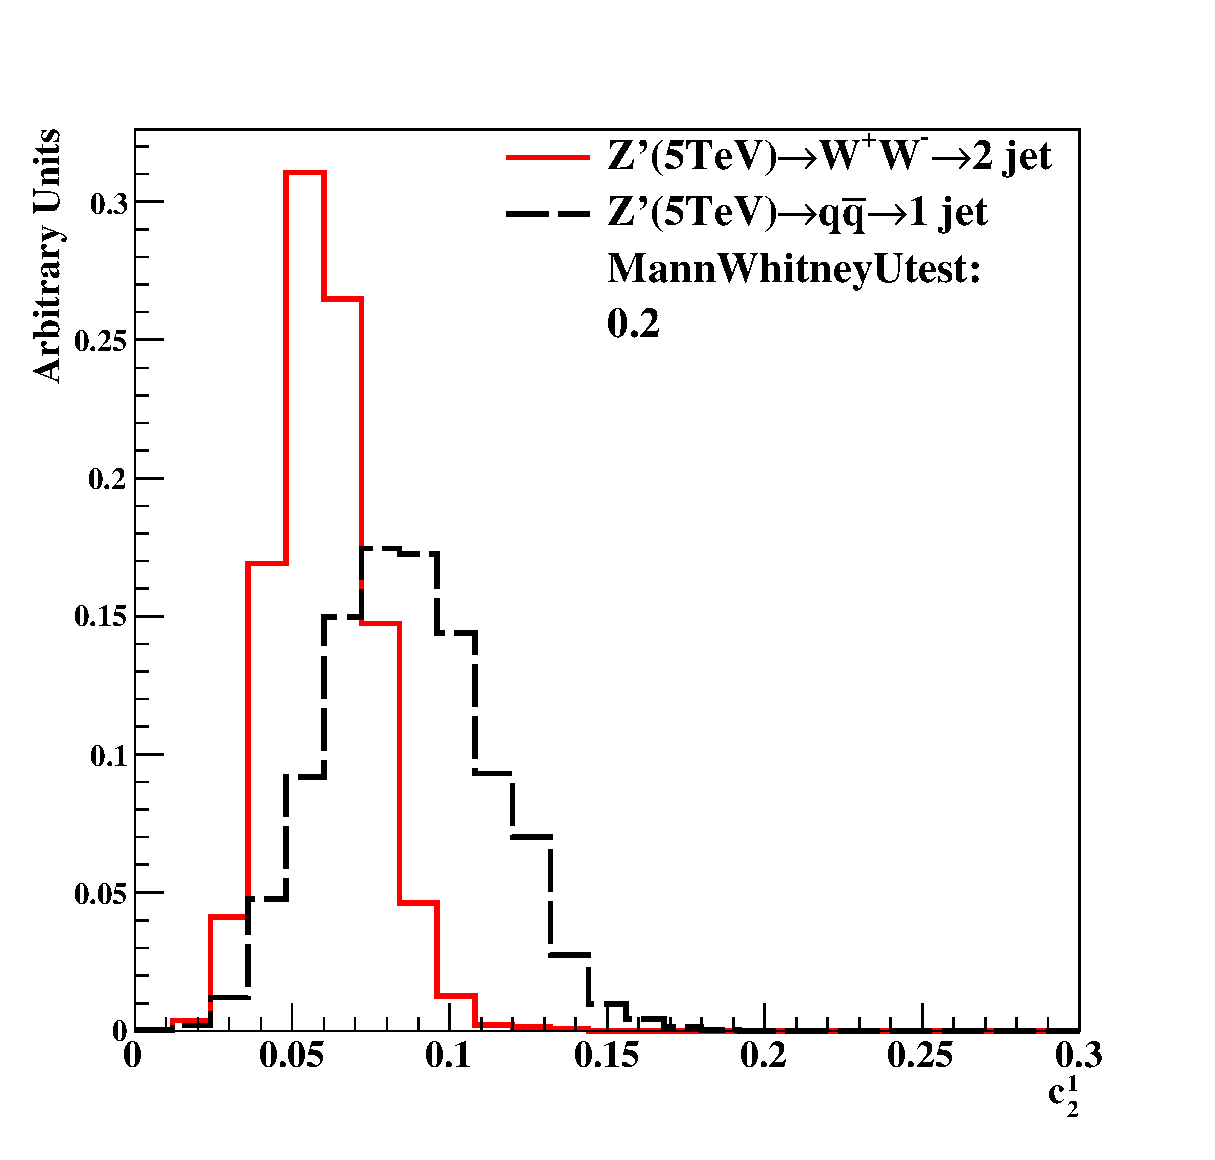
\includegraphics[width=0.22\textwidth]{figs/Dis_cluster_010_c2b1_5tev_04_Man.eps}\hfill
   }
   \subfigure[10TeV at 20$\times$20(cm$\times$cm) in cluster] {
   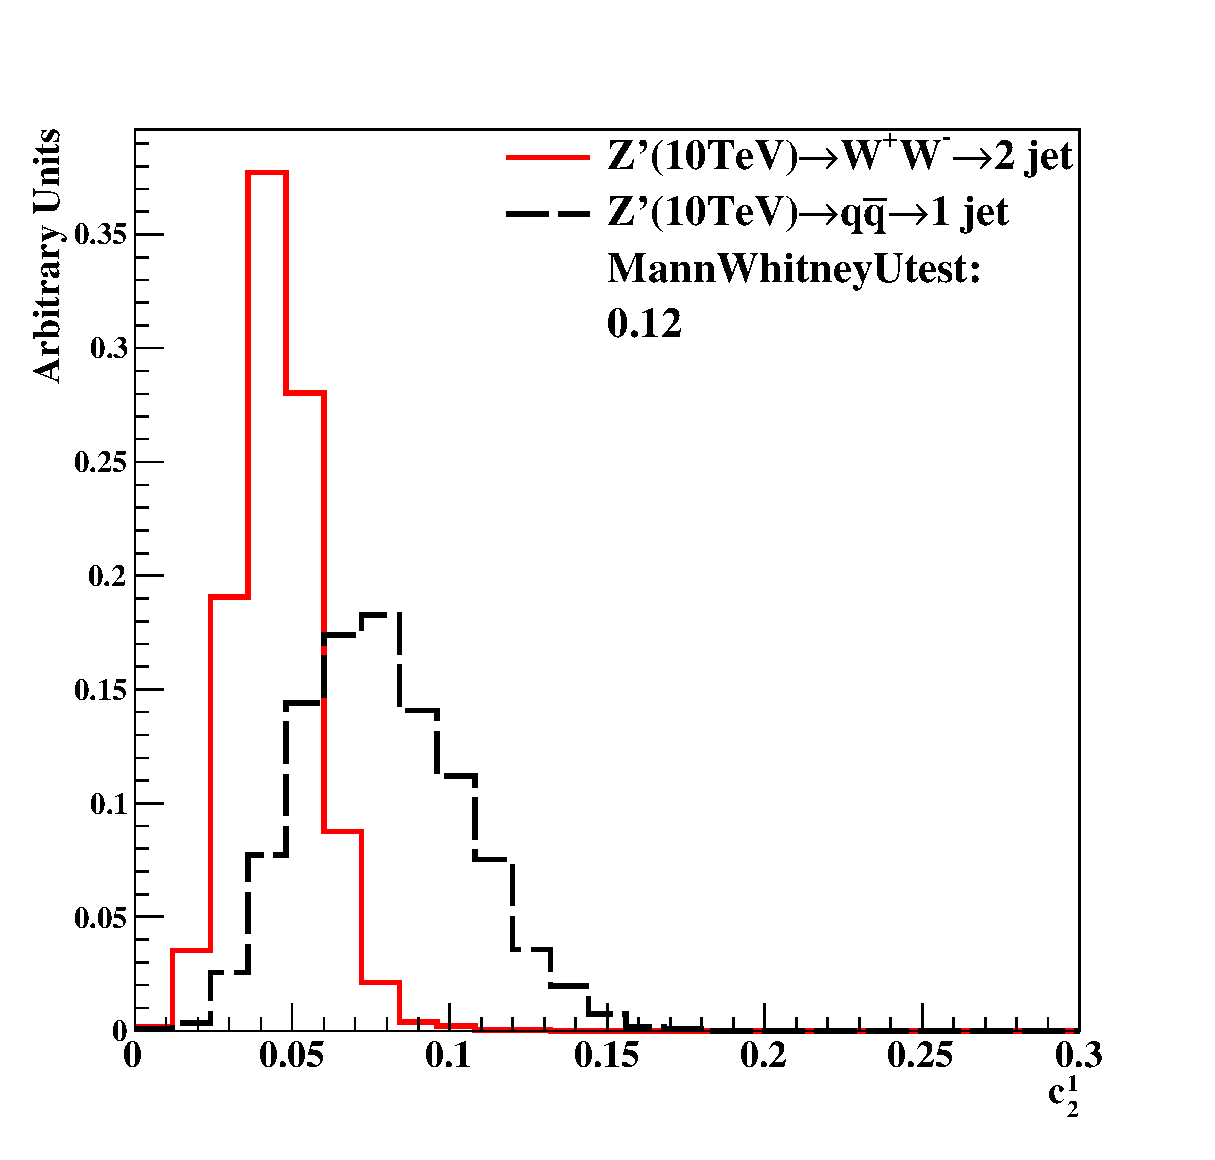
\includegraphics[width=0.22\textwidth]{figs/Dis_cluster_010_c2b1_10tev_04_Man.eps}
   }
   \subfigure[20TeV at 20$\times$20(cm$\times$cm) in cluster] {
   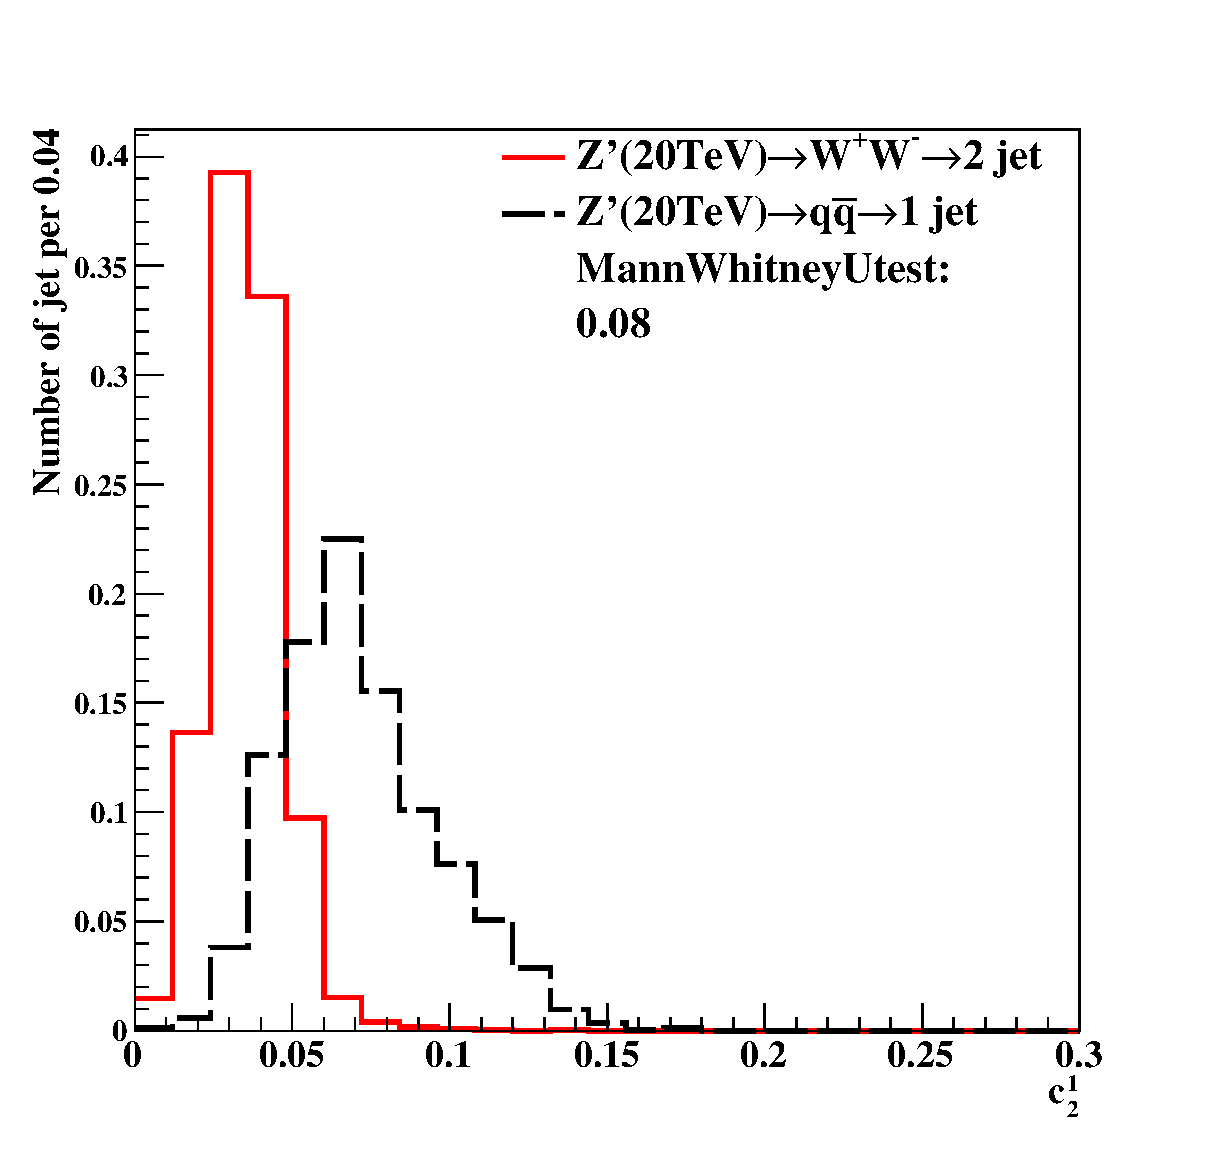
\includegraphics[width=0.22\textwidth]{figs/Dis_cluster_010_c2b1_20tev_04_Man.eps}
   }
   \subfigure[40TeV at 20$\times$20(cm$\times$cm) in cluster] {
   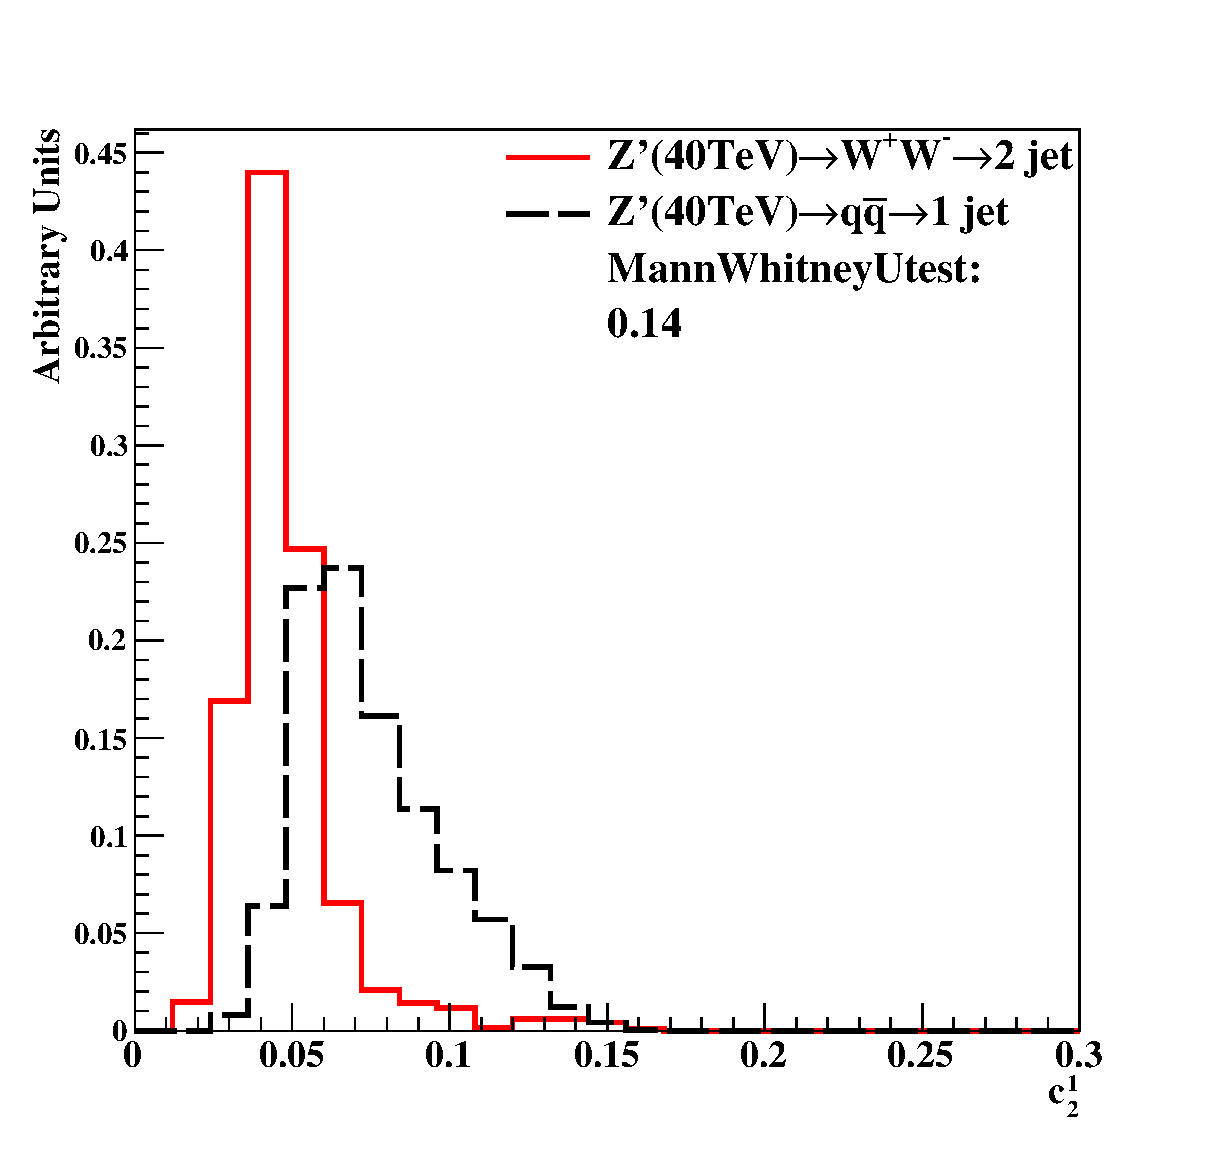
\includegraphics[width=0.22\textwidth]{figs/Dis_cluster_010_c2b1_40tev_04_Man.eps}
   }
   \subfigure[5TeV at 5$\times$5(cm$\times$cm) in cluster] {
   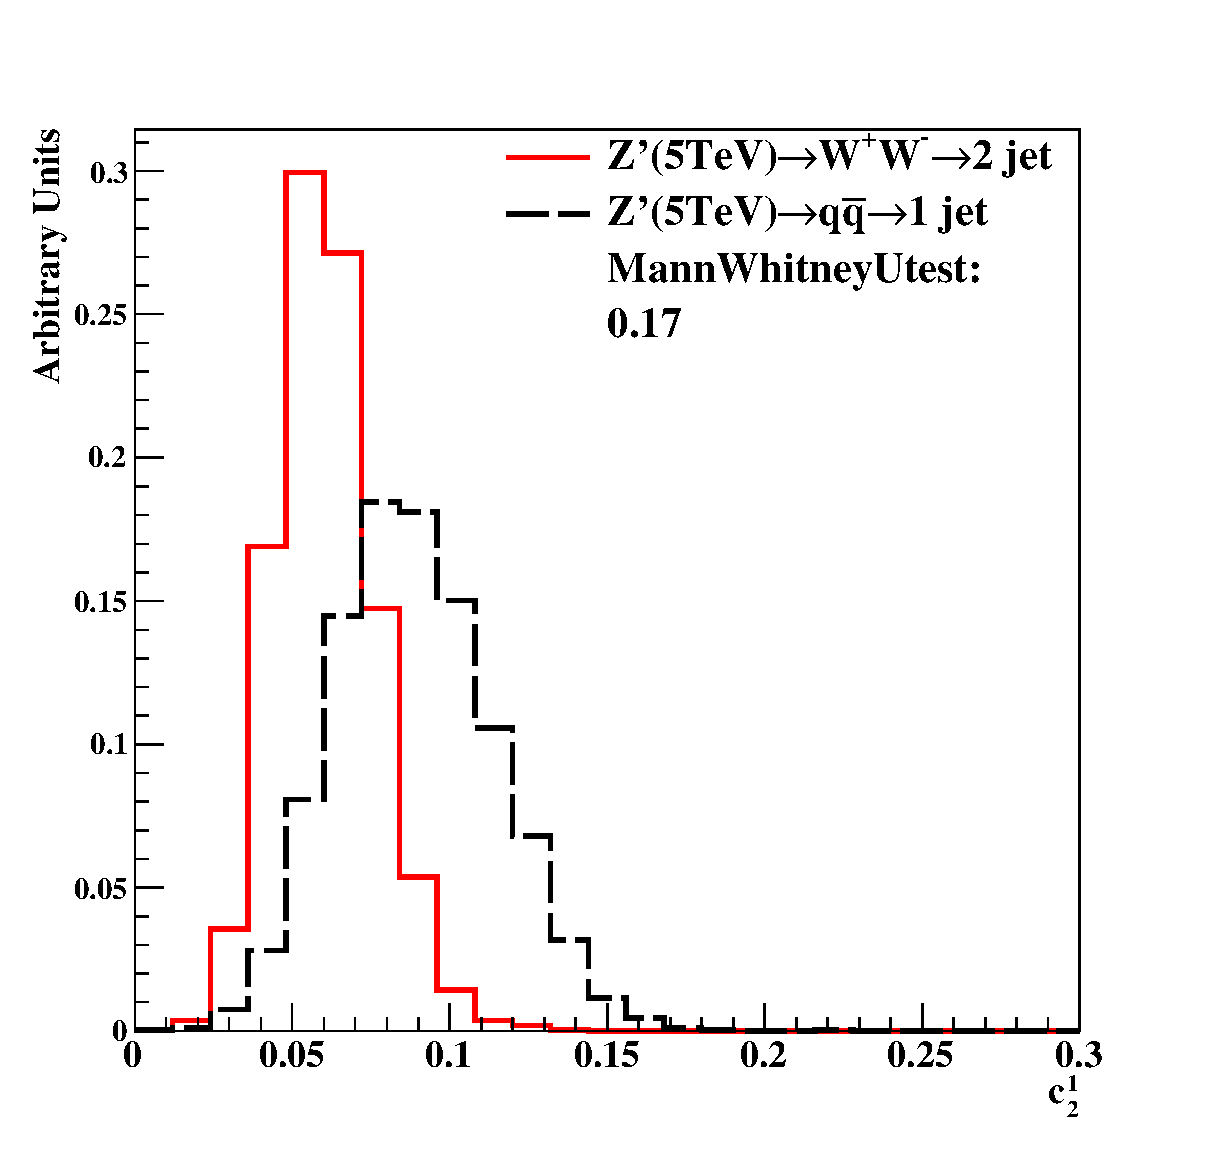
\includegraphics[width=0.22\textwidth]{figs/Dis_cluster_009_c2b1_5tev_04_Man.eps}
   }
   \subfigure[10TeV at 5$\times$5(cm$\times$cm) in cluster] {
   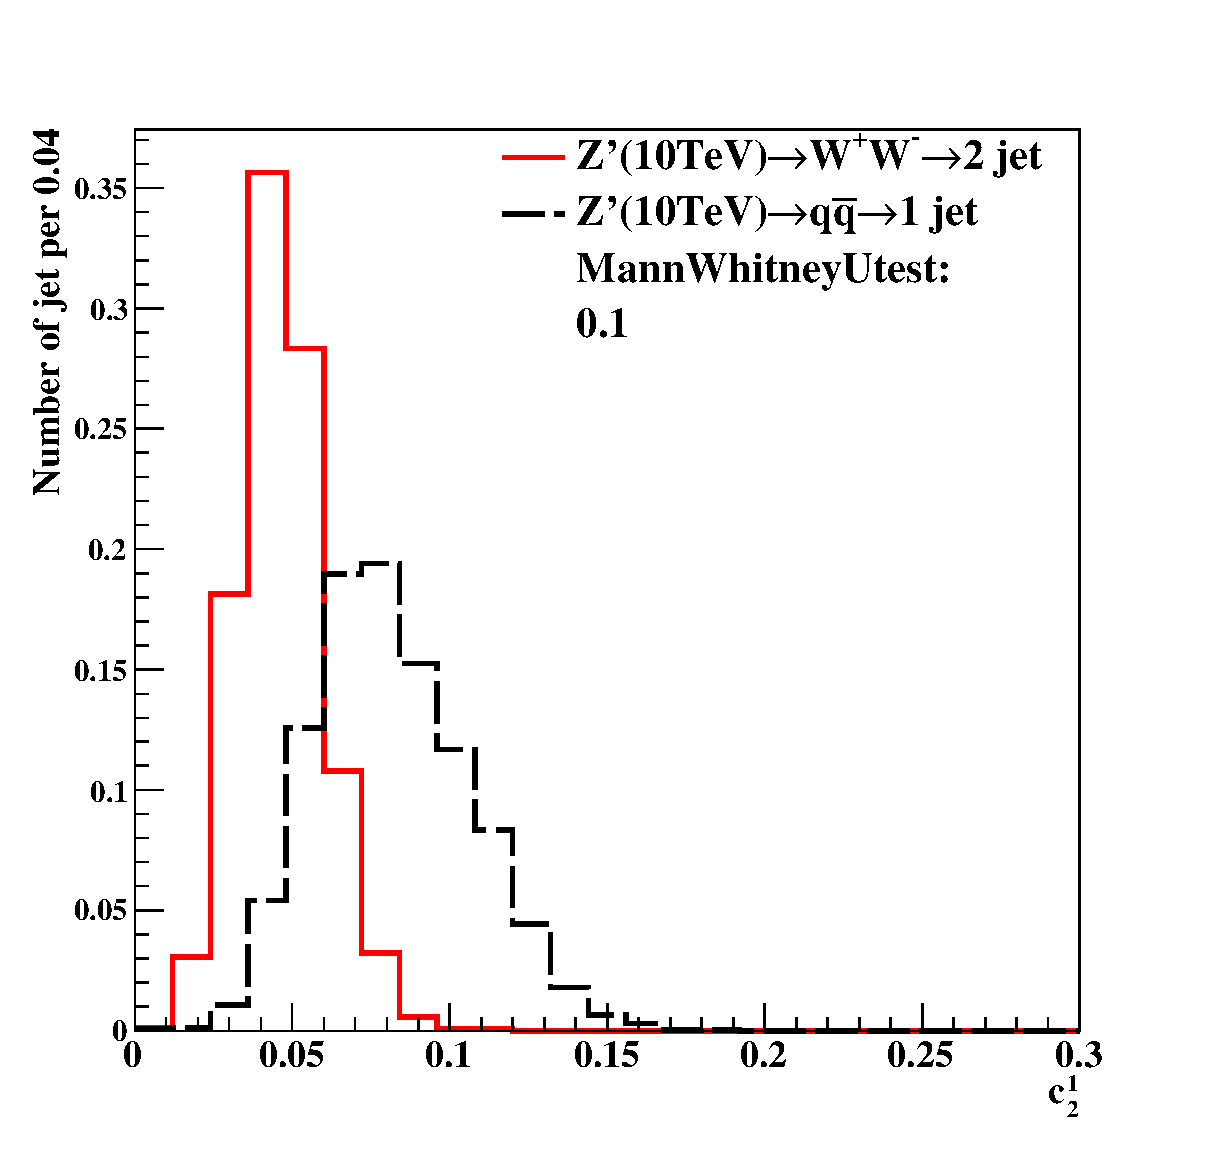
\includegraphics[width=0.22\textwidth]{figs/Dis_cluster_009_c2b1_10tev_04_Man.eps}
   }
   \subfigure[20TeV at 5$\times$5(cm$\times$cm) in cluster] {
   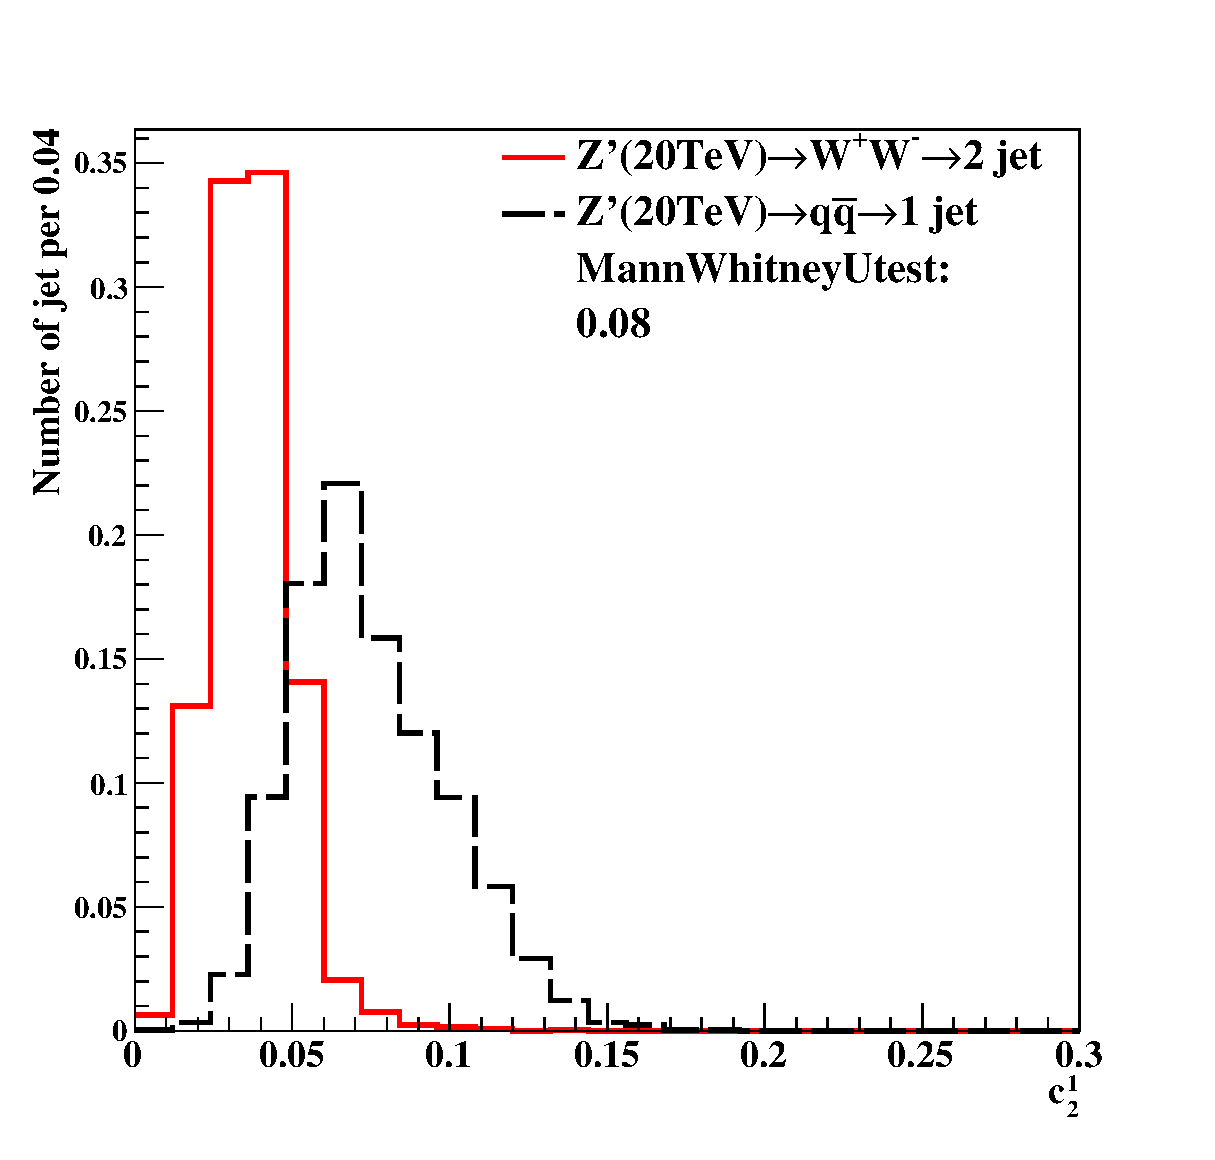
\includegraphics[width=0.22\textwidth]{figs/Dis_cluster_009_c2b1_20tev_04_Man.eps}
   }
   \subfigure[40TeV at 5$\times$5(cm$\times$cm) in cluster] {
   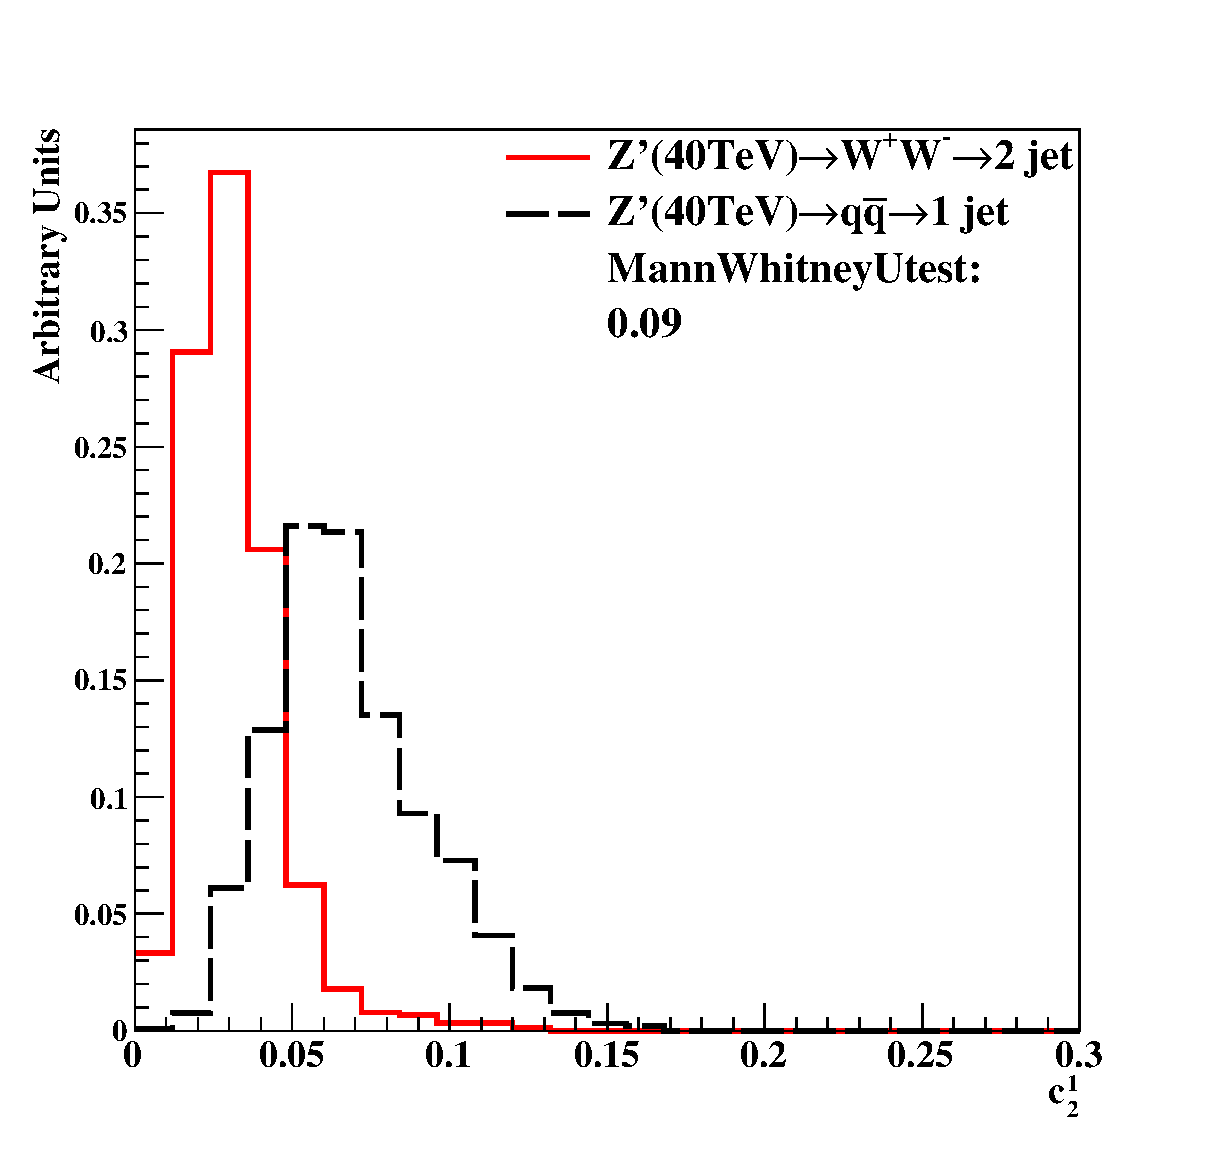
\includegraphics[width=0.22\textwidth]{figs/Dis_cluster_009_c2b1_40tev_04_Man.eps}
   }
   \subfigure[5TeV at 1$\times$1(cm$\times$cm) in cluster] {
   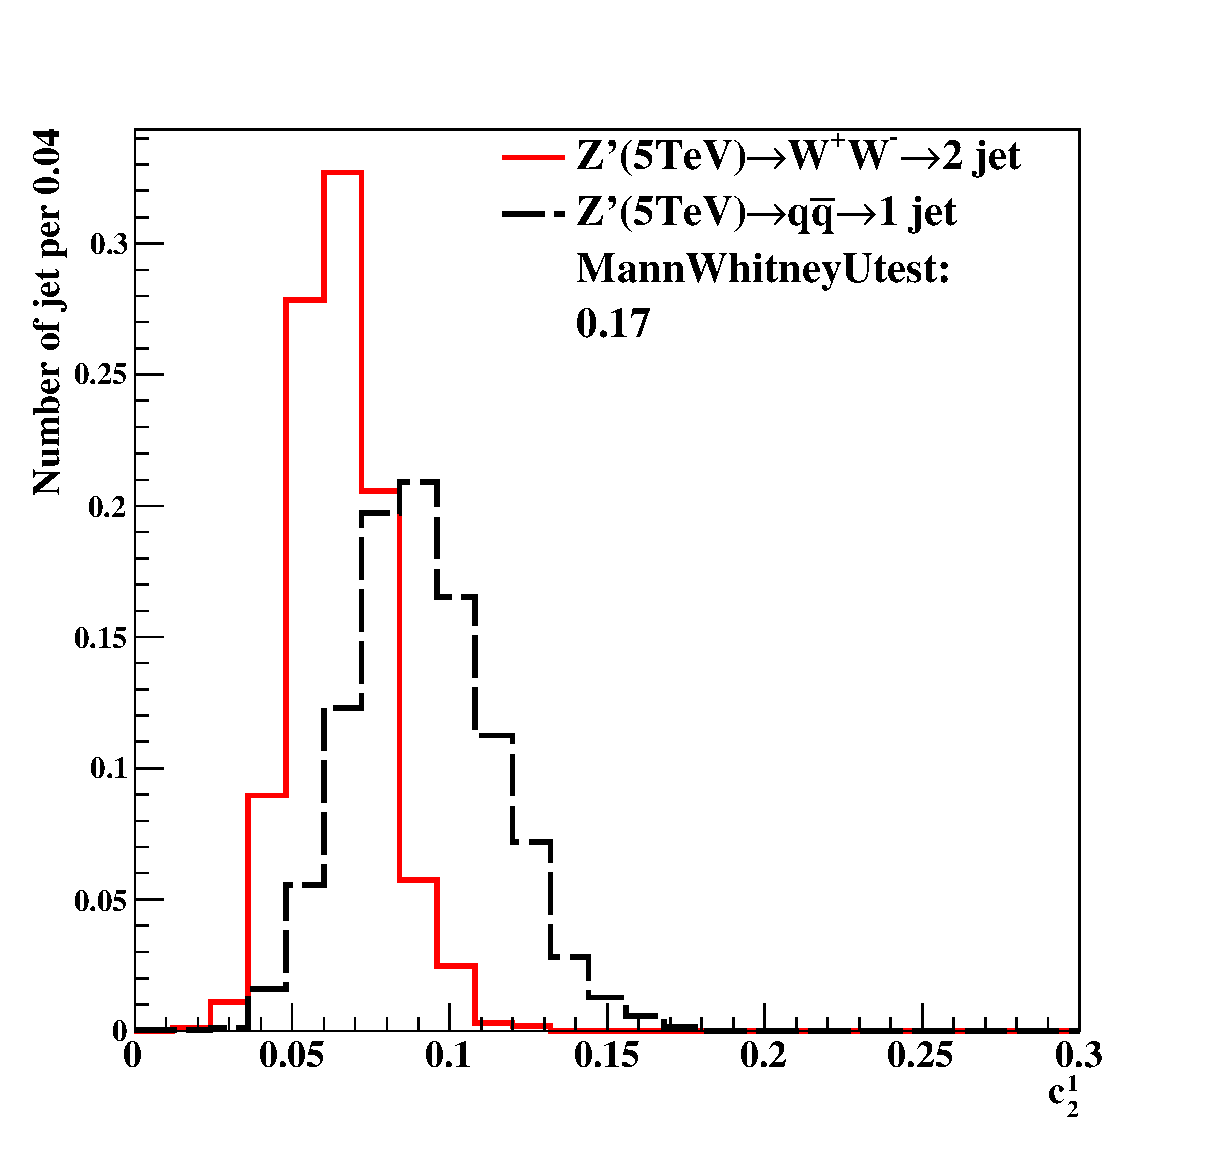
\includegraphics[width=0.22\textwidth]{figs/Dis_cluster_012_c2b1_5tev_04_Man.eps}
   }
   \subfigure[10TeV at 1$\times$1(cm$\times$cm) in cluster] {
   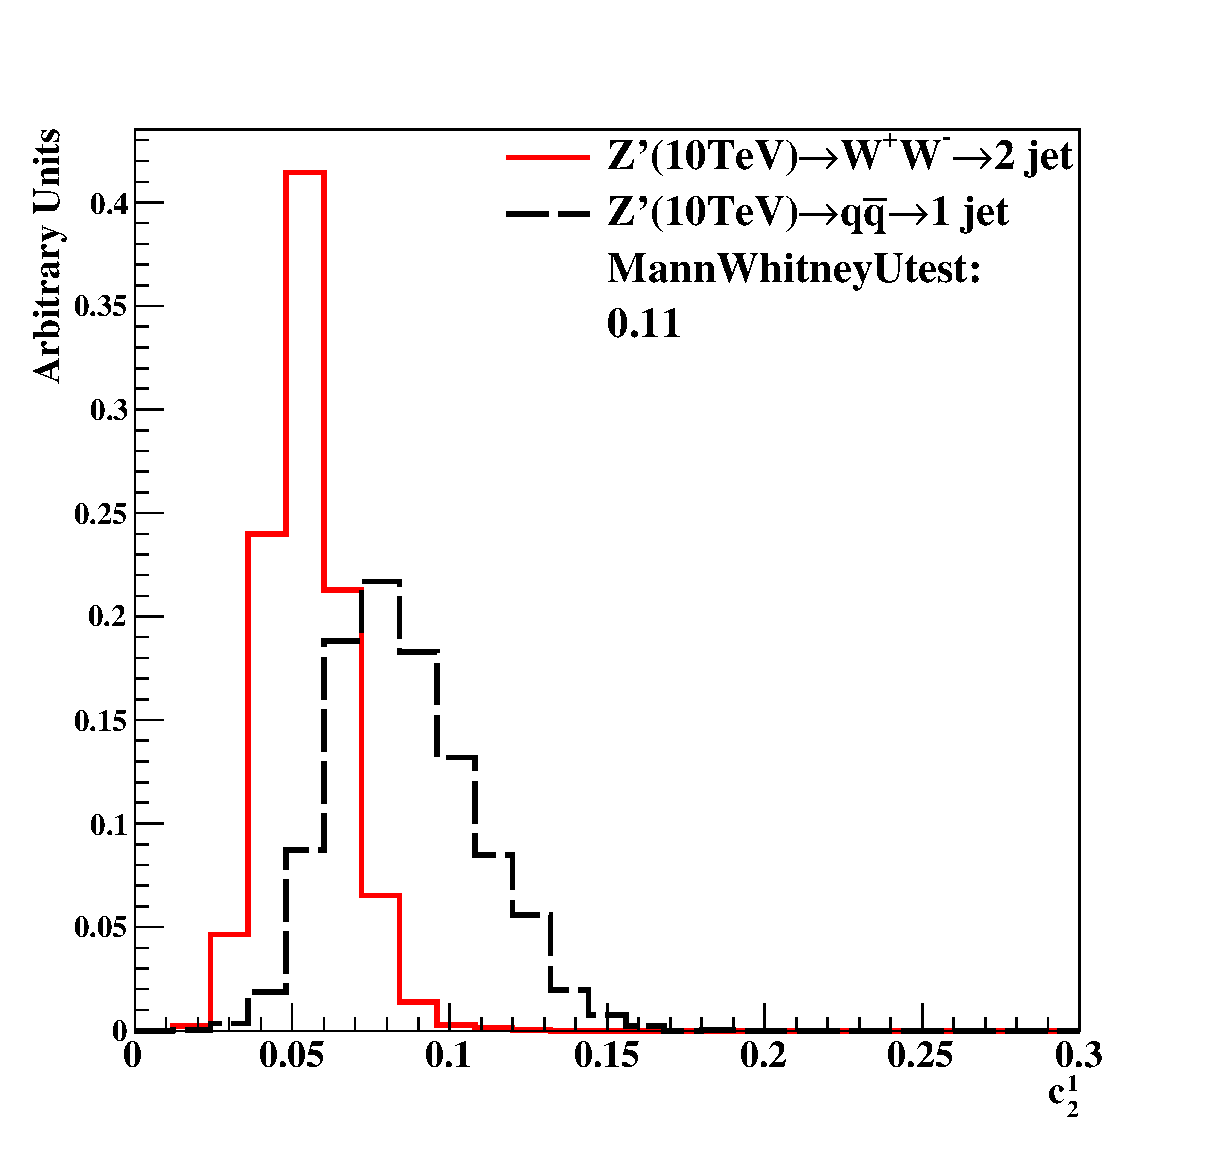
\includegraphics[width=0.22\textwidth]{figs/Dis_cluster_012_c2b1_10tev_04_Man.eps}
   }
   \subfigure[20TeV at 1$\times$1(cm$\times$cm) in cluster] {
   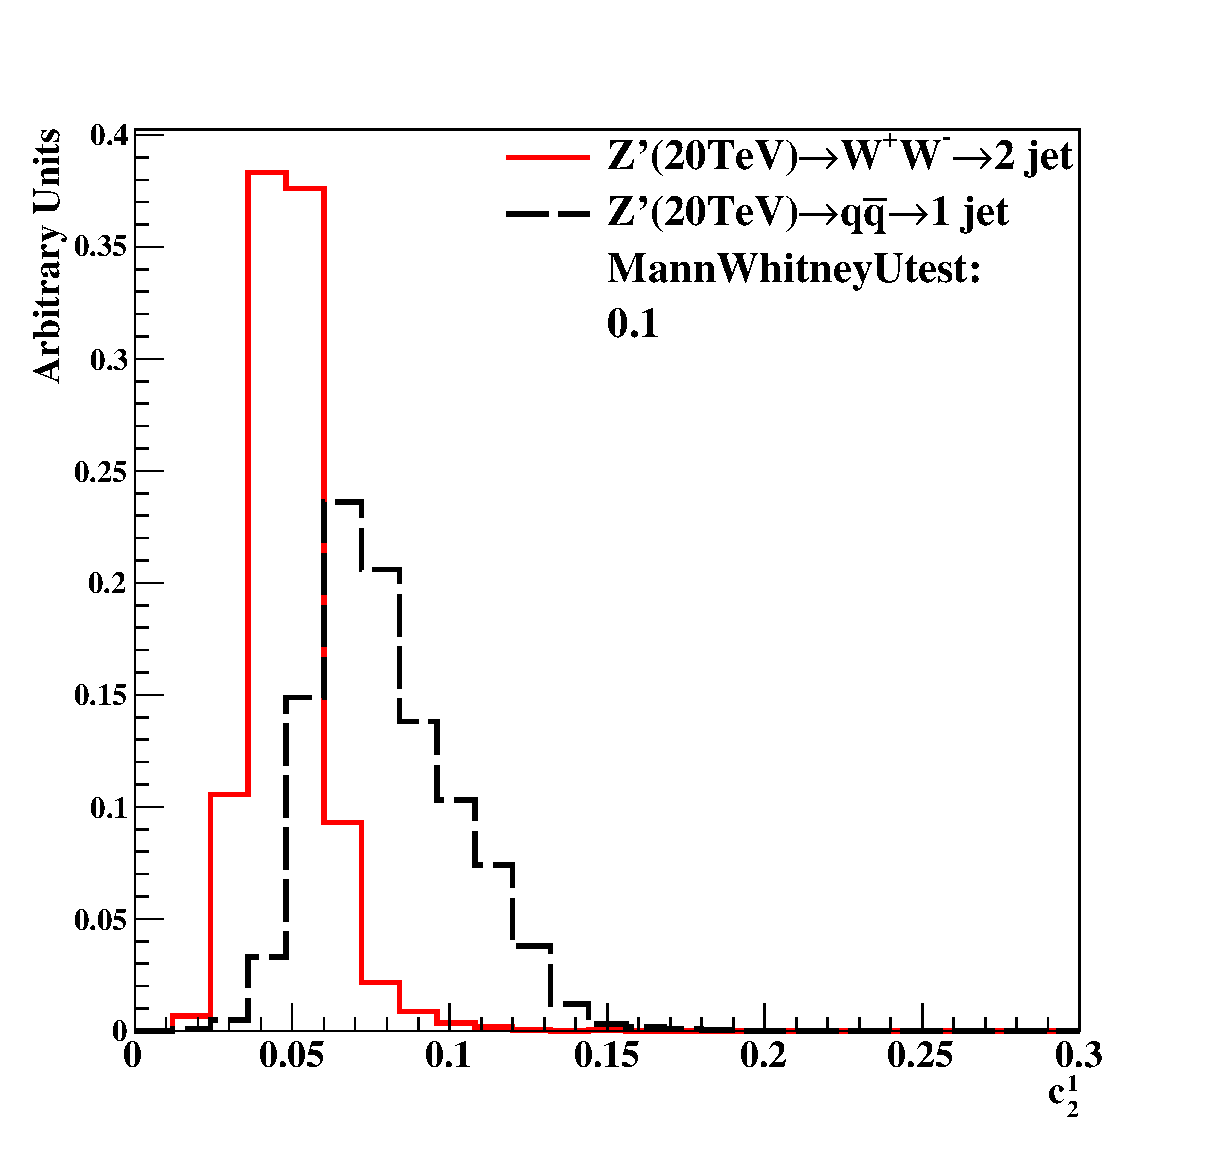
\includegraphics[width=0.22\textwidth]{figs/Dis_cluster_012_c2b1_20tev_04_Man.eps}
   }
   \subfigure[40TeV at 1$\times$1(cm$\times$cm) in cluster] {
   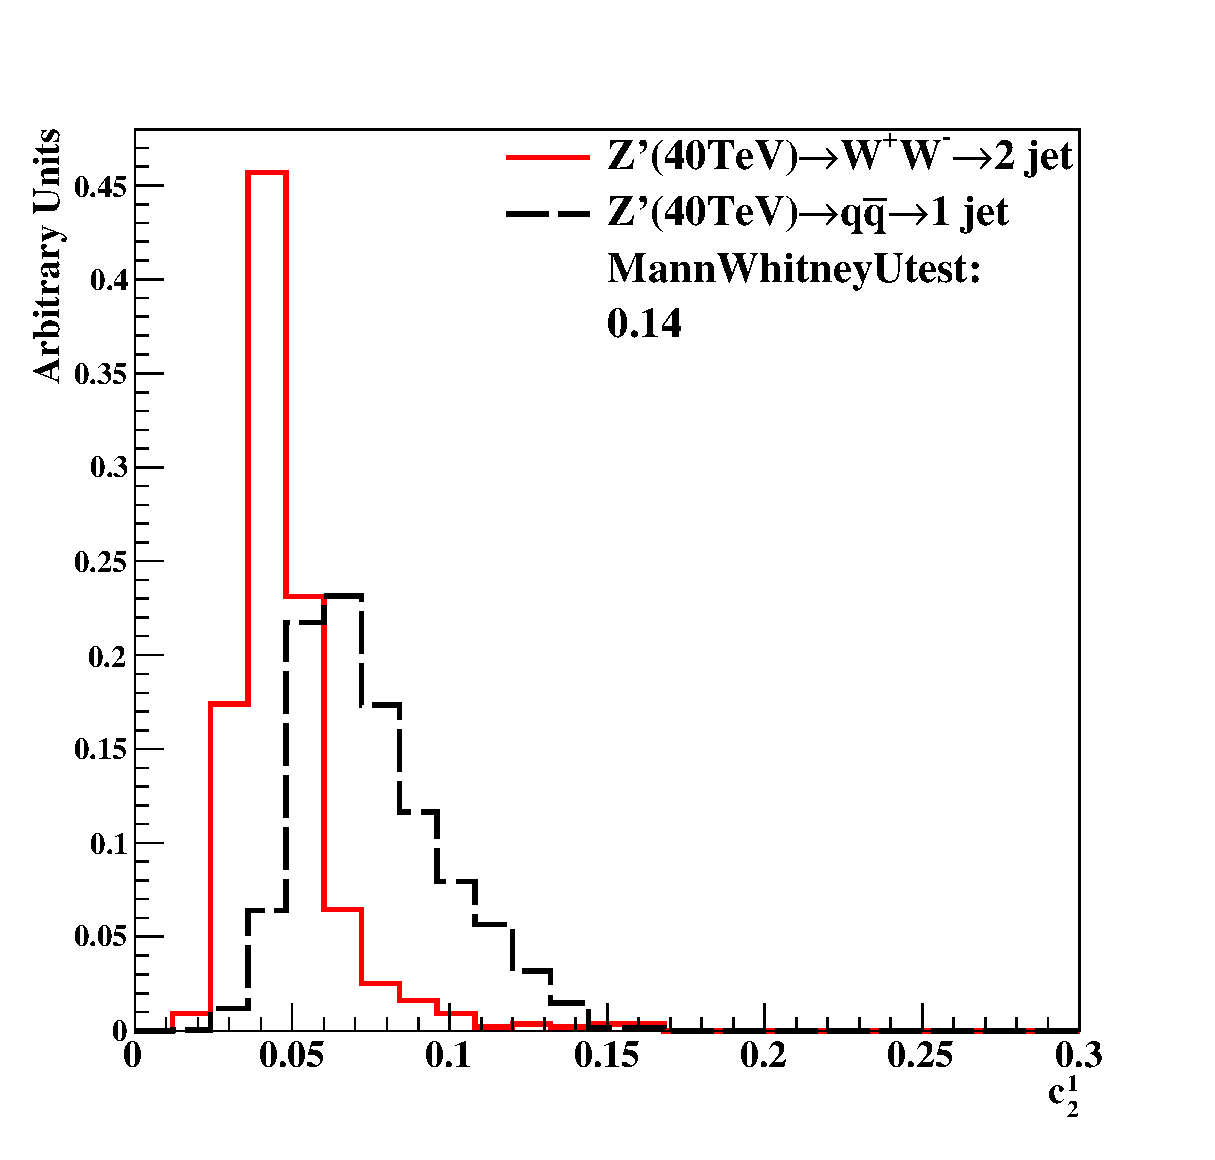
\includegraphics[width=0.22\textwidth]{figs/Dis_cluster_012_c2b1_40tev_04_Man.eps}
   }
\end{center}
\caption{Distributions of Mann-Whitney value U in 5,10,20,40TeV energy collision for $c_2^{(1)}$ in different detector sizes WithoutCut. Cell Size in 20$\times$20, 5$\times$5, and 1$\times$1(cm$\times$cm) are shown here.}
\label{fig:cluster_tau21_tau32}
\end{figure}

\begin{figure}
\begin{center}
   \subfigure[5 TeV using cluster method with New2 after cut Method] {
   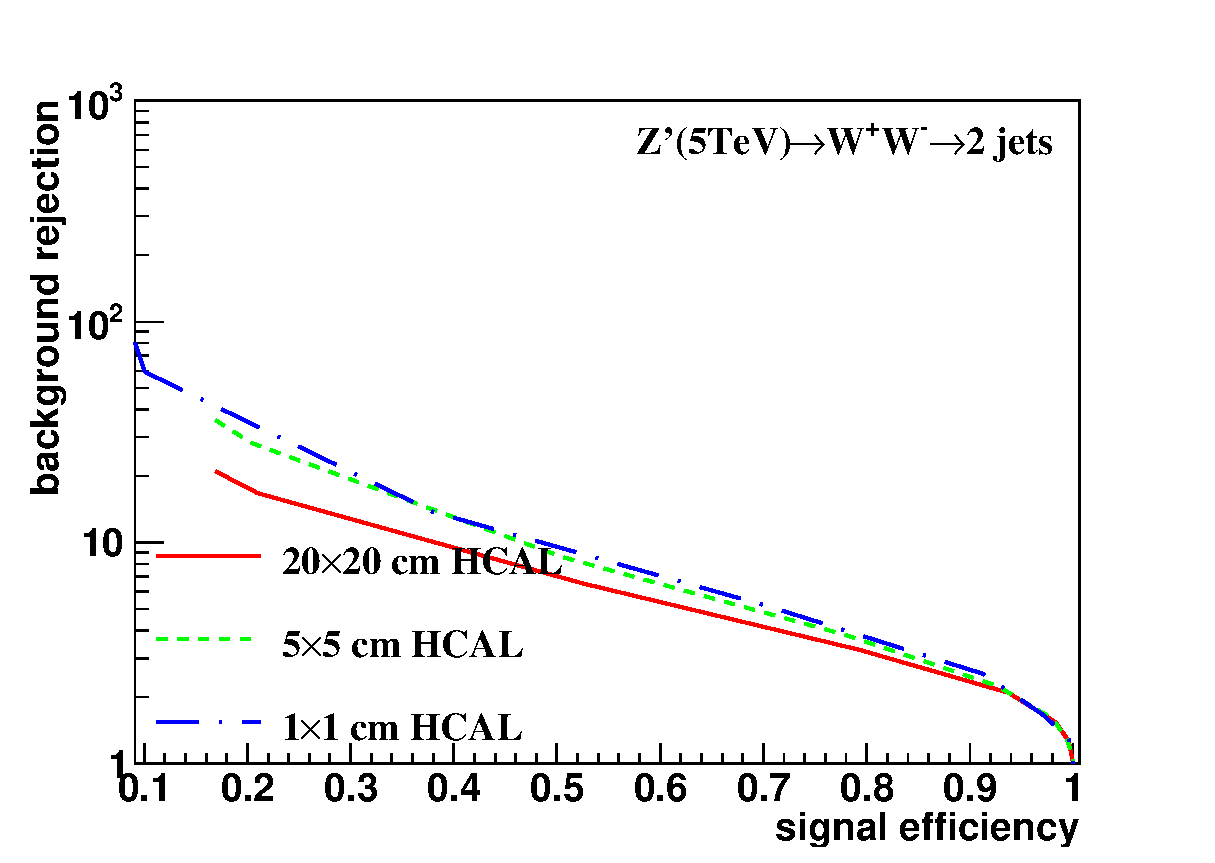
\includegraphics[width=0.43\textwidth]{figs/cluster_c2b1_5tev_eff_1_New2_no_cut_25bins.eps}\hfill
   }
   \subfigure[10 TeV using cluster method with New2 after cut Method] {
   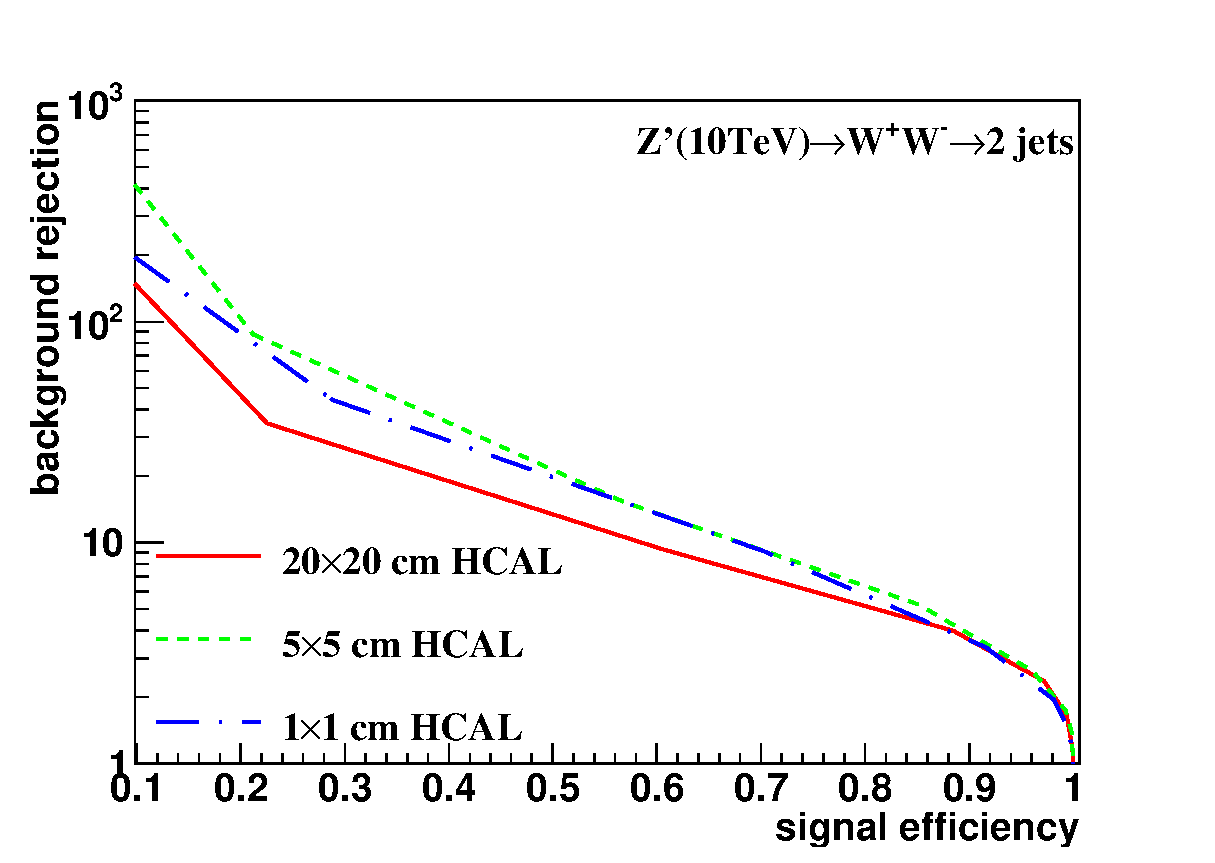
\includegraphics[width=0.43\textwidth]{figs/cluster_c2b1_10tev_eff_1_New2_no_cut_25bins.eps}
   }
   \subfigure[20 TeV using cluster method with New2 after cut Method] {
   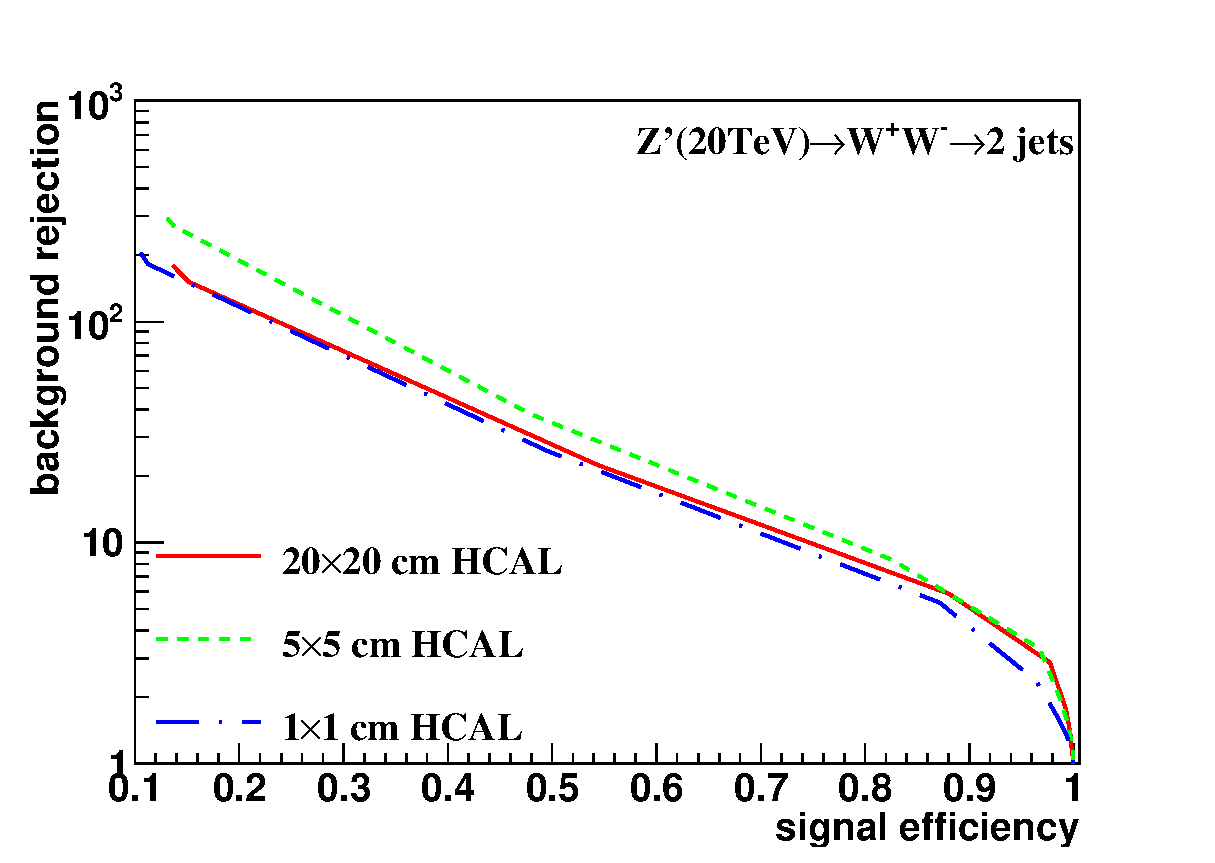
\includegraphics[width=0.43\textwidth]{figs/cluster_c2b1_20tev_eff_1_New2_no_cut_25bins.eps}
   }
   \subfigure[40 TeV using cluster method with New2 after cut Method] {
   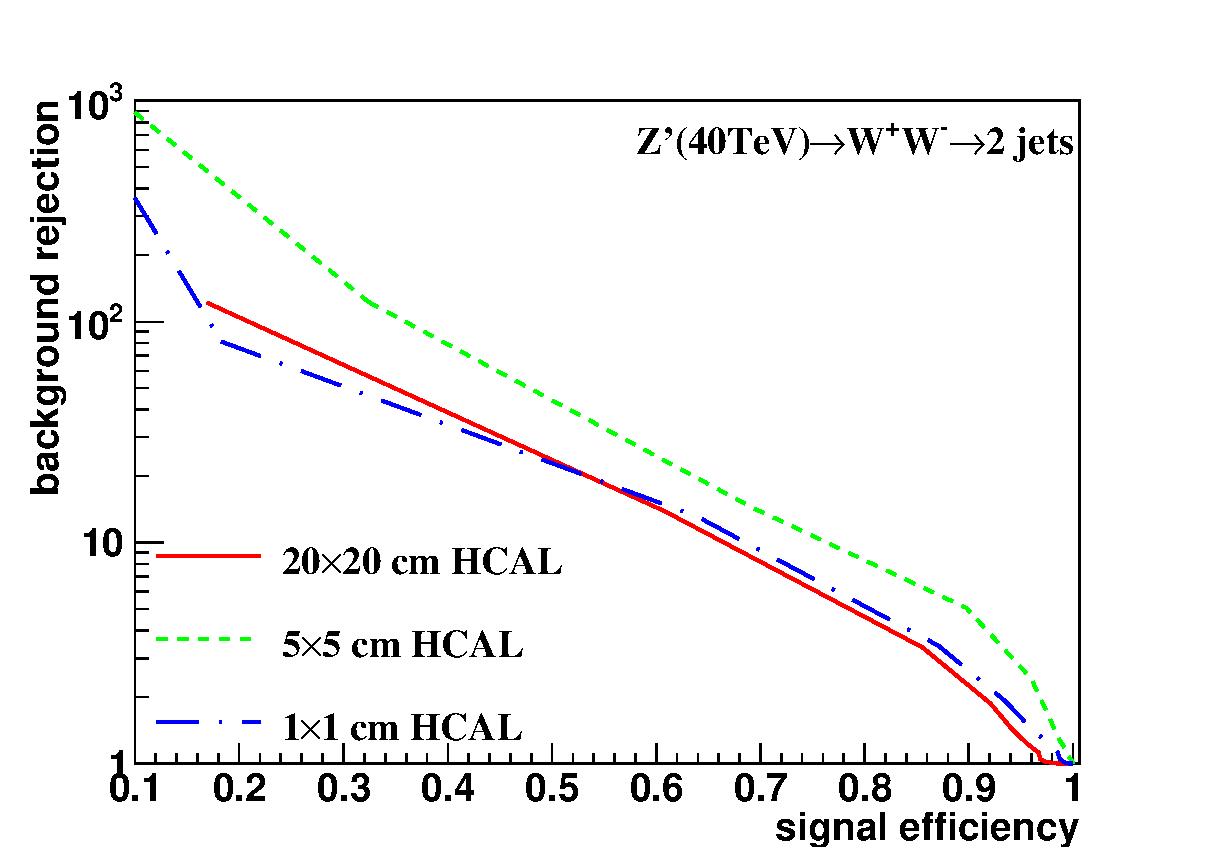
\includegraphics[width=0.43\textwidth]{figs/cluster_c2b1_40tev_eff_1_New2_no_cut_25bins.eps}
   }
\end{center}
\caption{Signal efficiency versus background rejection rate using c2b1.The energies of collision at (a)5, (b)10, (c)20, (d)40TeV are shown here. In each picture, the three ROC curves correspond to different detector sizes.}
\label{fig:cluster_c2b1}
\end{figure}
\fi

%25bins
\begin{figure}
\begin{center}
   \subfigure[5TeV at 20$\times$20(cm$\times$cm) in 0.5GeV] {
   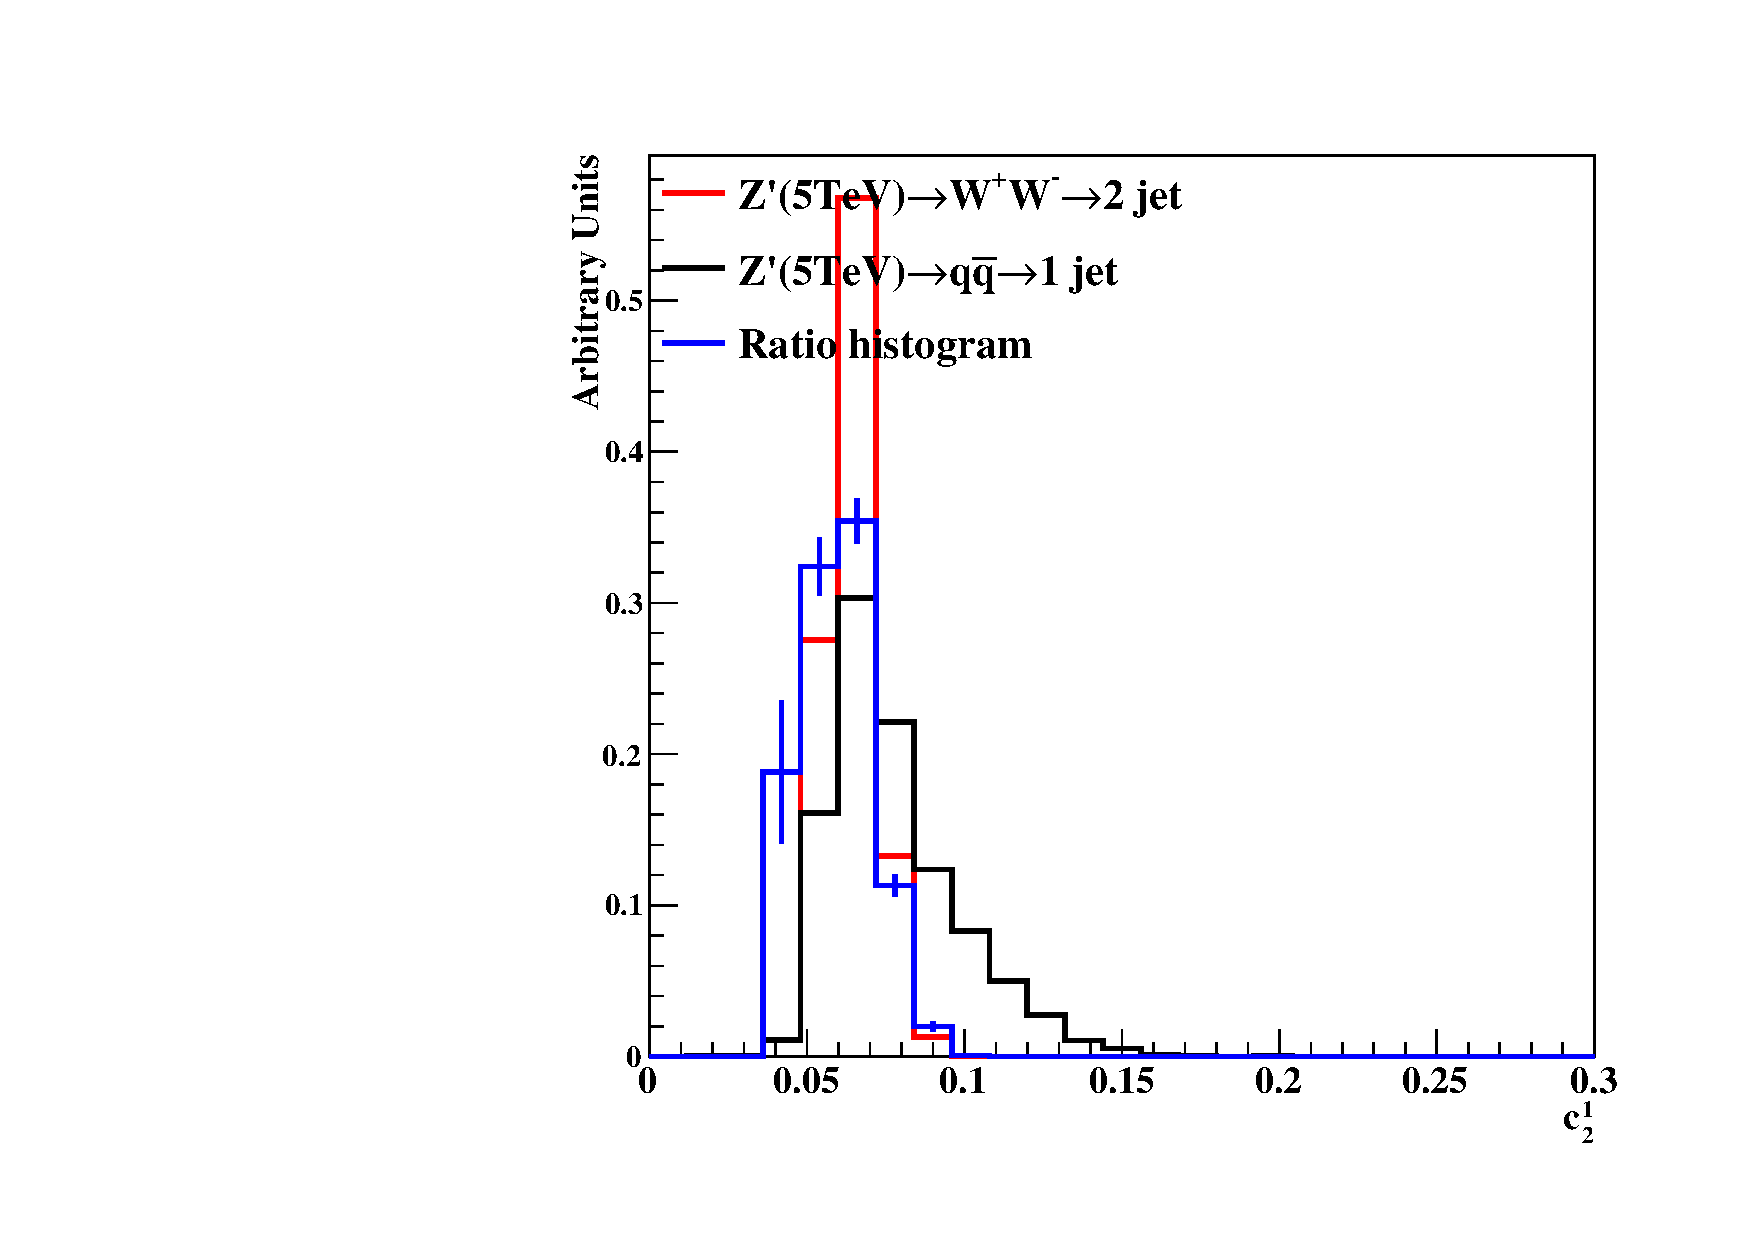
\includegraphics[width=0.22\textwidth]{figs/Rawhit_05GeV_010_c2b1_5tev_04_no_cut_25bins_Ratio.pdf}\hfill
   }
   \subfigure[10TeV at 20$\times$20(cm$\times$cm) in 0.5GeV] {
   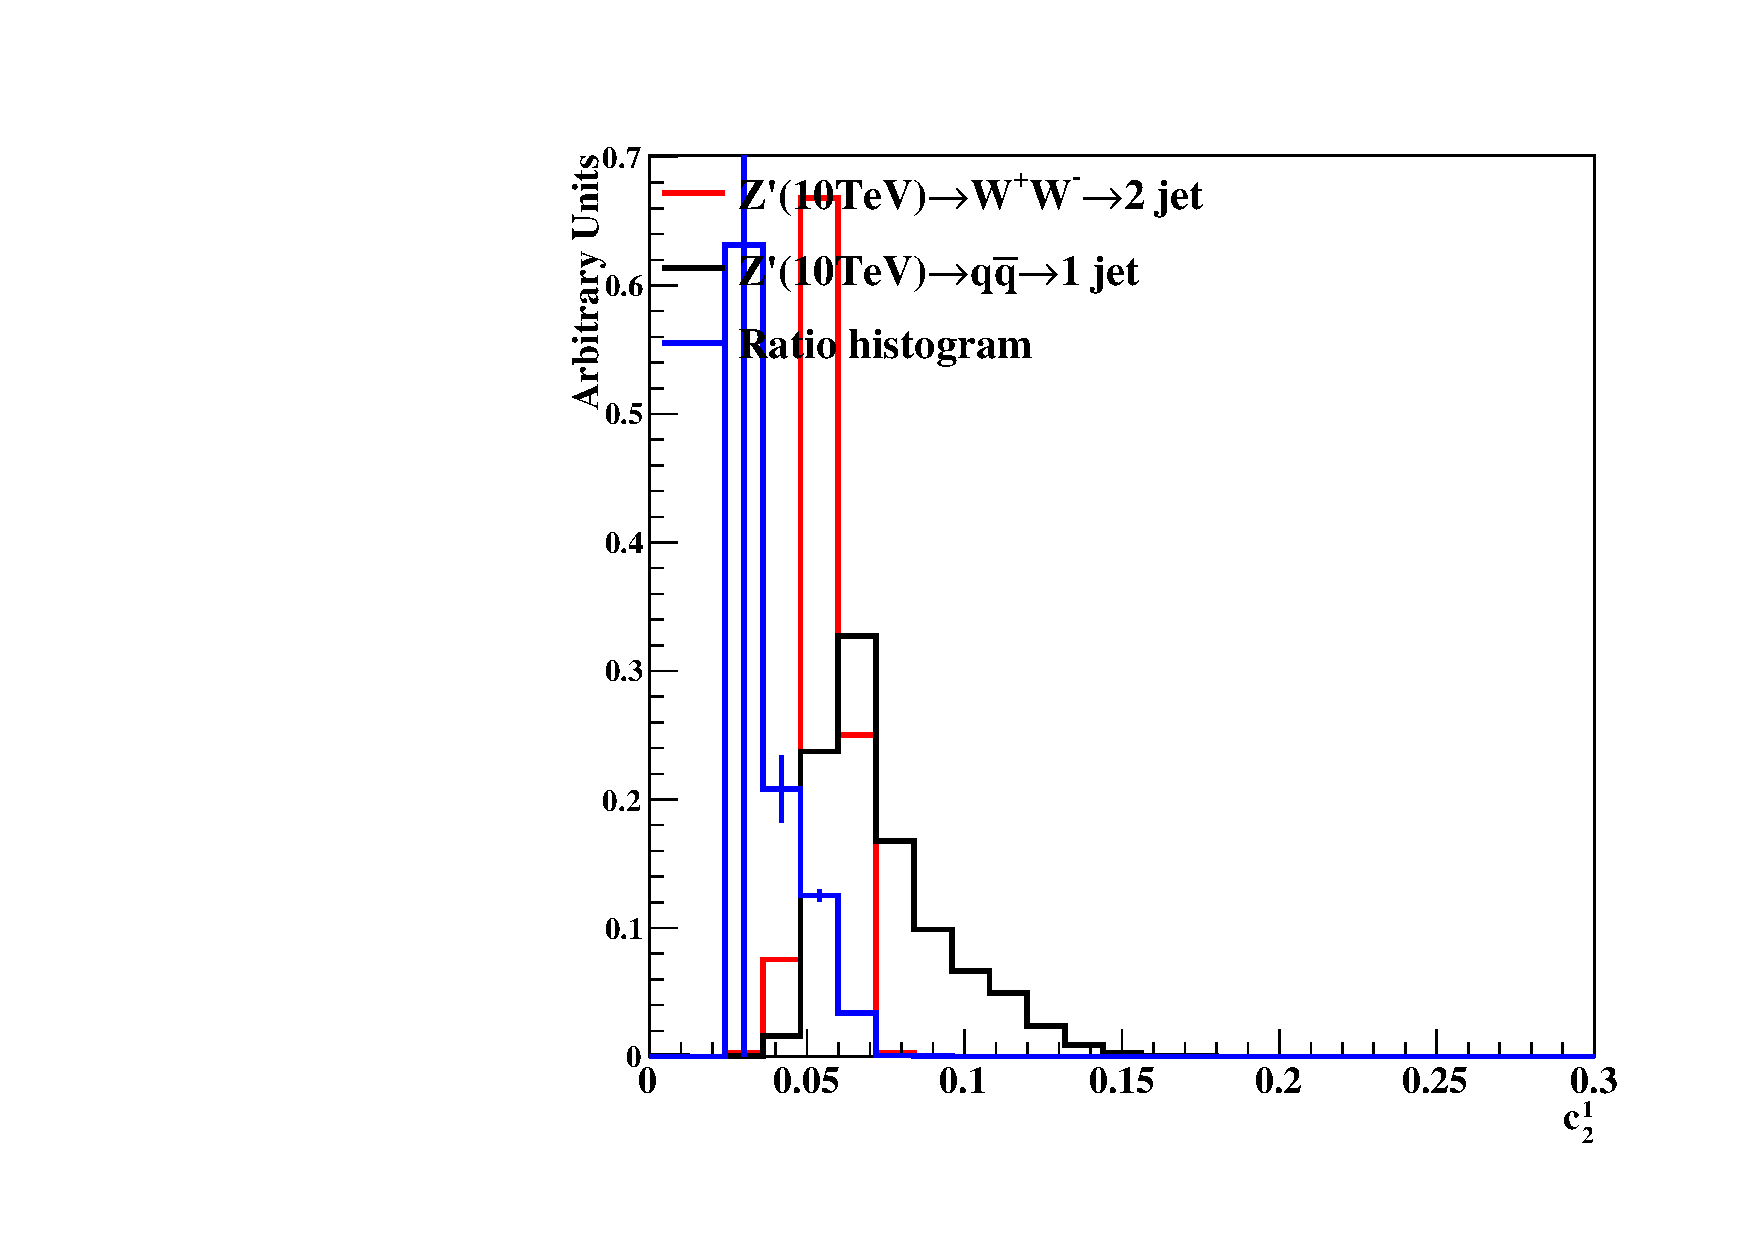
\includegraphics[width=0.22\textwidth]{figs/Rawhit_05GeV_010_c2b1_10tev_04_no_cut_25bins_Ratio.pdf}
   }
   \subfigure[20TeV at 20$\times$20(cm$\times$cm) in 0.5GeV] {
   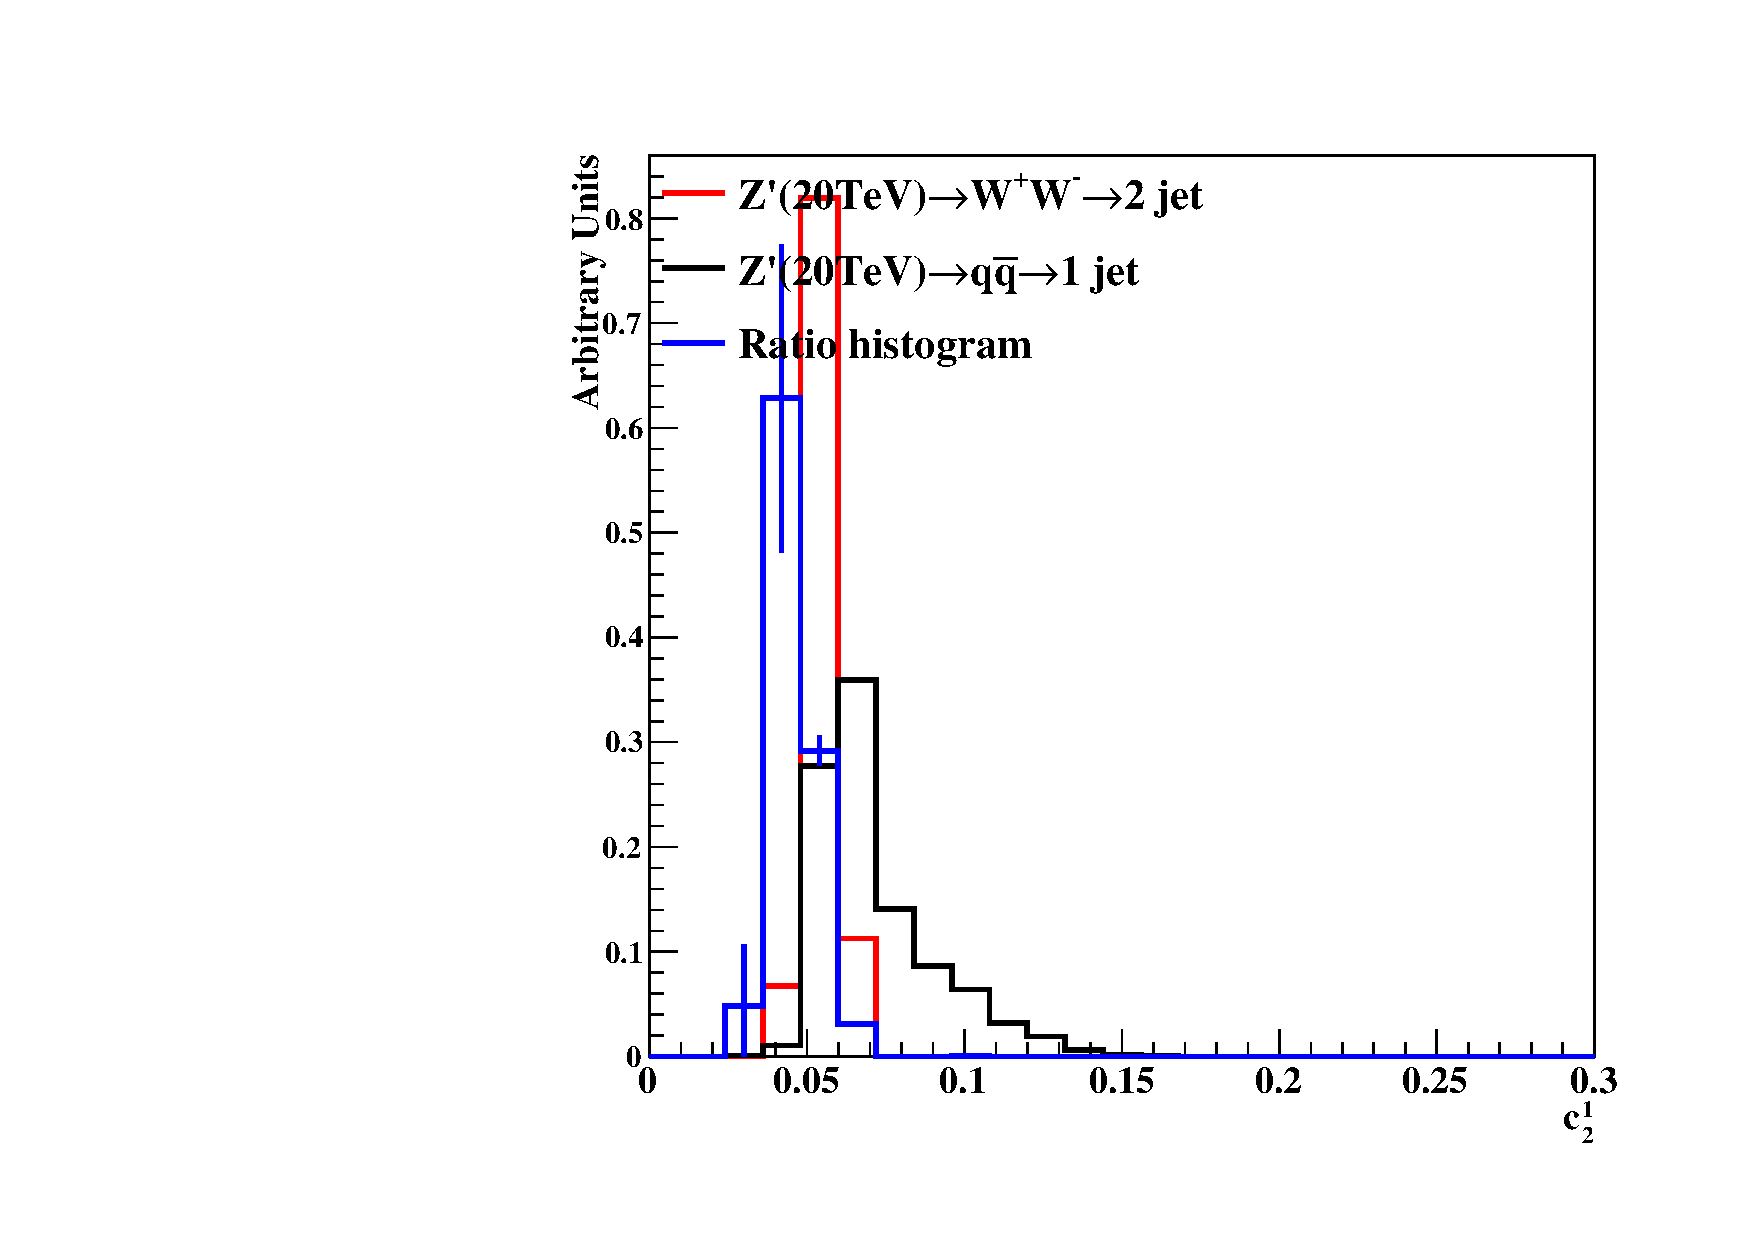
\includegraphics[width=0.22\textwidth]{figs/Rawhit_05GeV_010_c2b1_20tev_04_no_cut_25bins_Ratio.pdf}
   }
   \subfigure[40TeV at 20$\times$20(cm$\times$cm) in 0.5GeV] {
   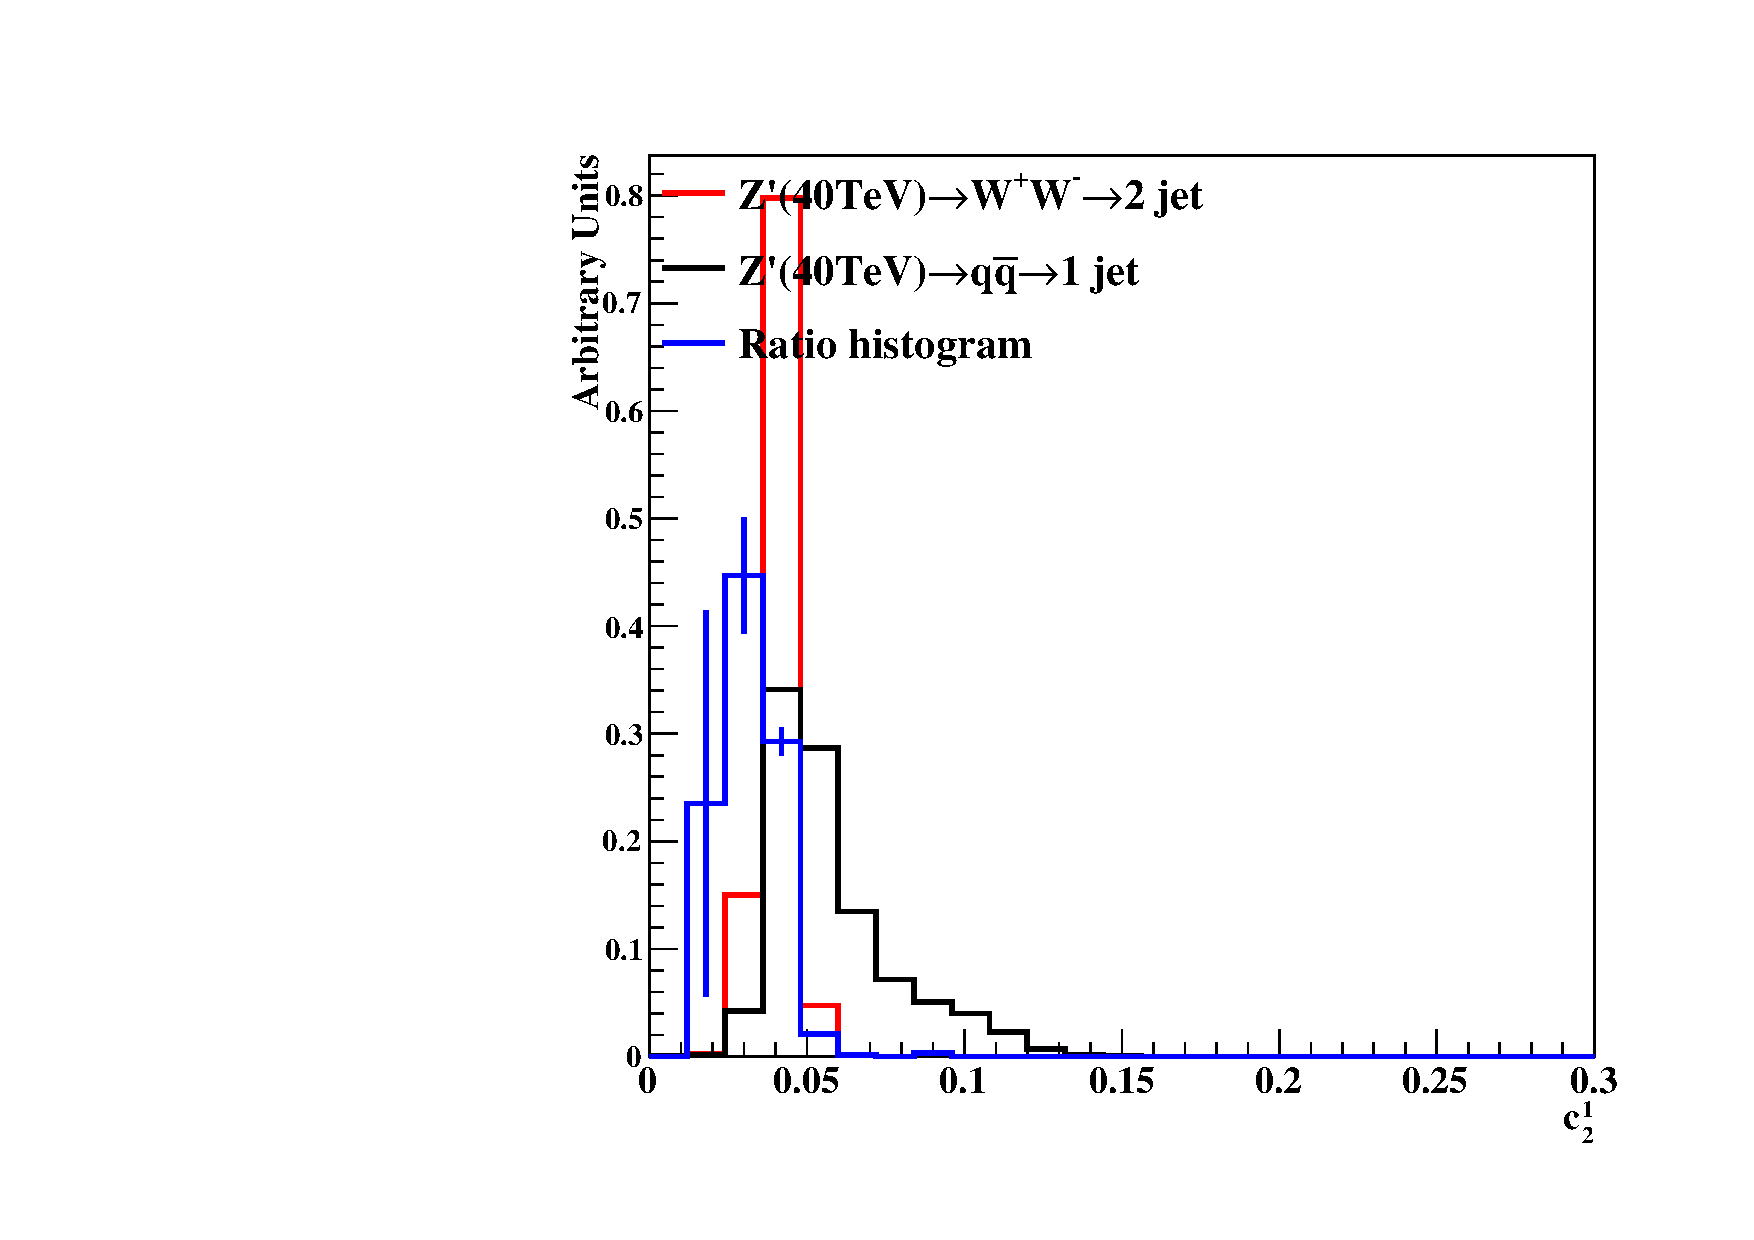
\includegraphics[width=0.22\textwidth]{figs/Rawhit_05GeV_010_c2b1_40tev_04_no_cut_25bins_Ratio.pdf}
   }
   \subfigure[5TeV at 5$\times$5(cm$\times$cm) in 0.5GeV] {
   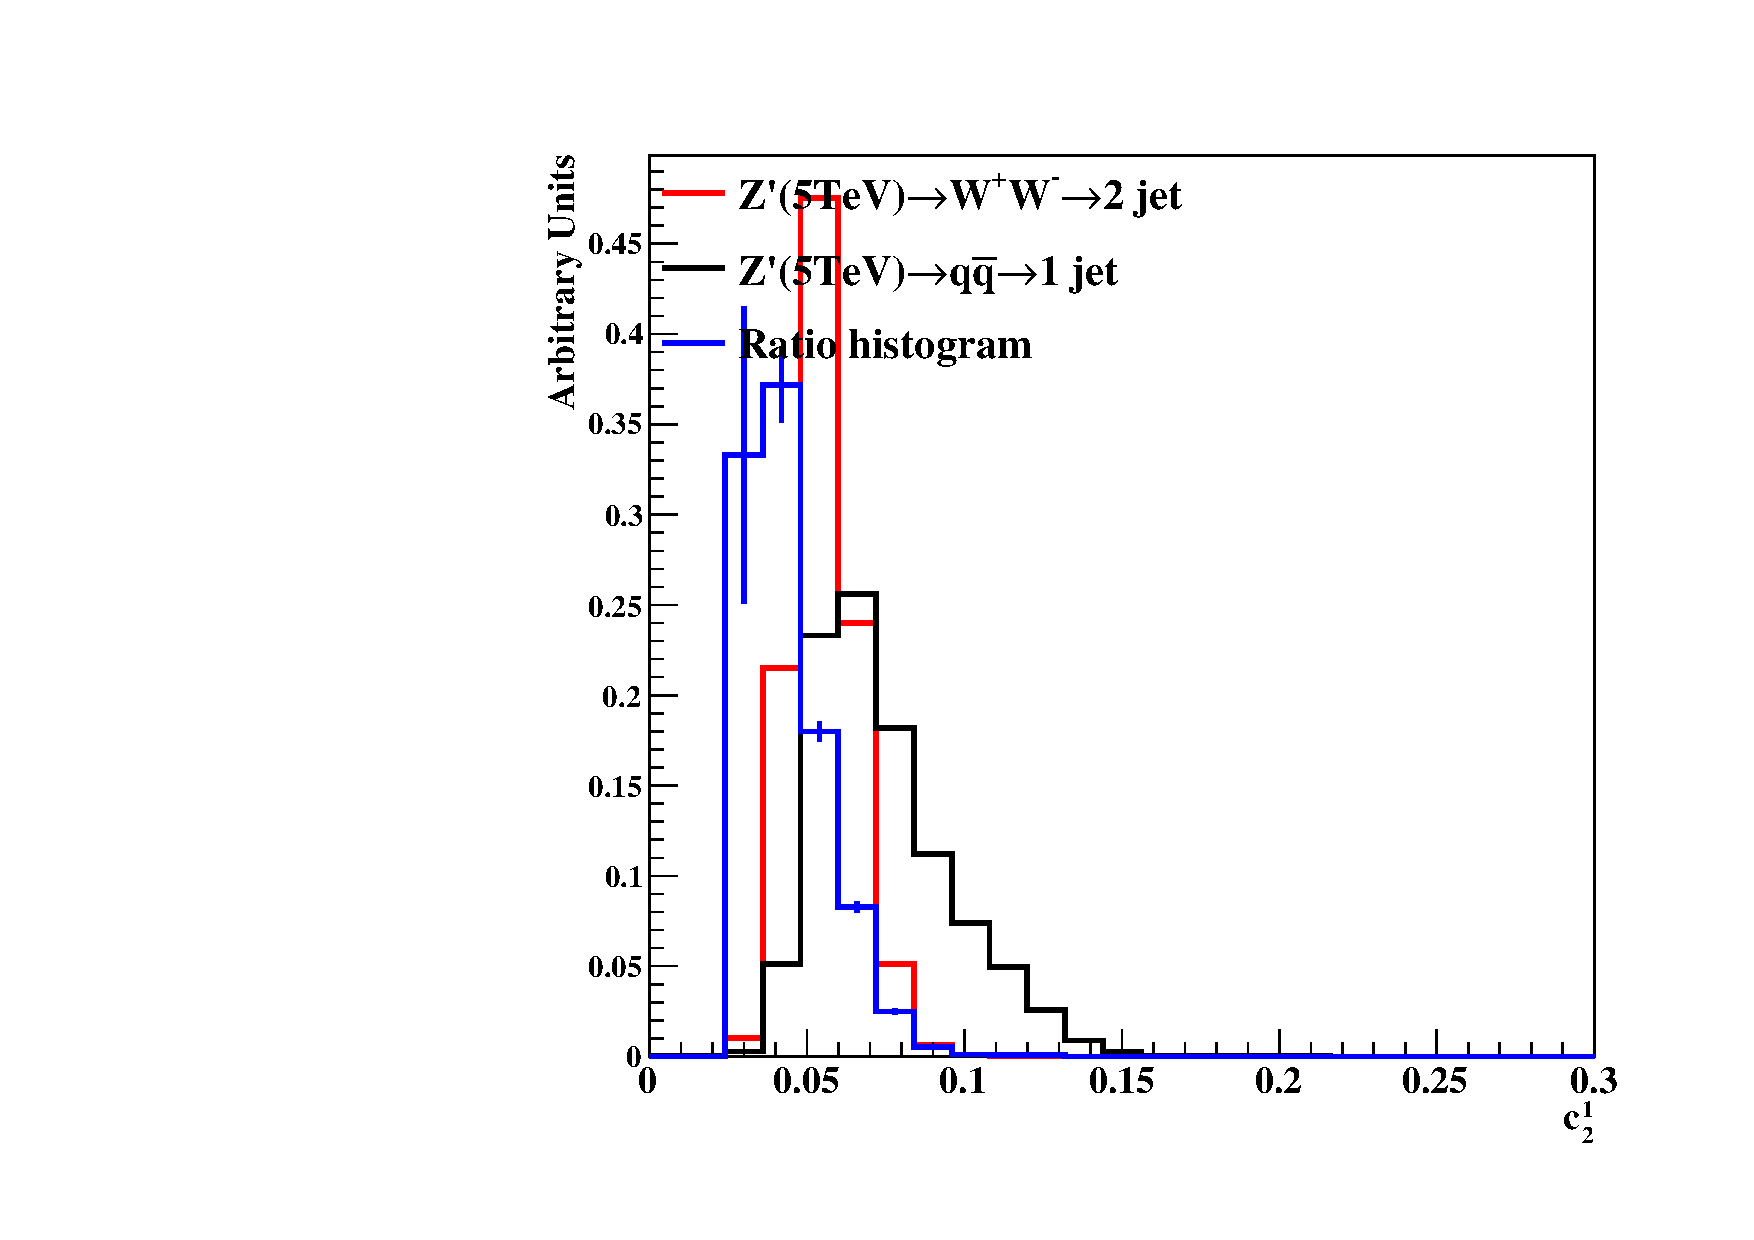
\includegraphics[width=0.22\textwidth]{figs/Rawhit_05GeV_009_c2b1_5tev_04_no_cut_25bins_Ratio.pdf}
   }
   \subfigure[10TeV at 5$\times$5(cm$\times$cm) in 0.5GeV] {
   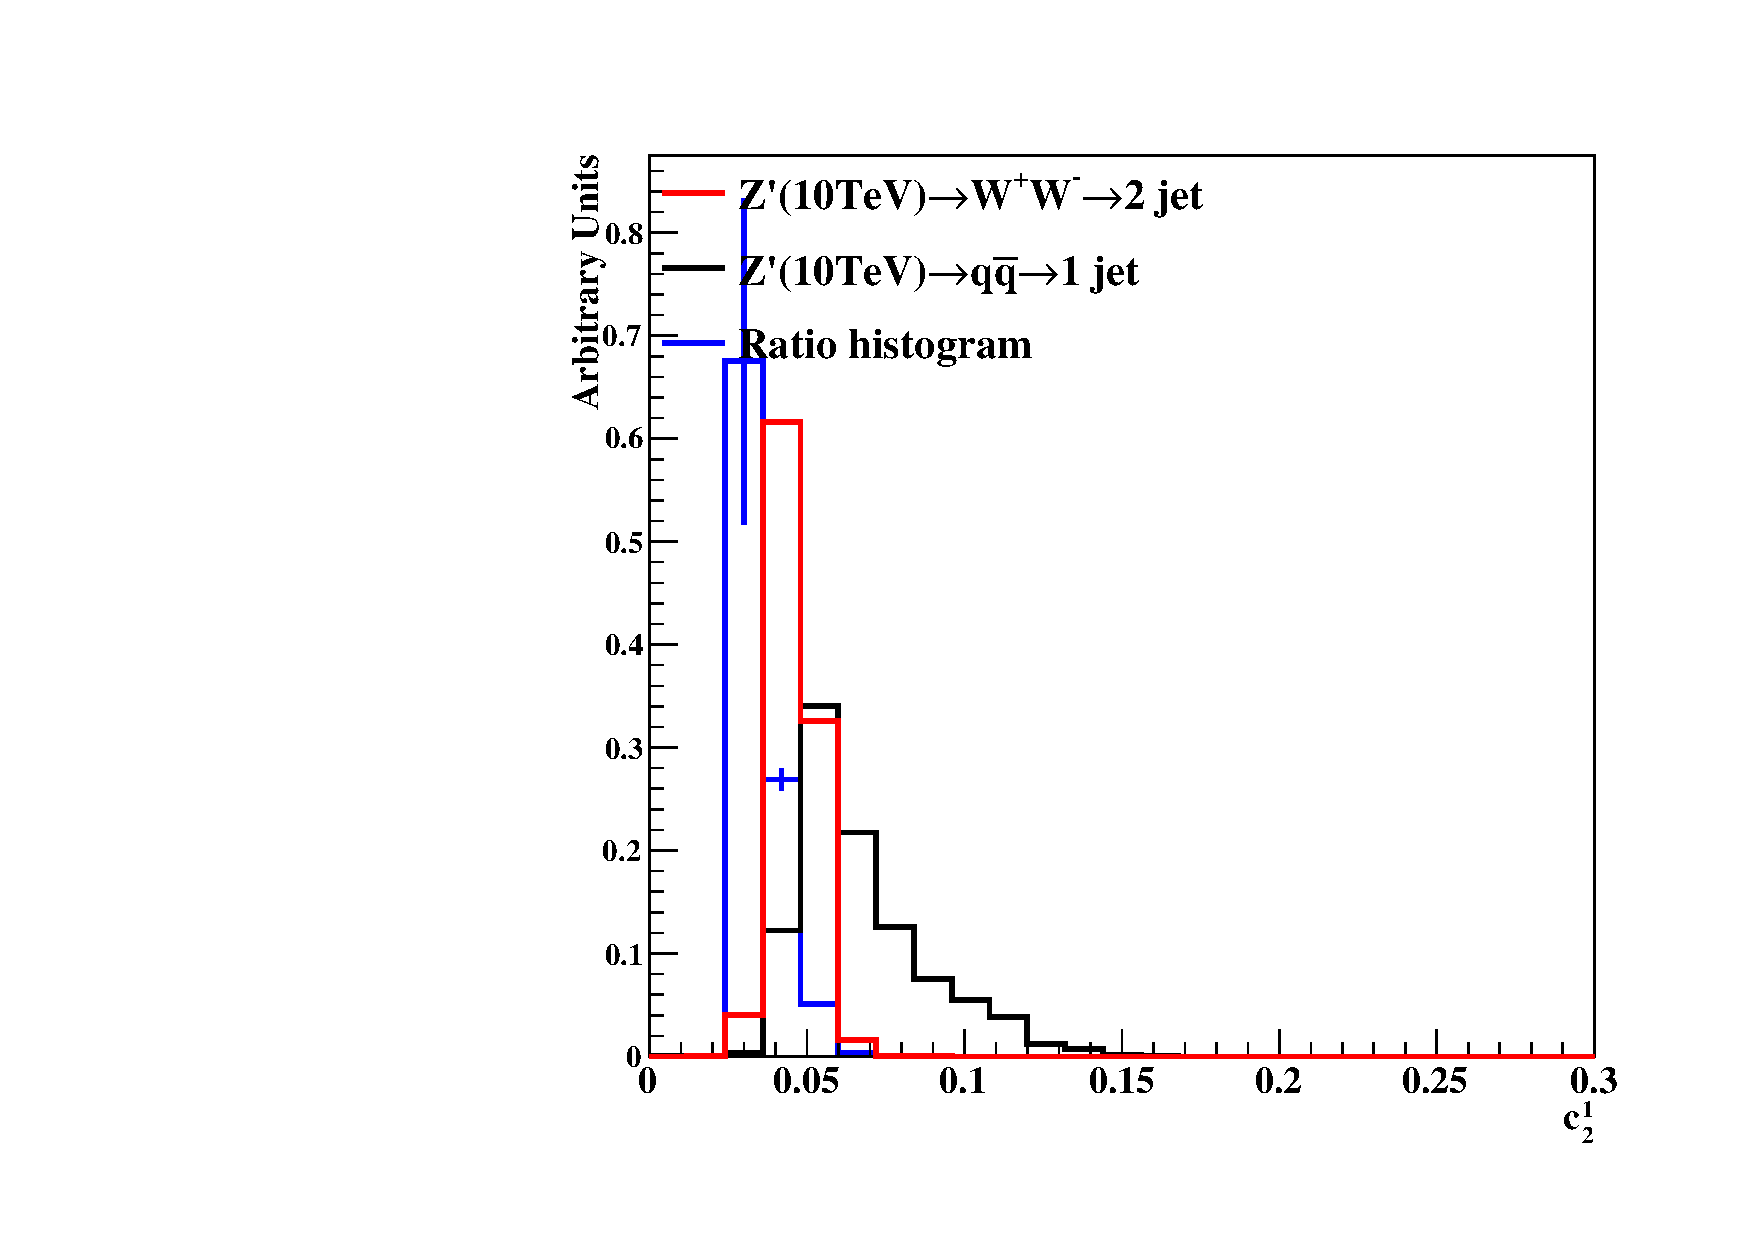
\includegraphics[width=0.22\textwidth]{figs/Rawhit_05GeV_009_c2b1_10tev_04_no_cut_25bins_Ratio.pdf}
   }
   \subfigure[20TeV at 5$\times$5(cm$\times$cm) in 0.5GeV] {
   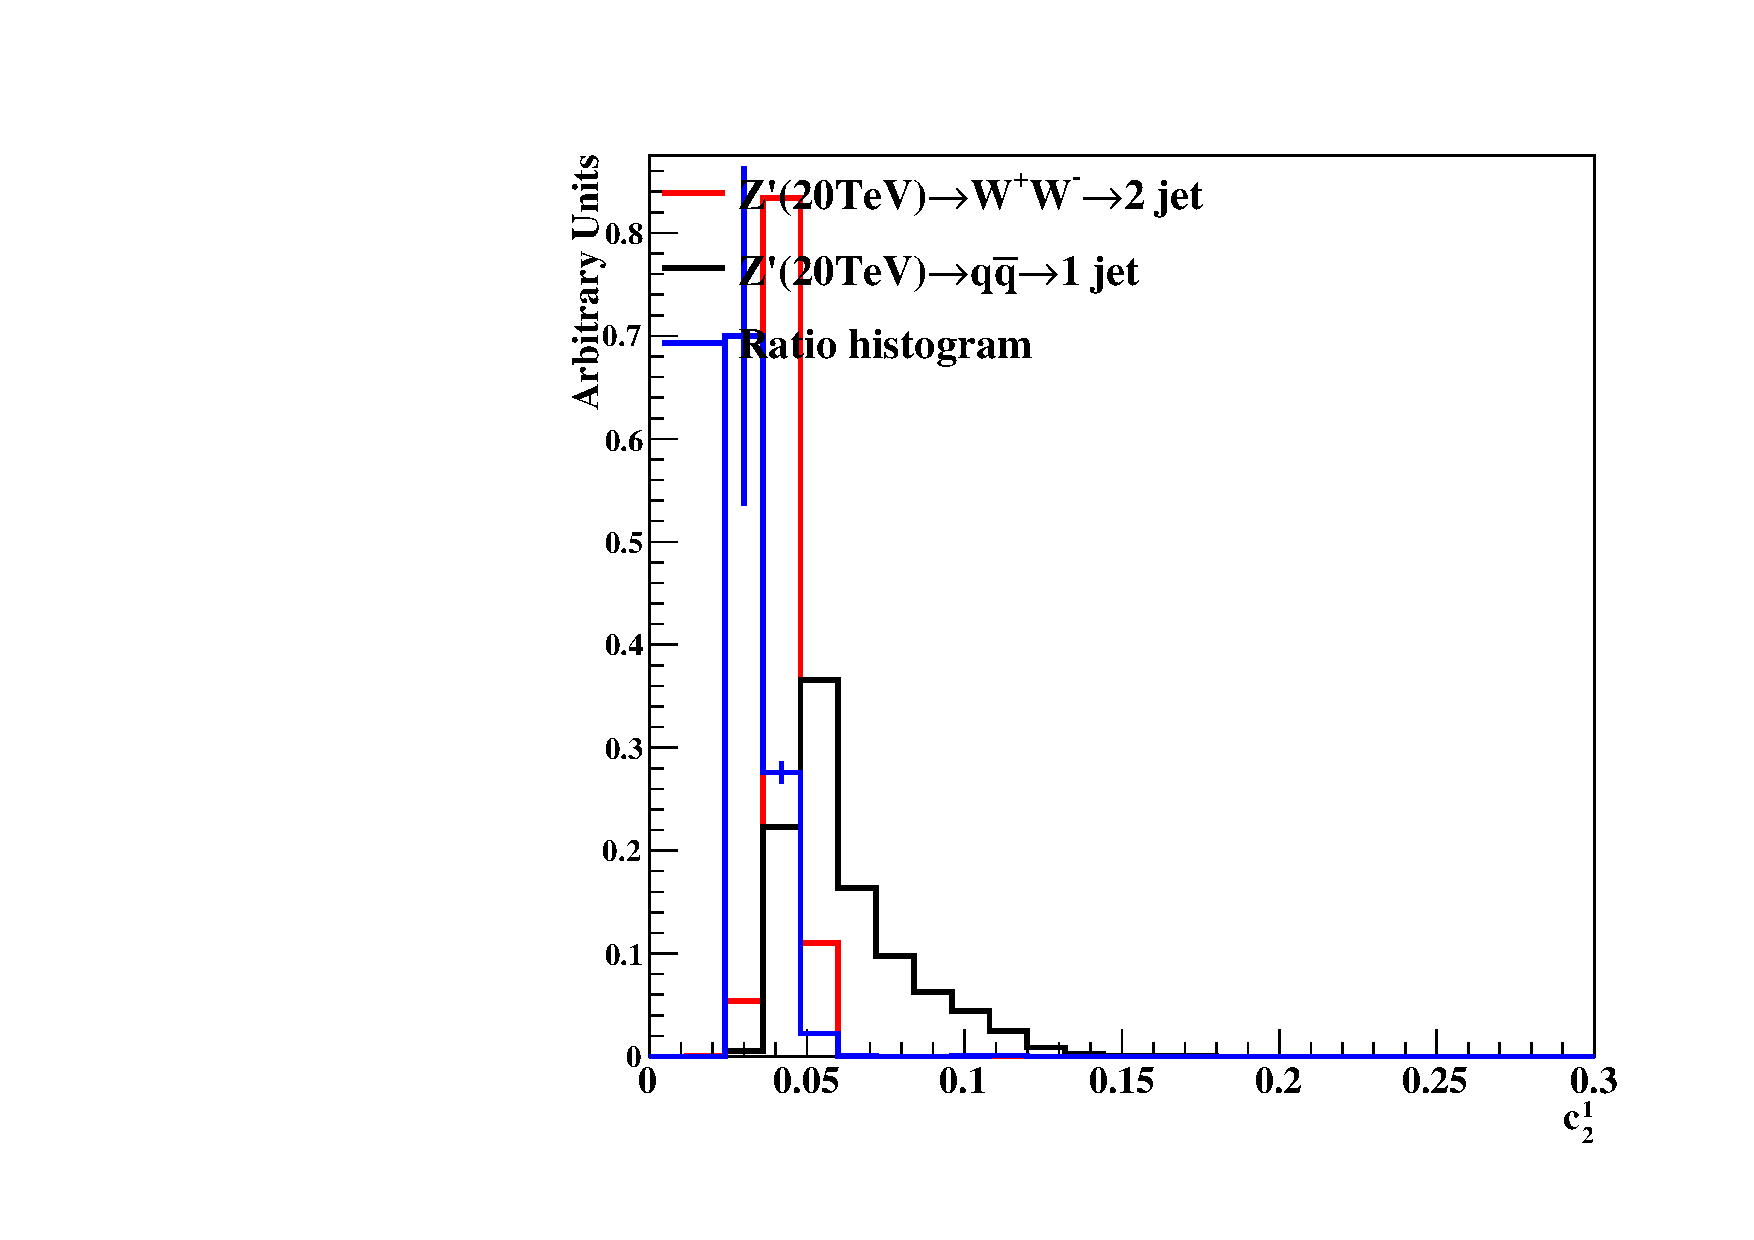
\includegraphics[width=0.22\textwidth]{figs/Rawhit_05GeV_009_c2b1_20tev_04_no_cut_25bins_Ratio.pdf}
   }
   \subfigure[40TeV at 5$\times$5(cm$\times$cm) in 0.5GeV] {
   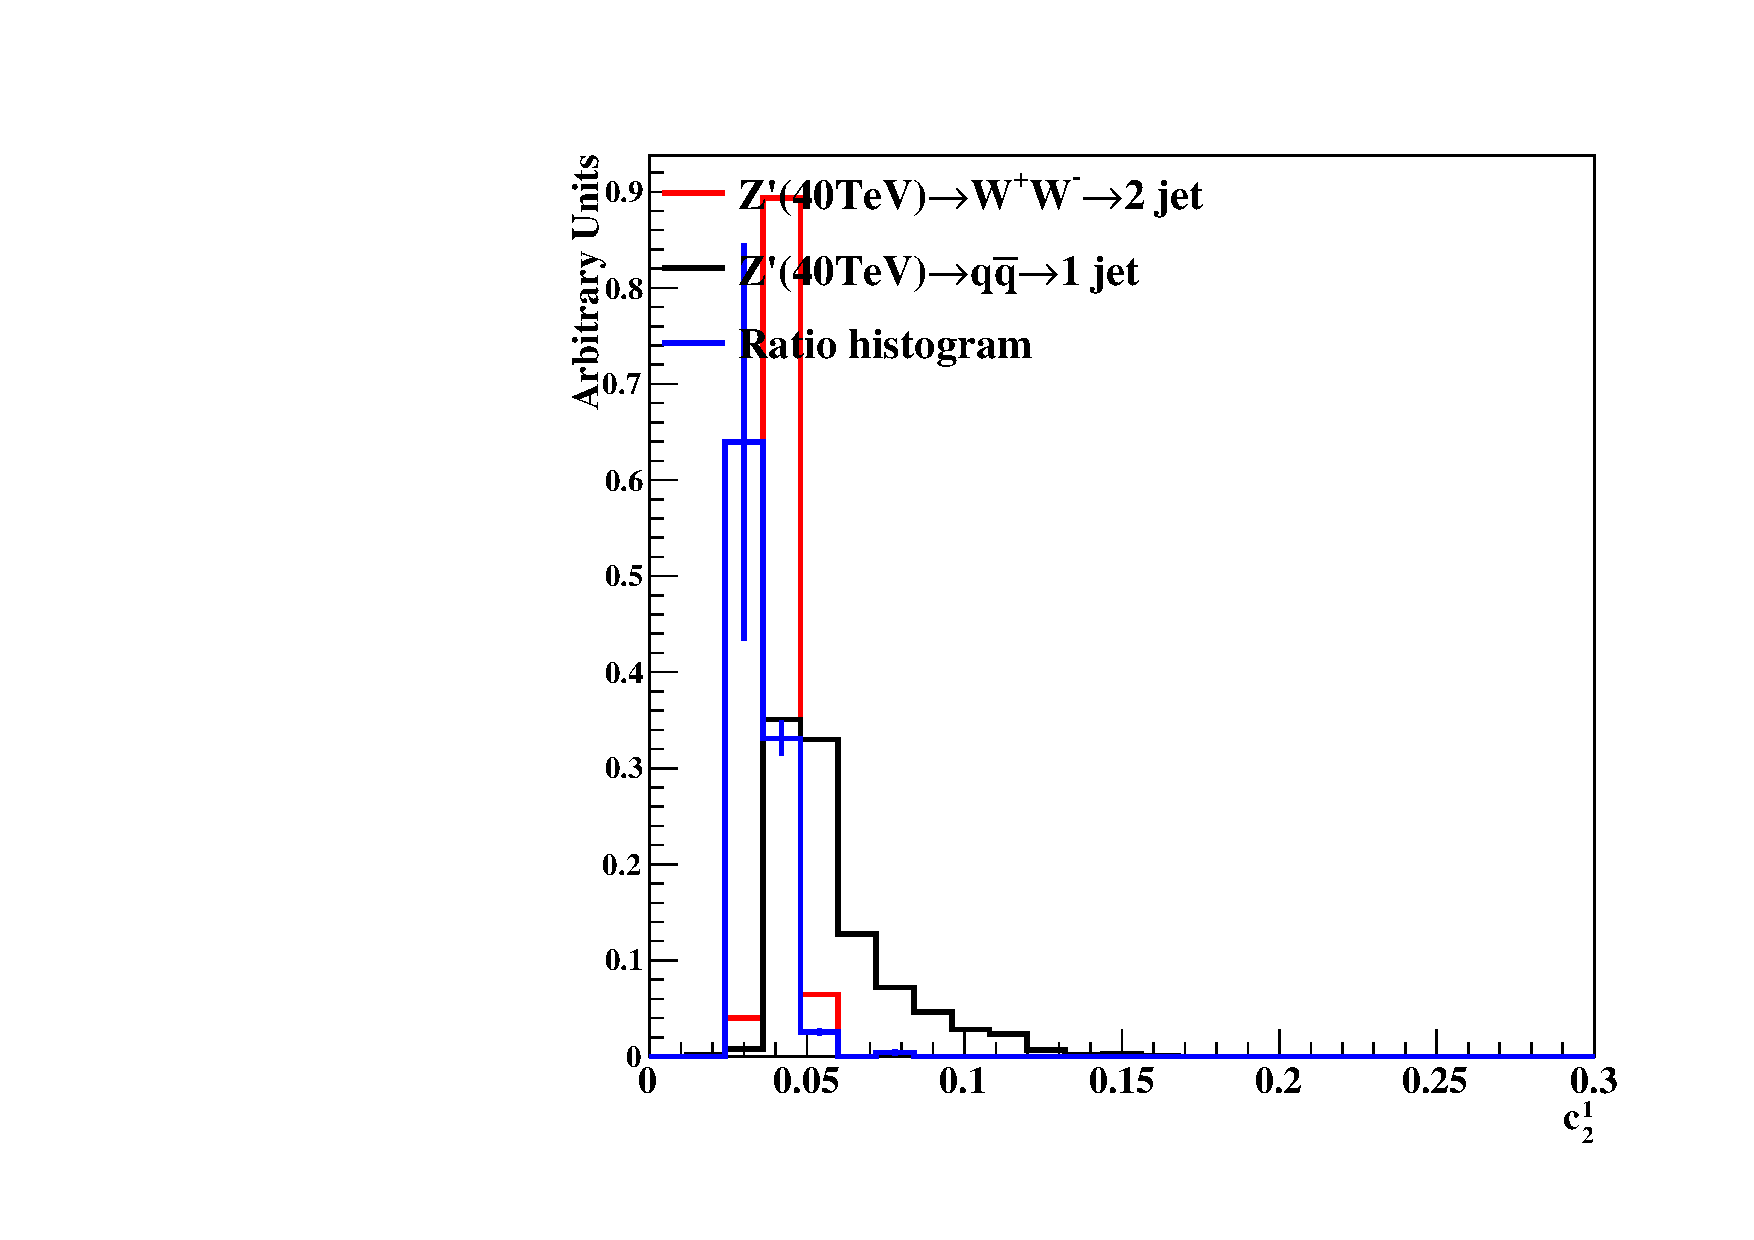
\includegraphics[width=0.22\textwidth]{figs/Rawhit_05GeV_009_c2b1_40tev_04_no_cut_25bins_Ratio.pdf}
   }
   \subfigure[5TeV at 1$\times$1(cm$\times$cm) in 0.5GeV] {
   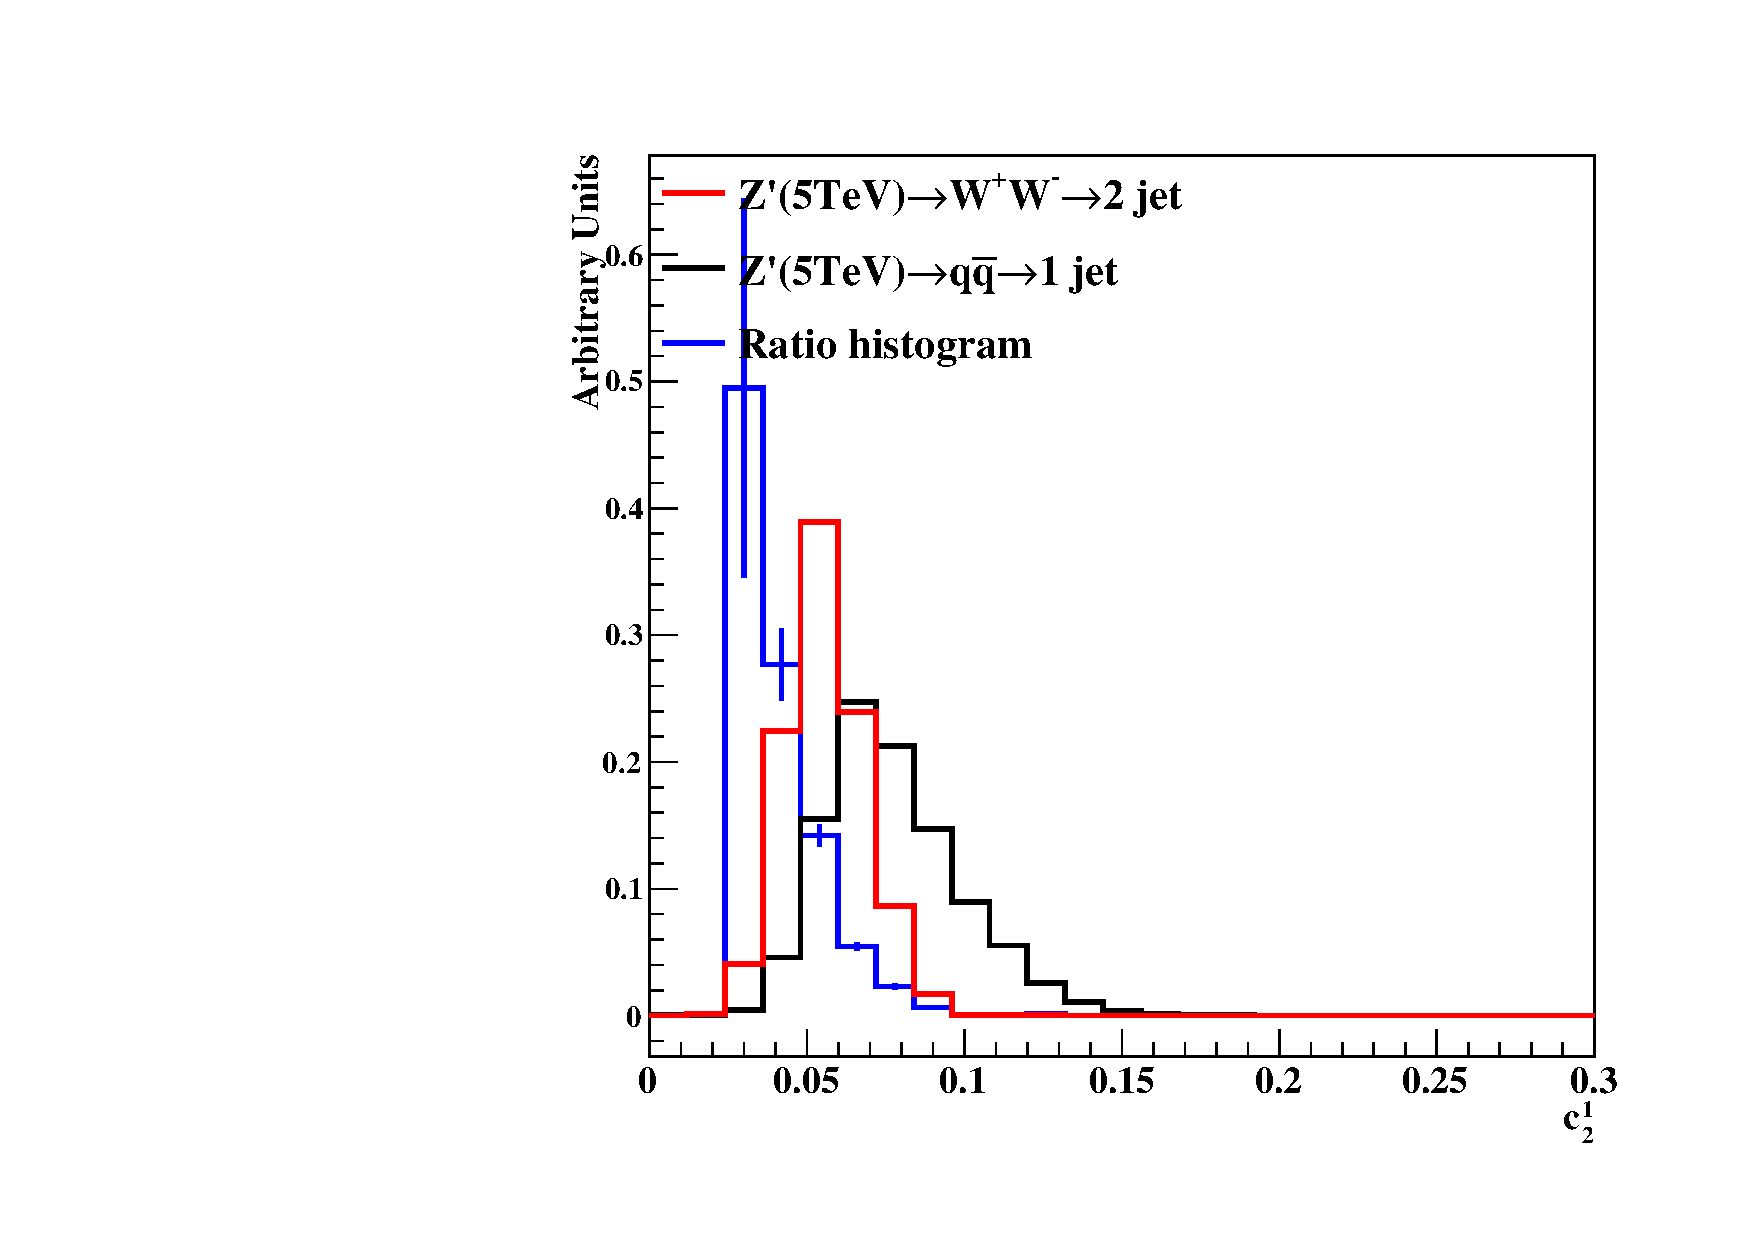
\includegraphics[width=0.22\textwidth]{figs/Rawhit_05GeV_012_c2b1_5tev_04_no_cut_25bins_Ratio.pdf}
   }
   \subfigure[10TeV at 1$\times$1(cm$\times$cm) in 0.5GeV] {
   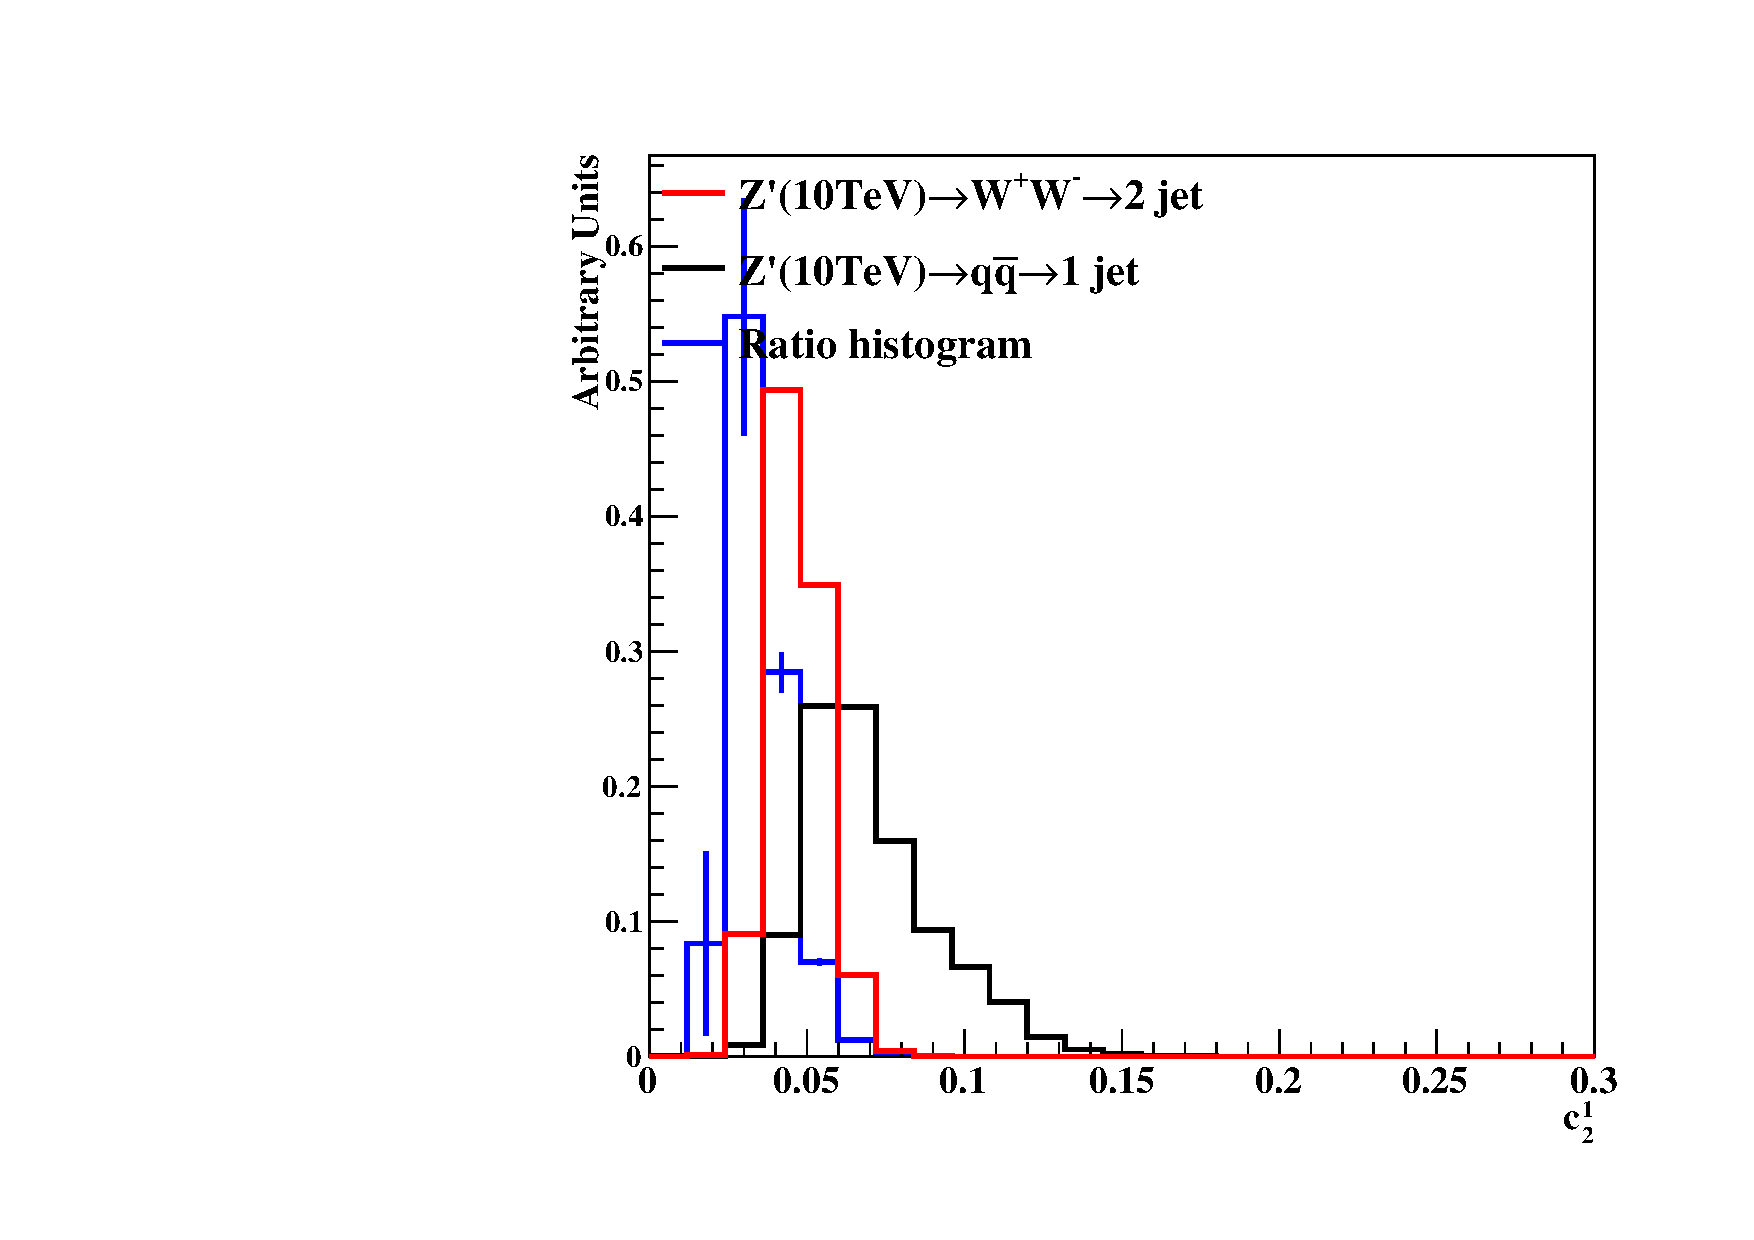
\includegraphics[width=0.22\textwidth]{figs/Rawhit_05GeV_012_c2b1_10tev_04_no_cut_25bins_Ratio.pdf}
   }
   \subfigure[20TeV at 1$\times$1(cm$\times$cm) in 0.5GeV] {
   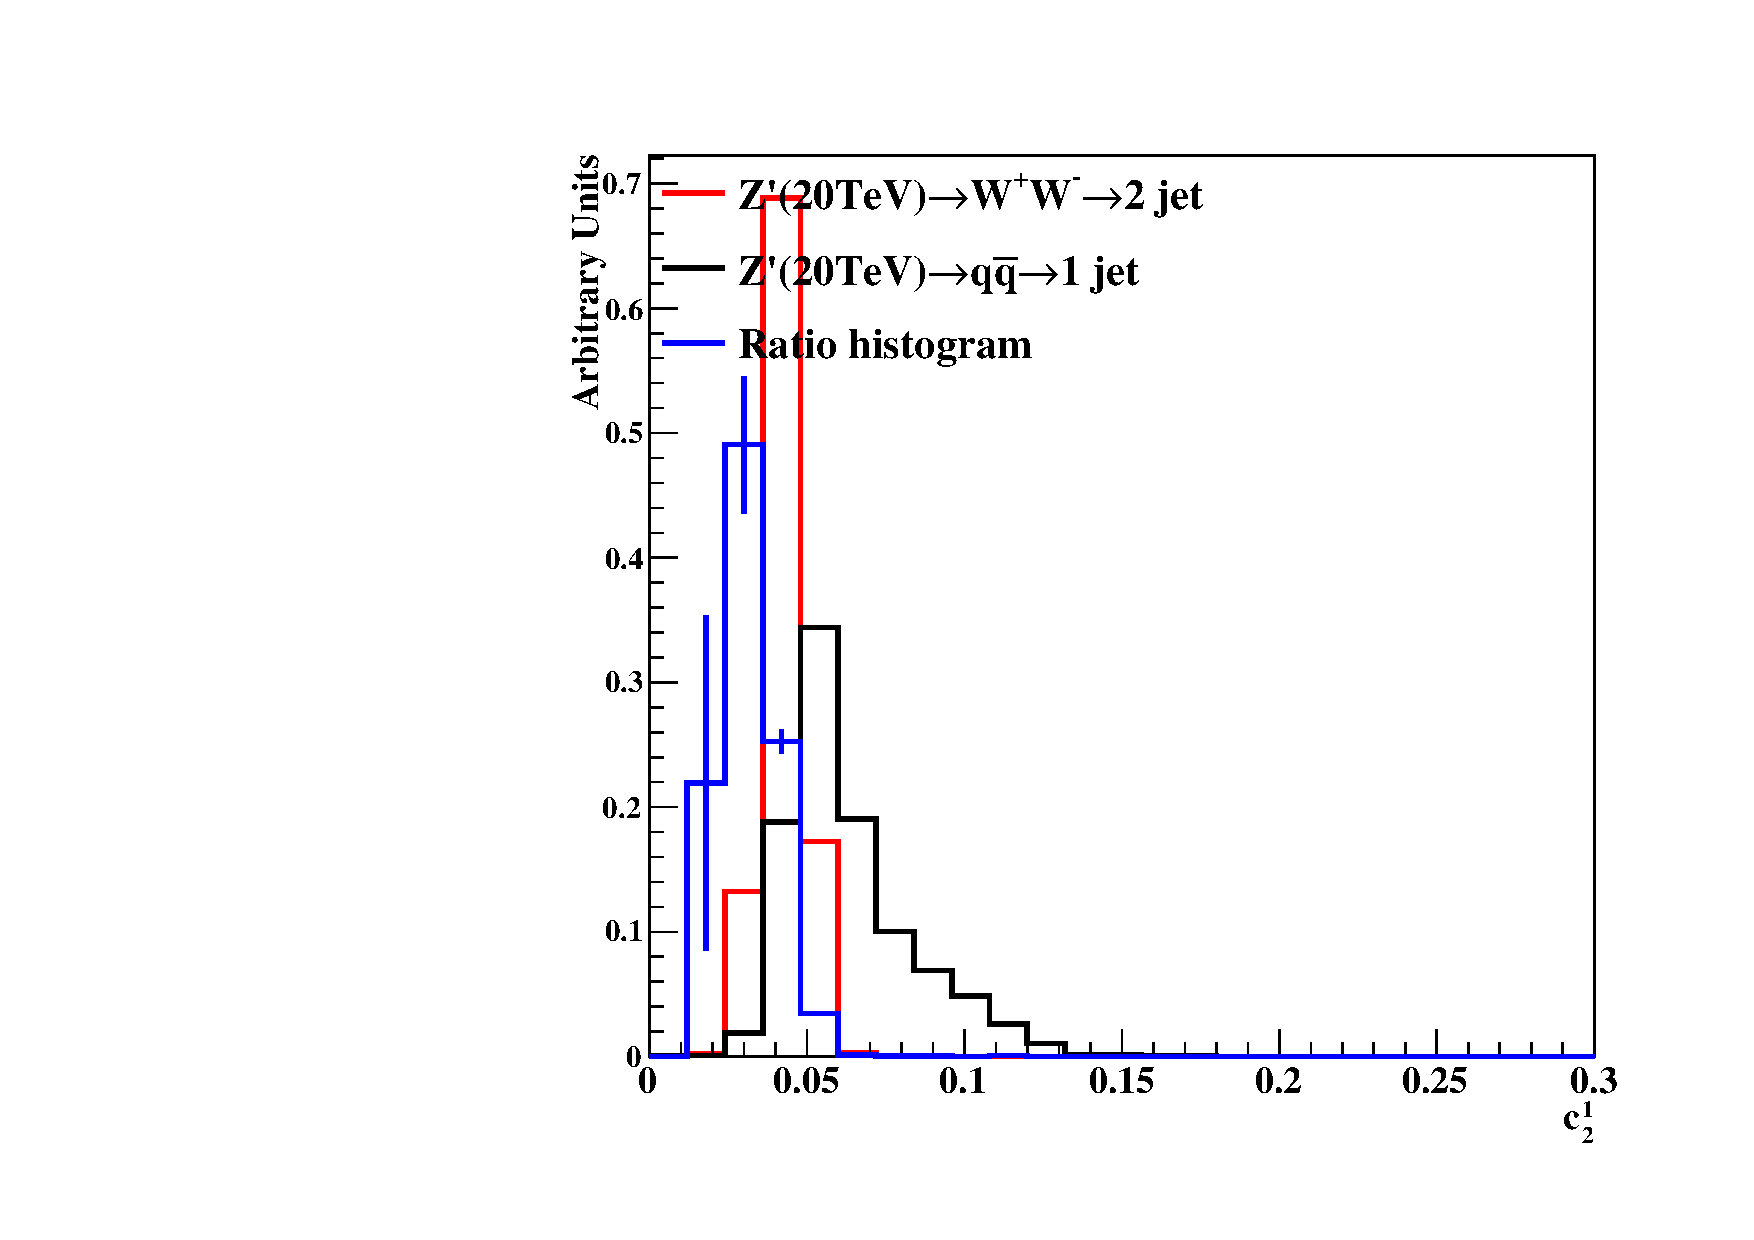
\includegraphics[width=0.22\textwidth]{figs/Rawhit_05GeV_012_c2b1_20tev_04_no_cut_25bins_Ratio.pdf}
   }
   \subfigure[40TeV at 1$\times$1(cm$\times$cm) in 0.5GeV] {
   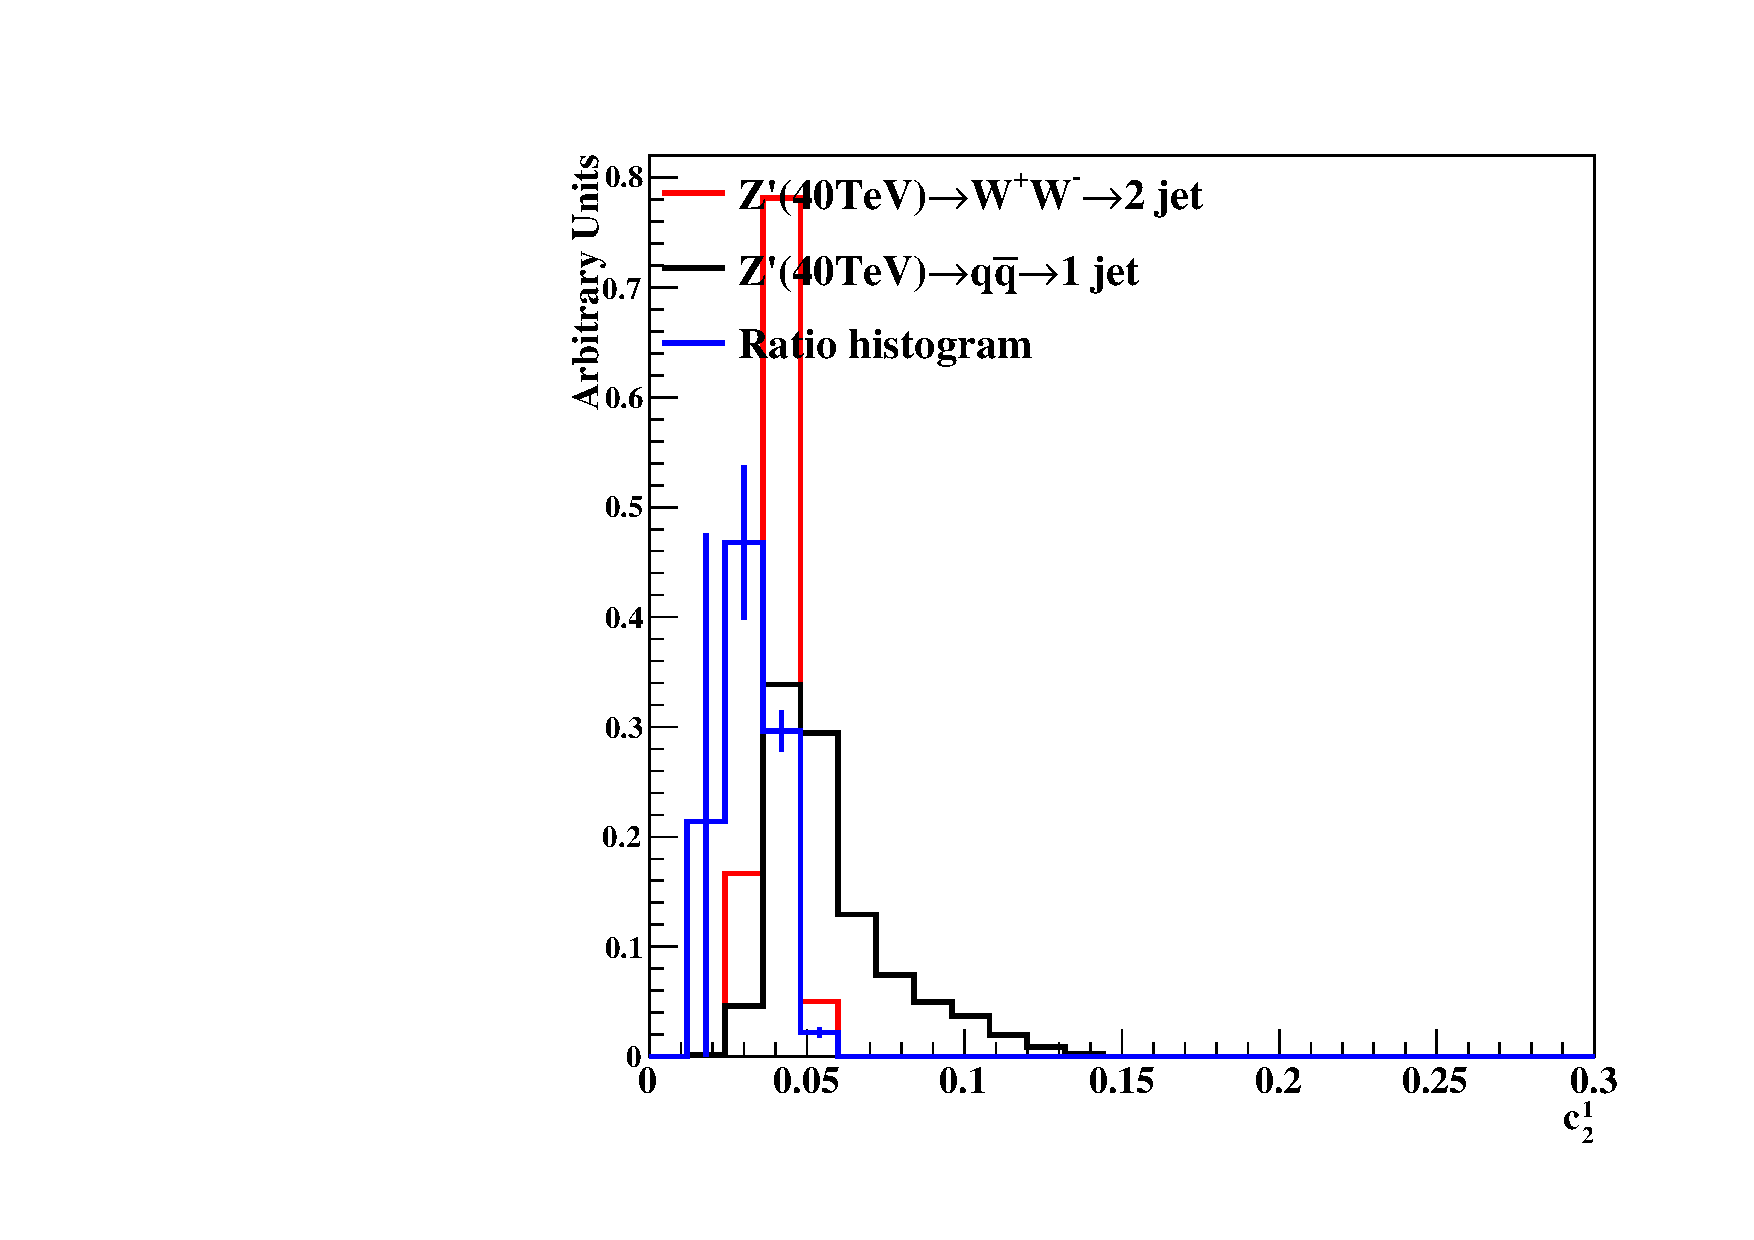
\includegraphics[width=0.22\textwidth]{figs/Rawhit_05GeV_012_c2b1_40tev_04_no_cut_25bins_Ratio.pdf}
   }\end{center}
\caption{Distributions of Mann-Whitney value U in 5, 10, 20, 40TeV energy collision for c2b1 in different detector sizes WithoutCut. Cell Size in 20$\times$20, 5$\times$5, and 1$\times$1(cm$\times$cm) are shown here.}
\label{fig:cluster_c2b1_tau32}
\end{figure}

\begin{figure}
\begin{center}
   \subfigure[5 TeV using Rawhit 0.5GeV cut method with New2 no cut Method] {
   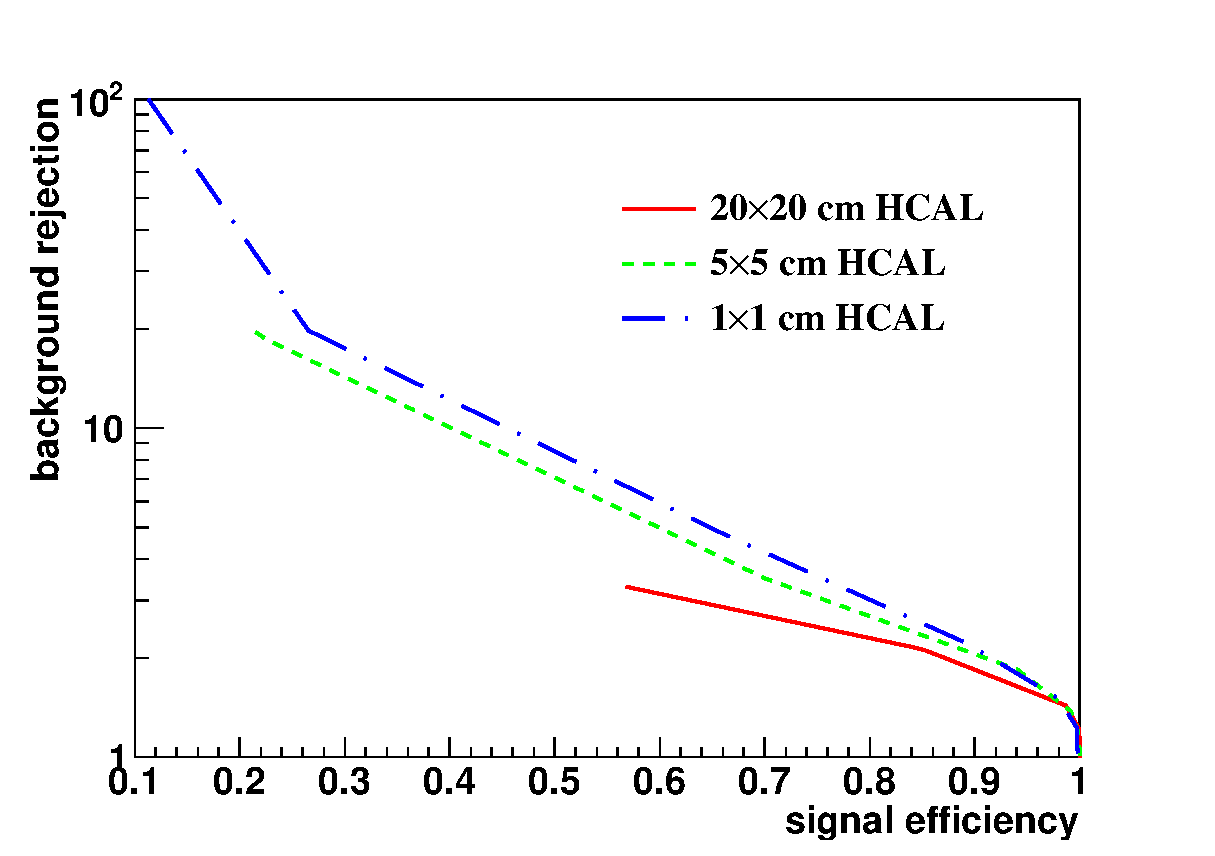
\includegraphics[width=0.43\textwidth]{figs/Rawhit_05GeV_c2b1_5tev_eff_1_New2_no_cut_25bins.eps}\hfill
   }
   \subfigure[10 TeV using Rawhit 0.5GeV cut method with New2 no cut Method] {
   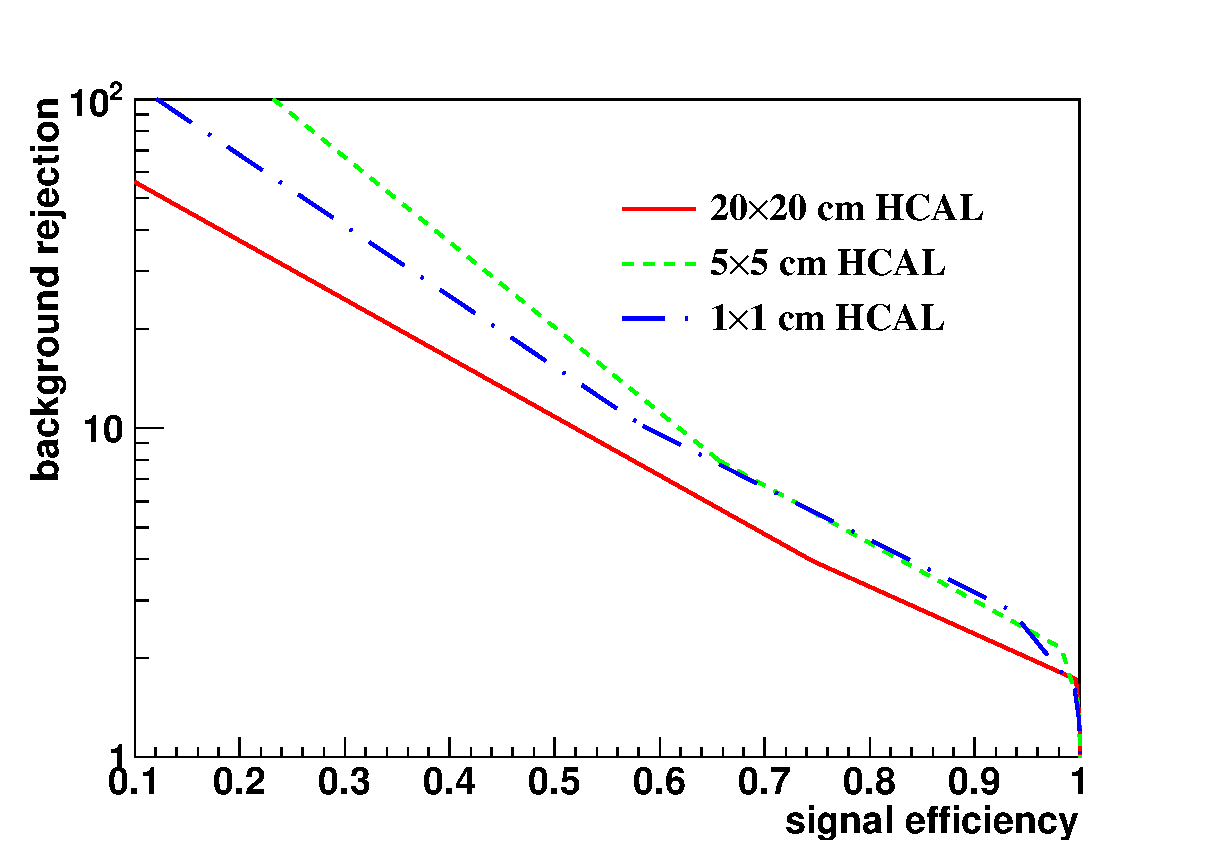
\includegraphics[width=0.43\textwidth]{figs/Rawhit_05GeV_c2b1_10tev_eff_1_New2_no_cut_25bins.eps}
   }
   \subfigure[20 TeV using Rawhit 0.5GeV cut method with New2 no cut Method] {
   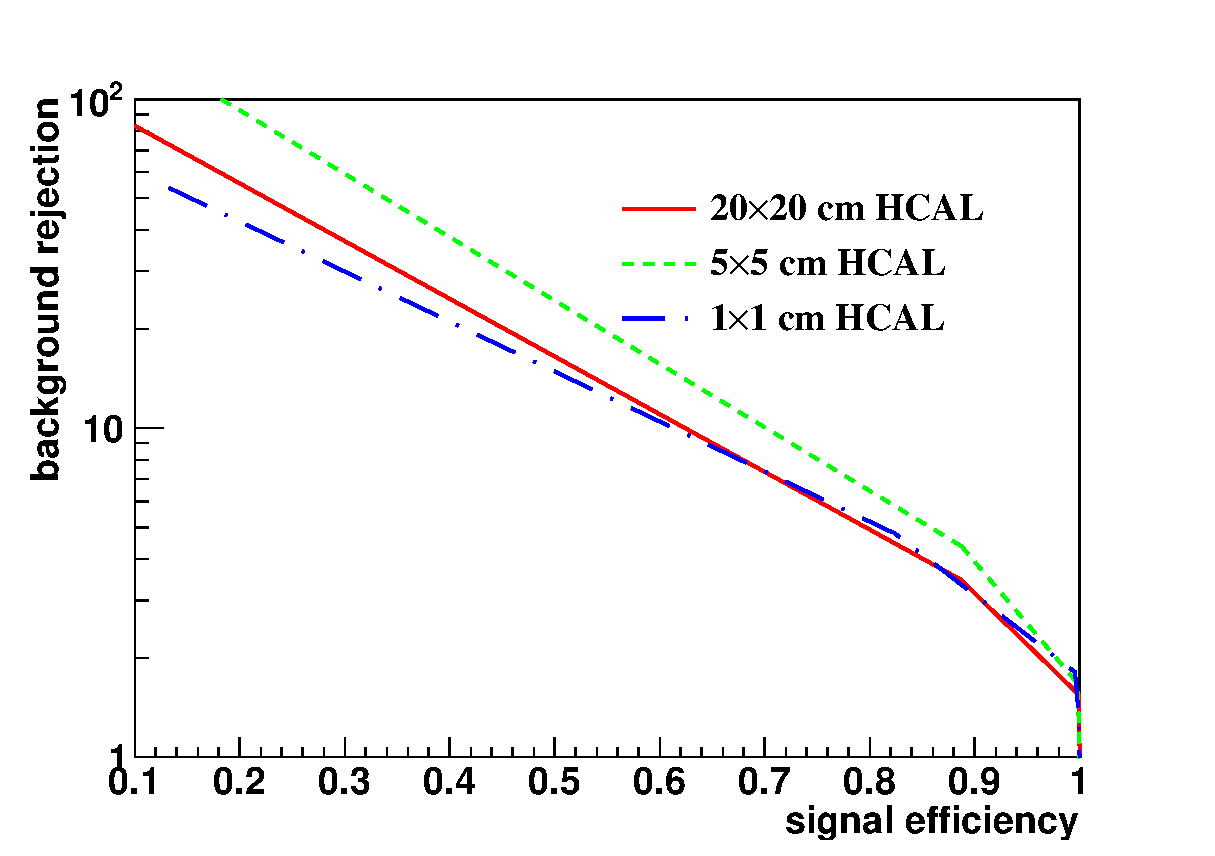
\includegraphics[width=0.43\textwidth]{figs/Rawhit_05GeV_c2b1_20tev_eff_1_New2_no_cut_25bins.eps}
   }
   \subfigure[40 TeV using Rawhit 0.5GeV cut method with New2 no cut Method] {
   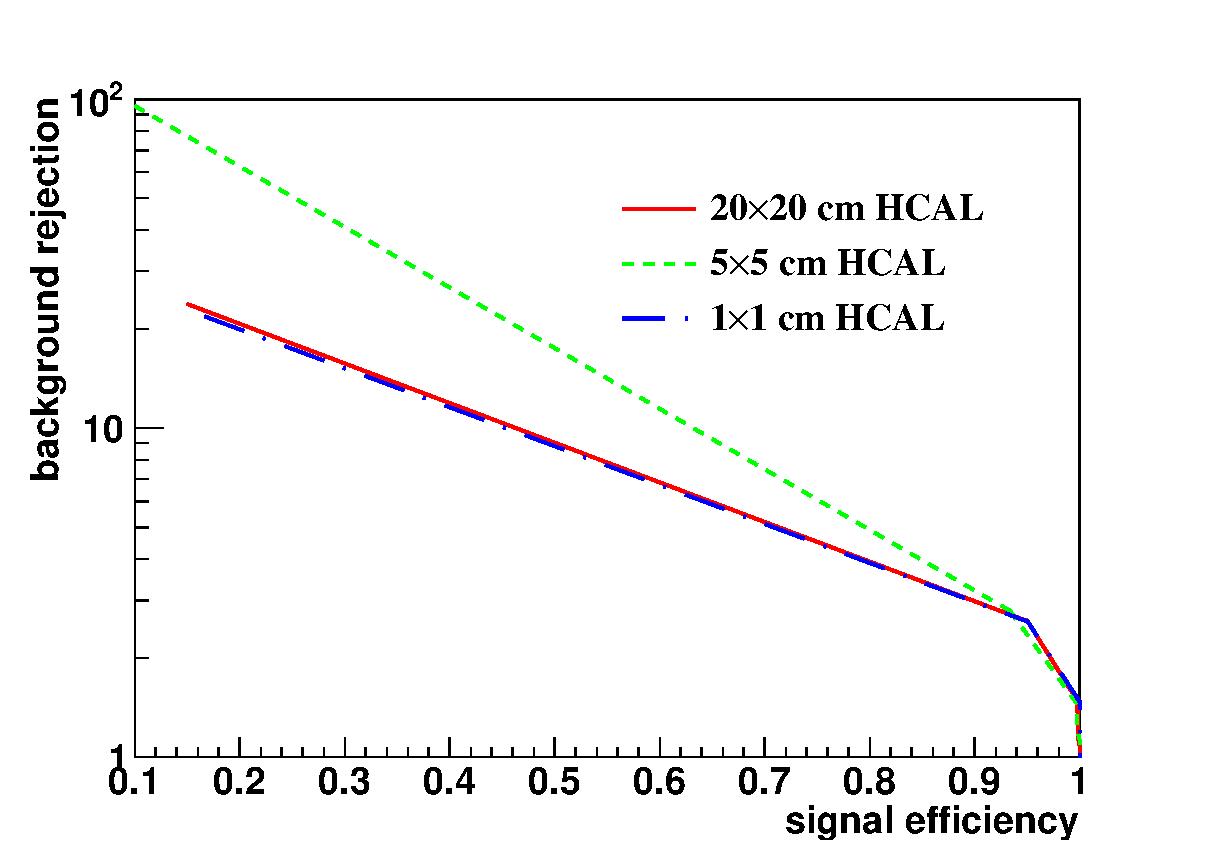
\includegraphics[width=0.43\textwidth]{figs/Rawhit_05GeV_c2b1_40tev_eff_1_New2_no_cut_25bins.eps}
   }
\end{center}
\caption{Signal efficiency versus background rejection rate using c2b1 WithoutCut.The energies of collision at (a)5, (b)10, (c)20, (d)40TeV are shown here. In each picture, the three ROC curves correspond to different detector sizes.}
\label{fig:cluster_c2b1}
\end{figure}

%25bins
\begin{figure}
\begin{center}
   \subfigure[5TeV at 20$\times$20(cm$\times$cm) in 0.5GeV] {
   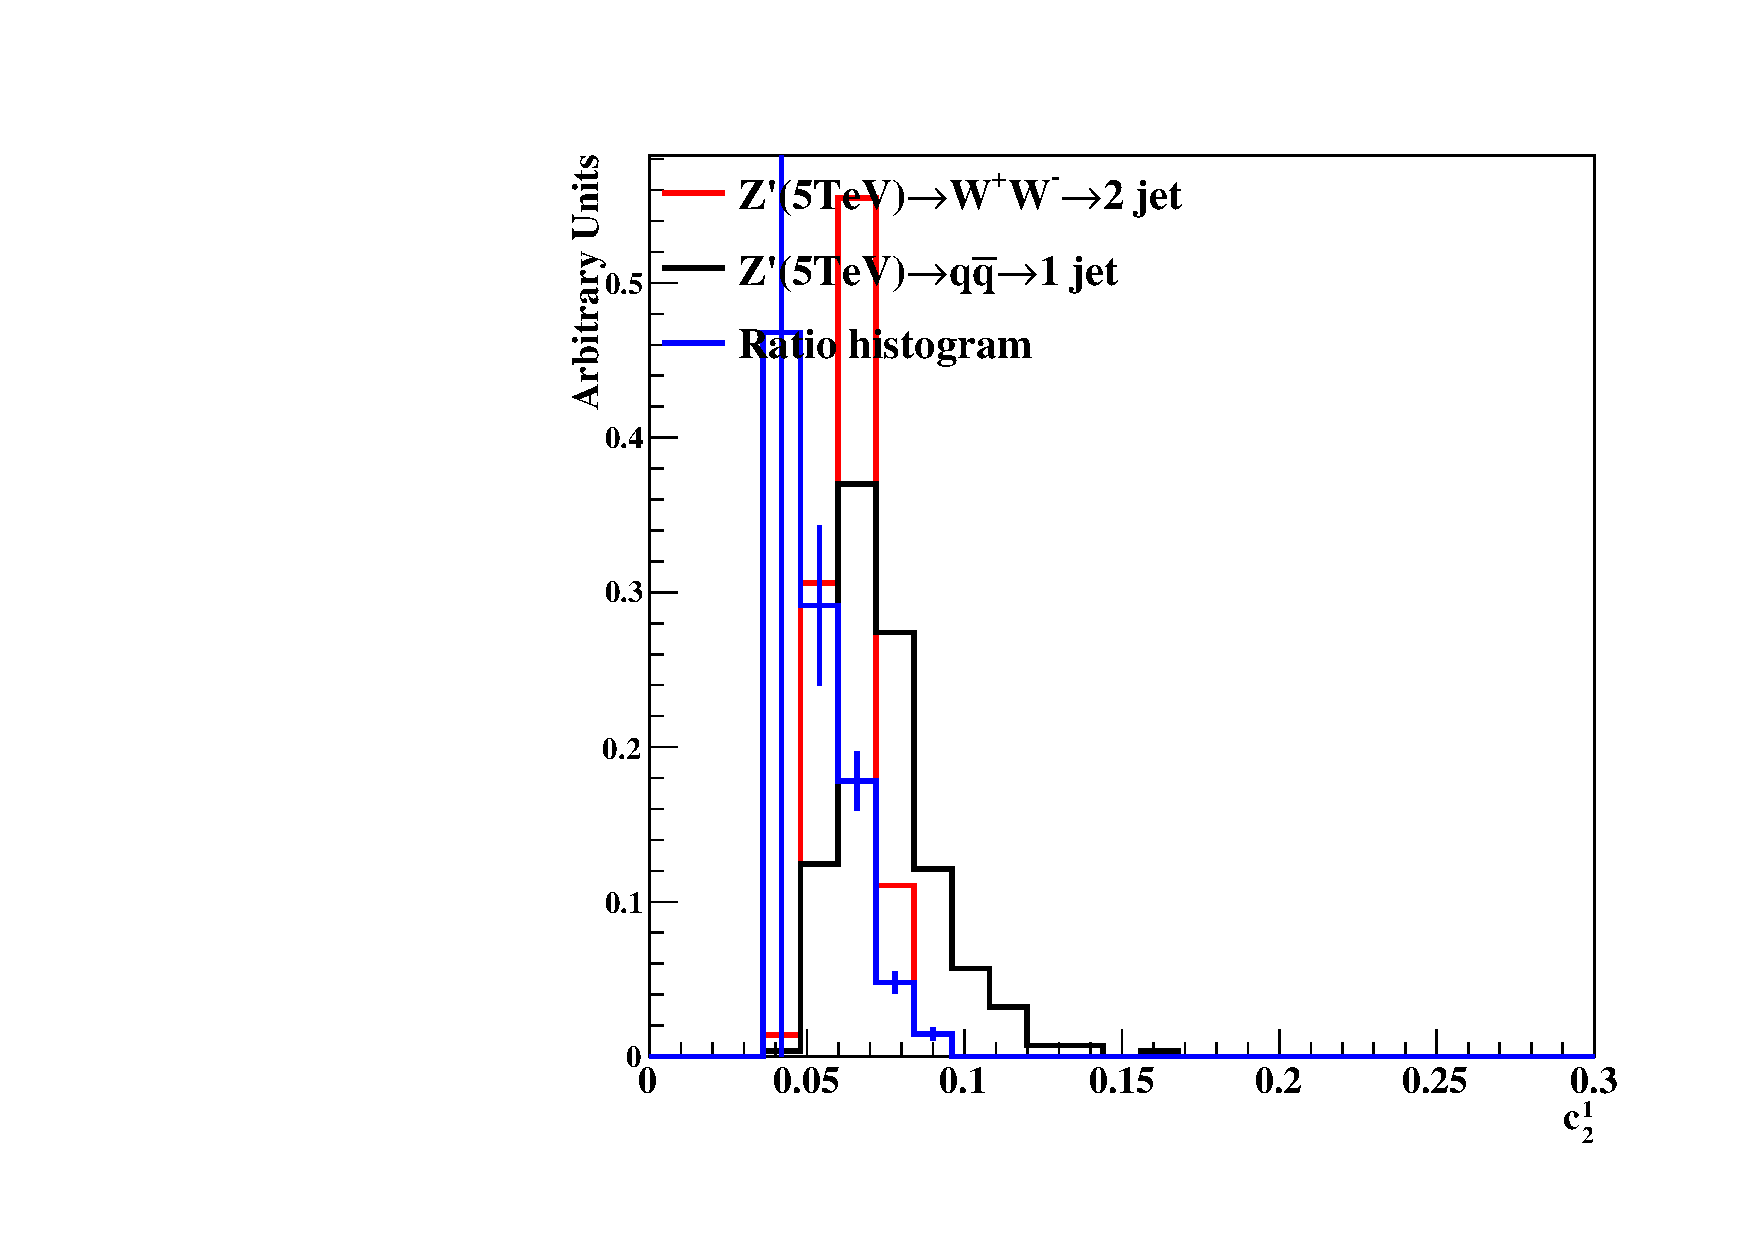
\includegraphics[width=0.22\textwidth]{figs/Rawhit_05GeV_010_c2b1_5tev_04_after_cut_25bins_Ratio.pdf}\hfill
   }
   \subfigure[10TeV at 20$\times$20(cm$\times$cm) in 0.5GeV] {
   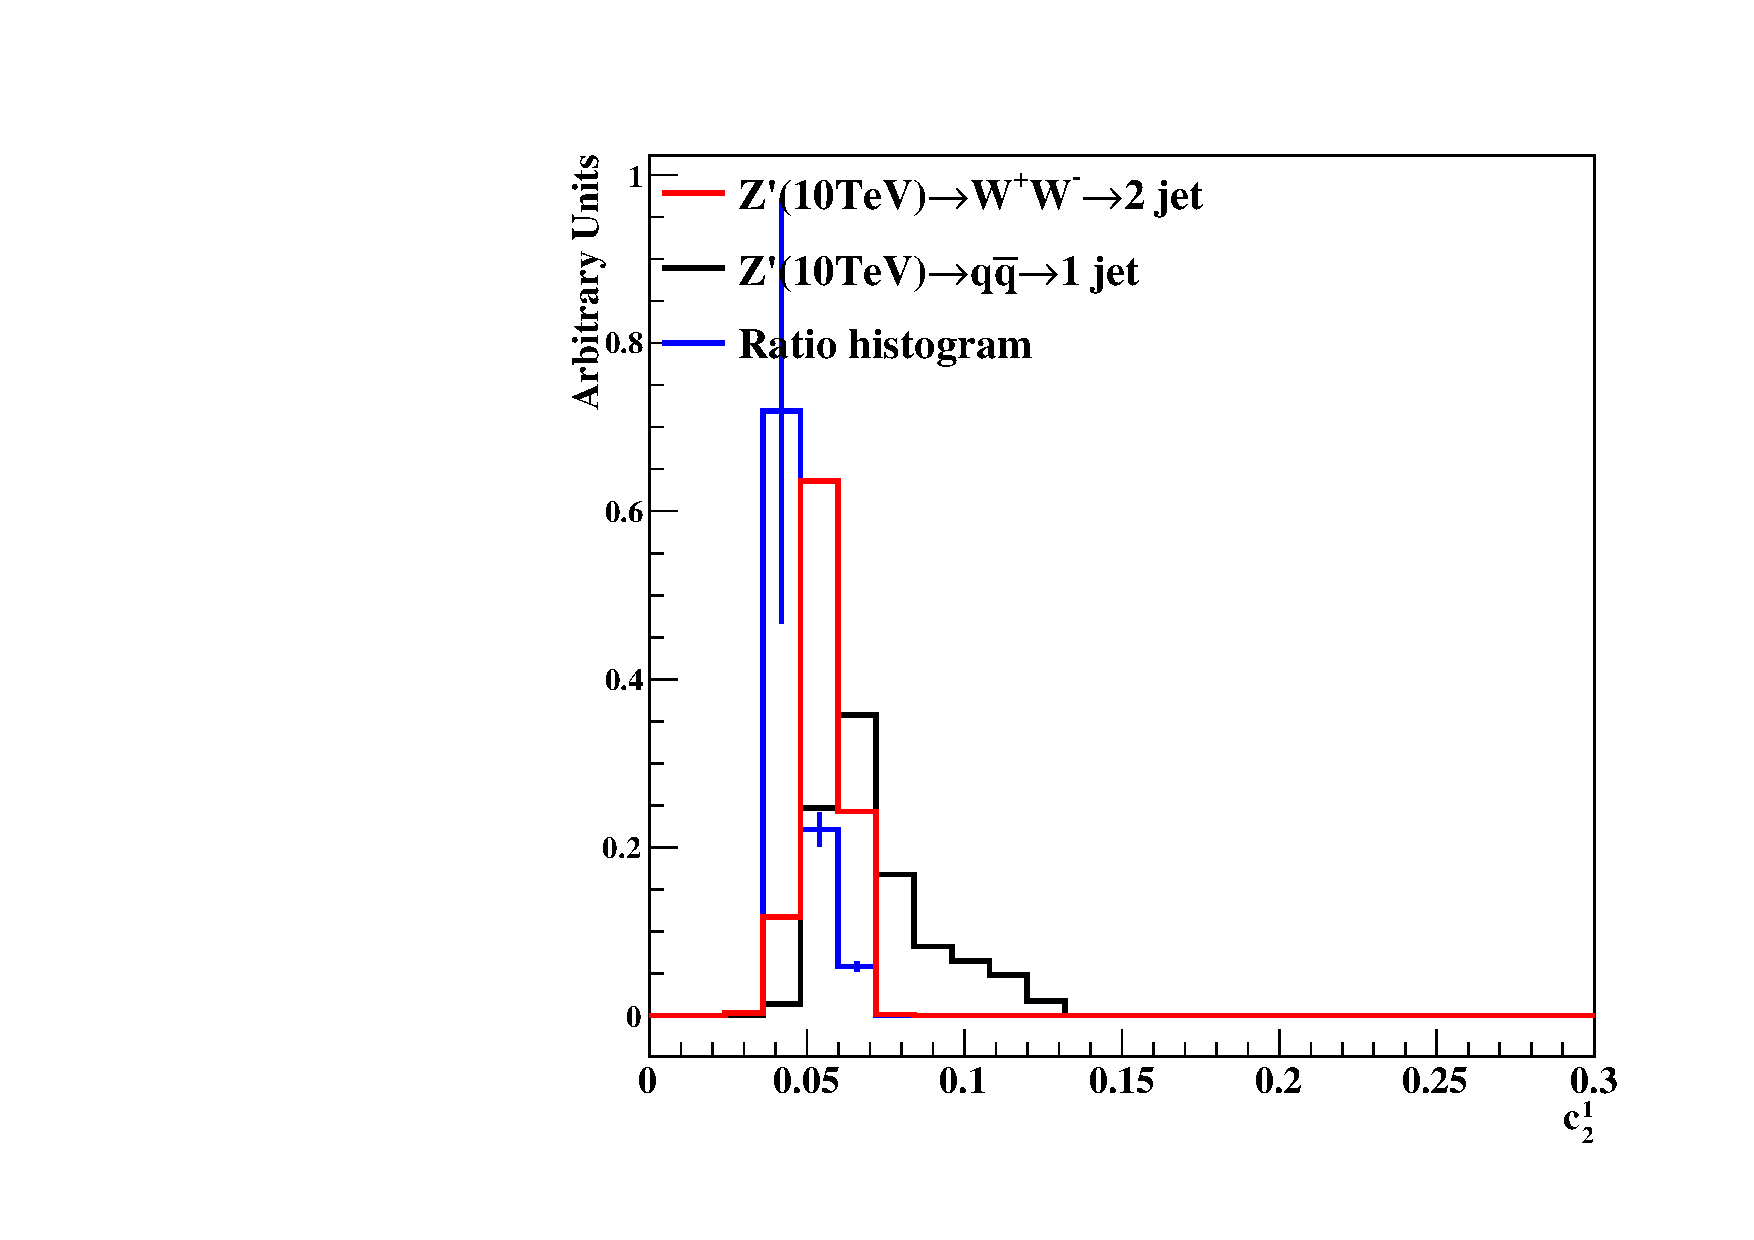
\includegraphics[width=0.22\textwidth]{figs/Rawhit_05GeV_010_c2b1_10tev_04_after_cut_25bins_Ratio.pdf}
   }
   \subfigure[20TeV at 20$\times$20(cm$\times$cm) in 0.5GeV] {
   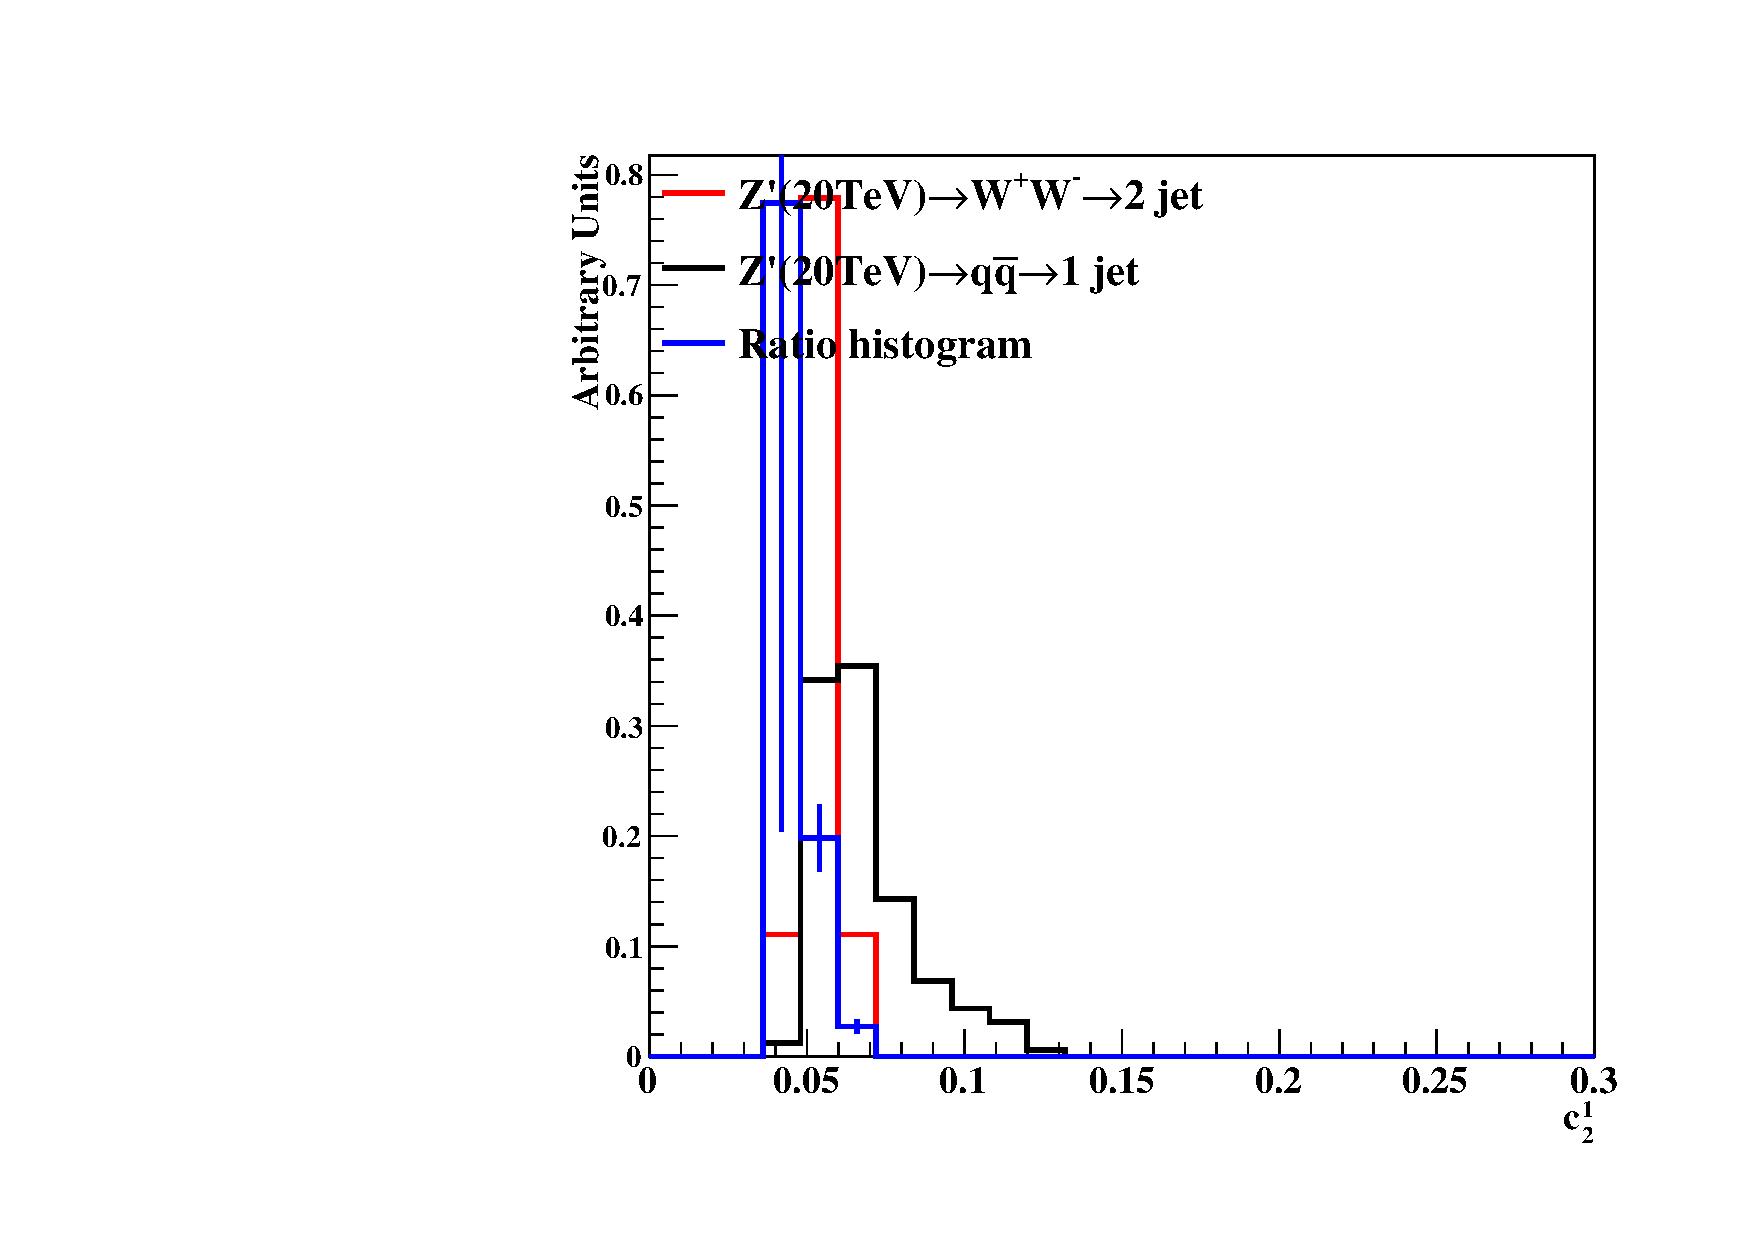
\includegraphics[width=0.22\textwidth]{figs/Rawhit_05GeV_010_c2b1_20tev_04_after_cut_25bins_Ratio.pdf}
   }
   \subfigure[40TeV at 20$\times$20(cm$\times$cm) in 0.5GeV] {
   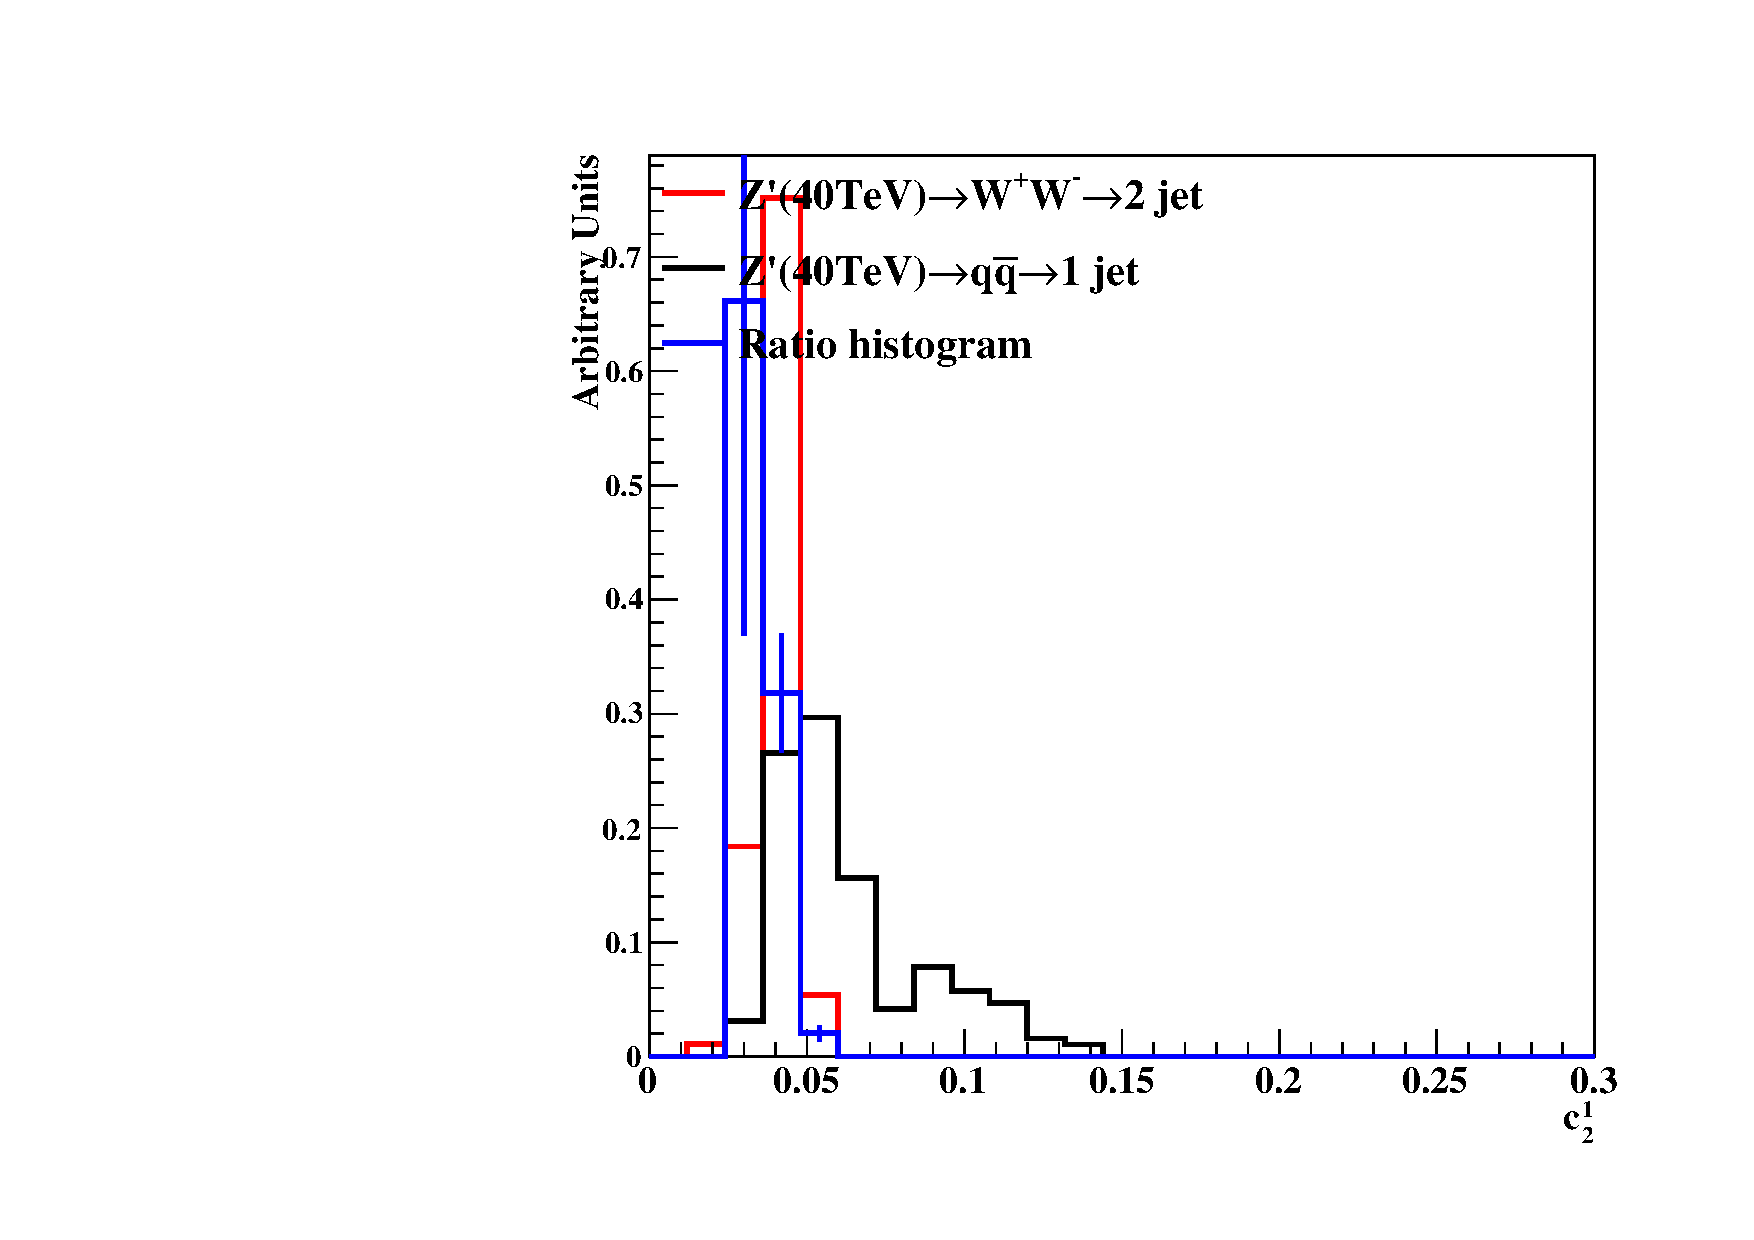
\includegraphics[width=0.22\textwidth]{figs/Rawhit_05GeV_010_c2b1_40tev_04_after_cut_25bins_Ratio.pdf}
   }
   \subfigure[5TeV at 5$\times$5(cm$\times$cm) in 0.5GeV] {
   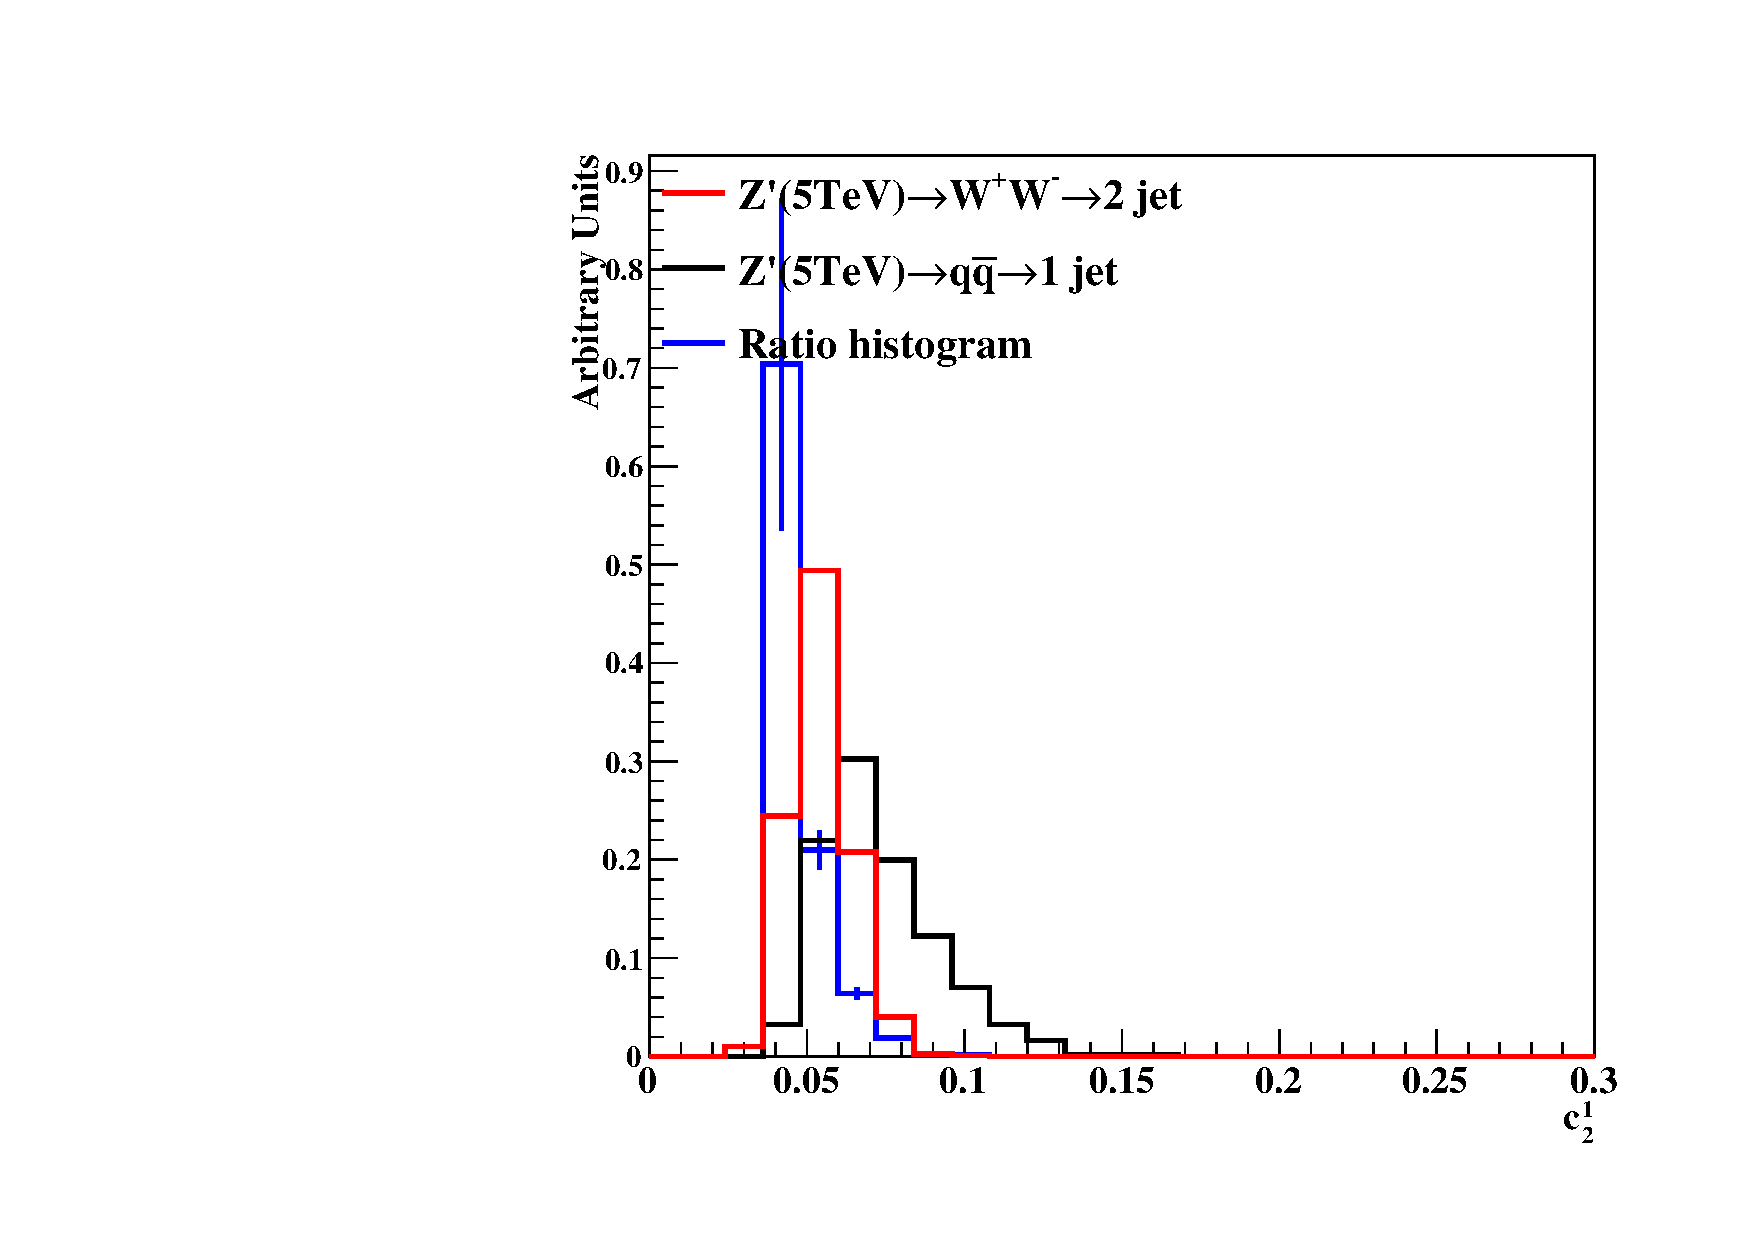
\includegraphics[width=0.22\textwidth]{figs/Rawhit_05GeV_009_c2b1_5tev_04_after_cut_25bins_Ratio.pdf}
   }
   \subfigure[10TeV at 5$\times$5(cm$\times$cm) in 0.5GeV] {
   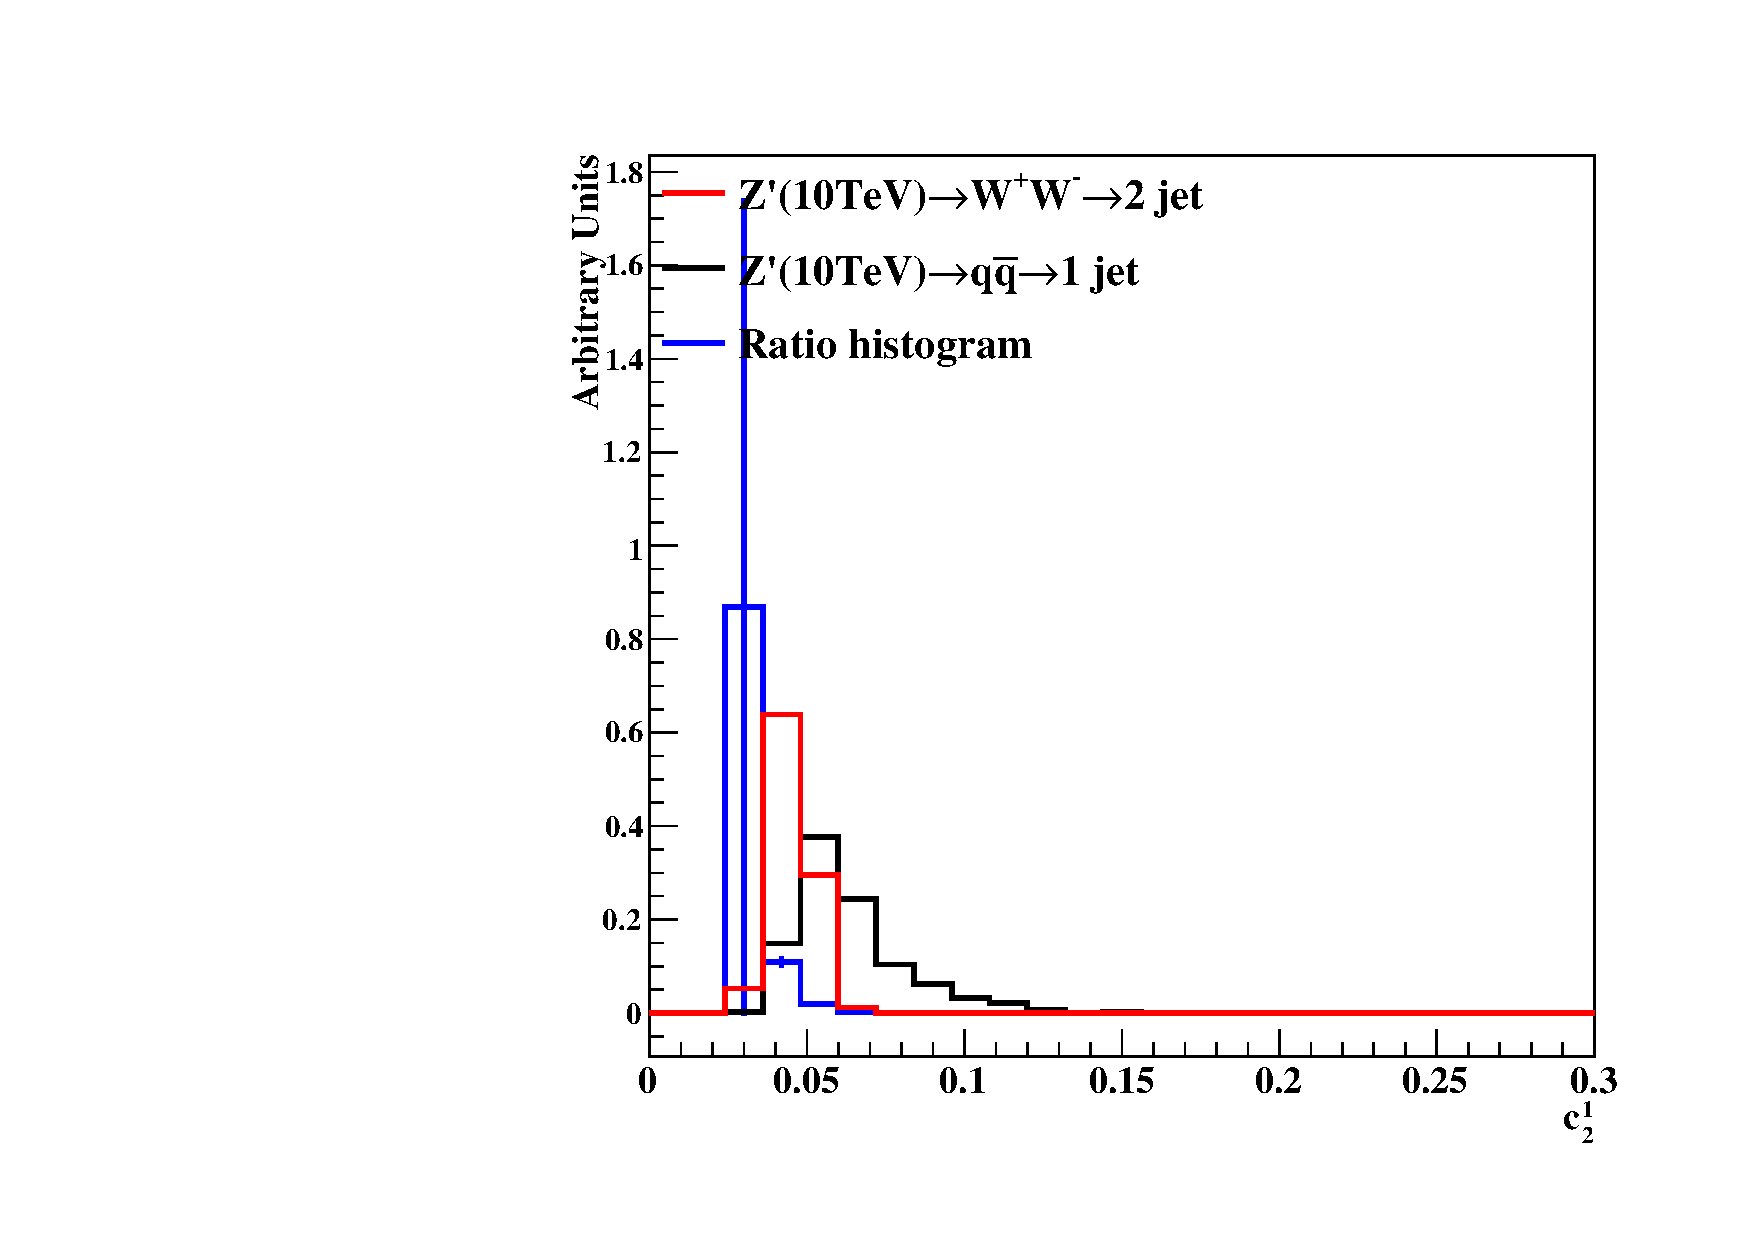
\includegraphics[width=0.22\textwidth]{figs/Rawhit_05GeV_009_c2b1_10tev_04_after_cut_25bins_Ratio.pdf}
   }
   \subfigure[20TeV at 5$\times$5(cm$\times$cm) in 0.5GeV] {
   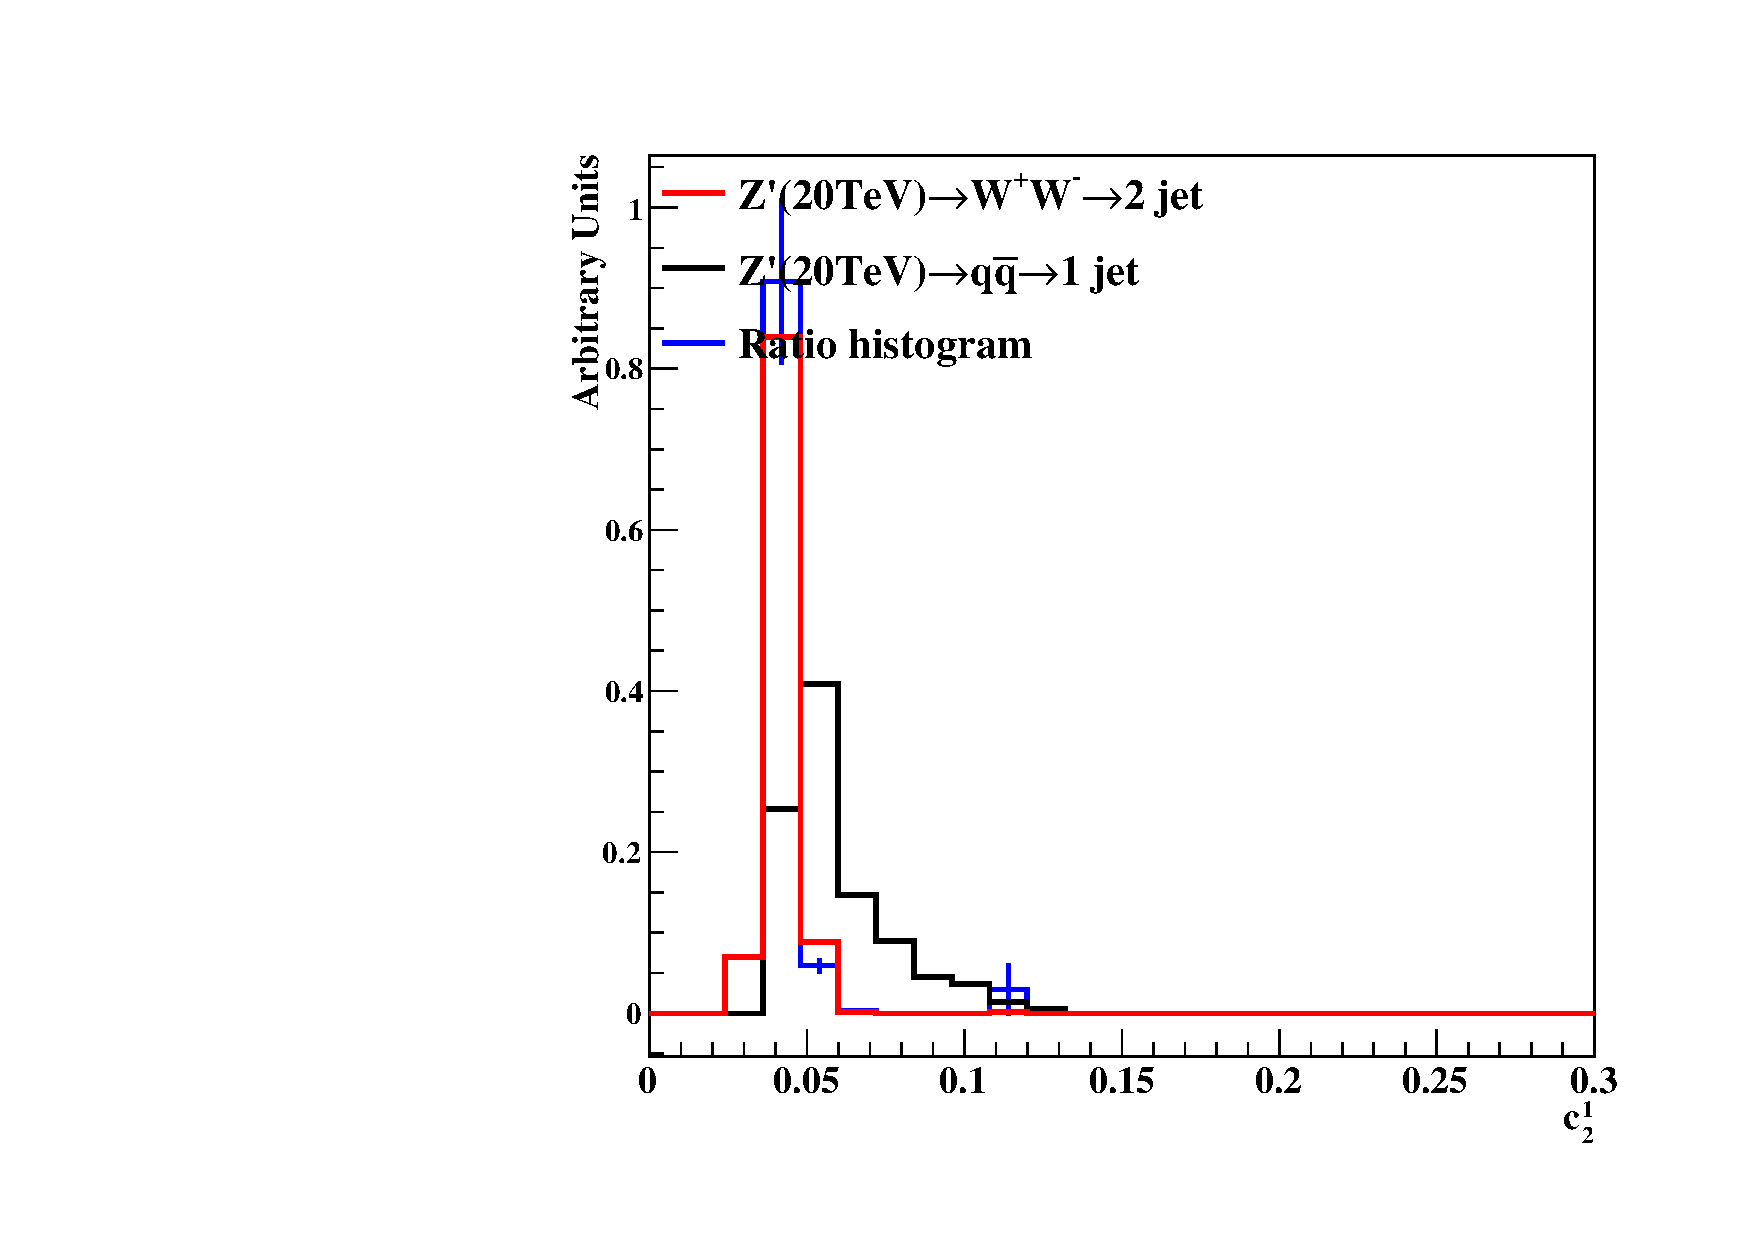
\includegraphics[width=0.22\textwidth]{figs/Rawhit_05GeV_009_c2b1_20tev_04_after_cut_25bins_Ratio.pdf}
   }
   \subfigure[40TeV at 5$\times$5(cm$\times$cm) in 0.5GeV] {
   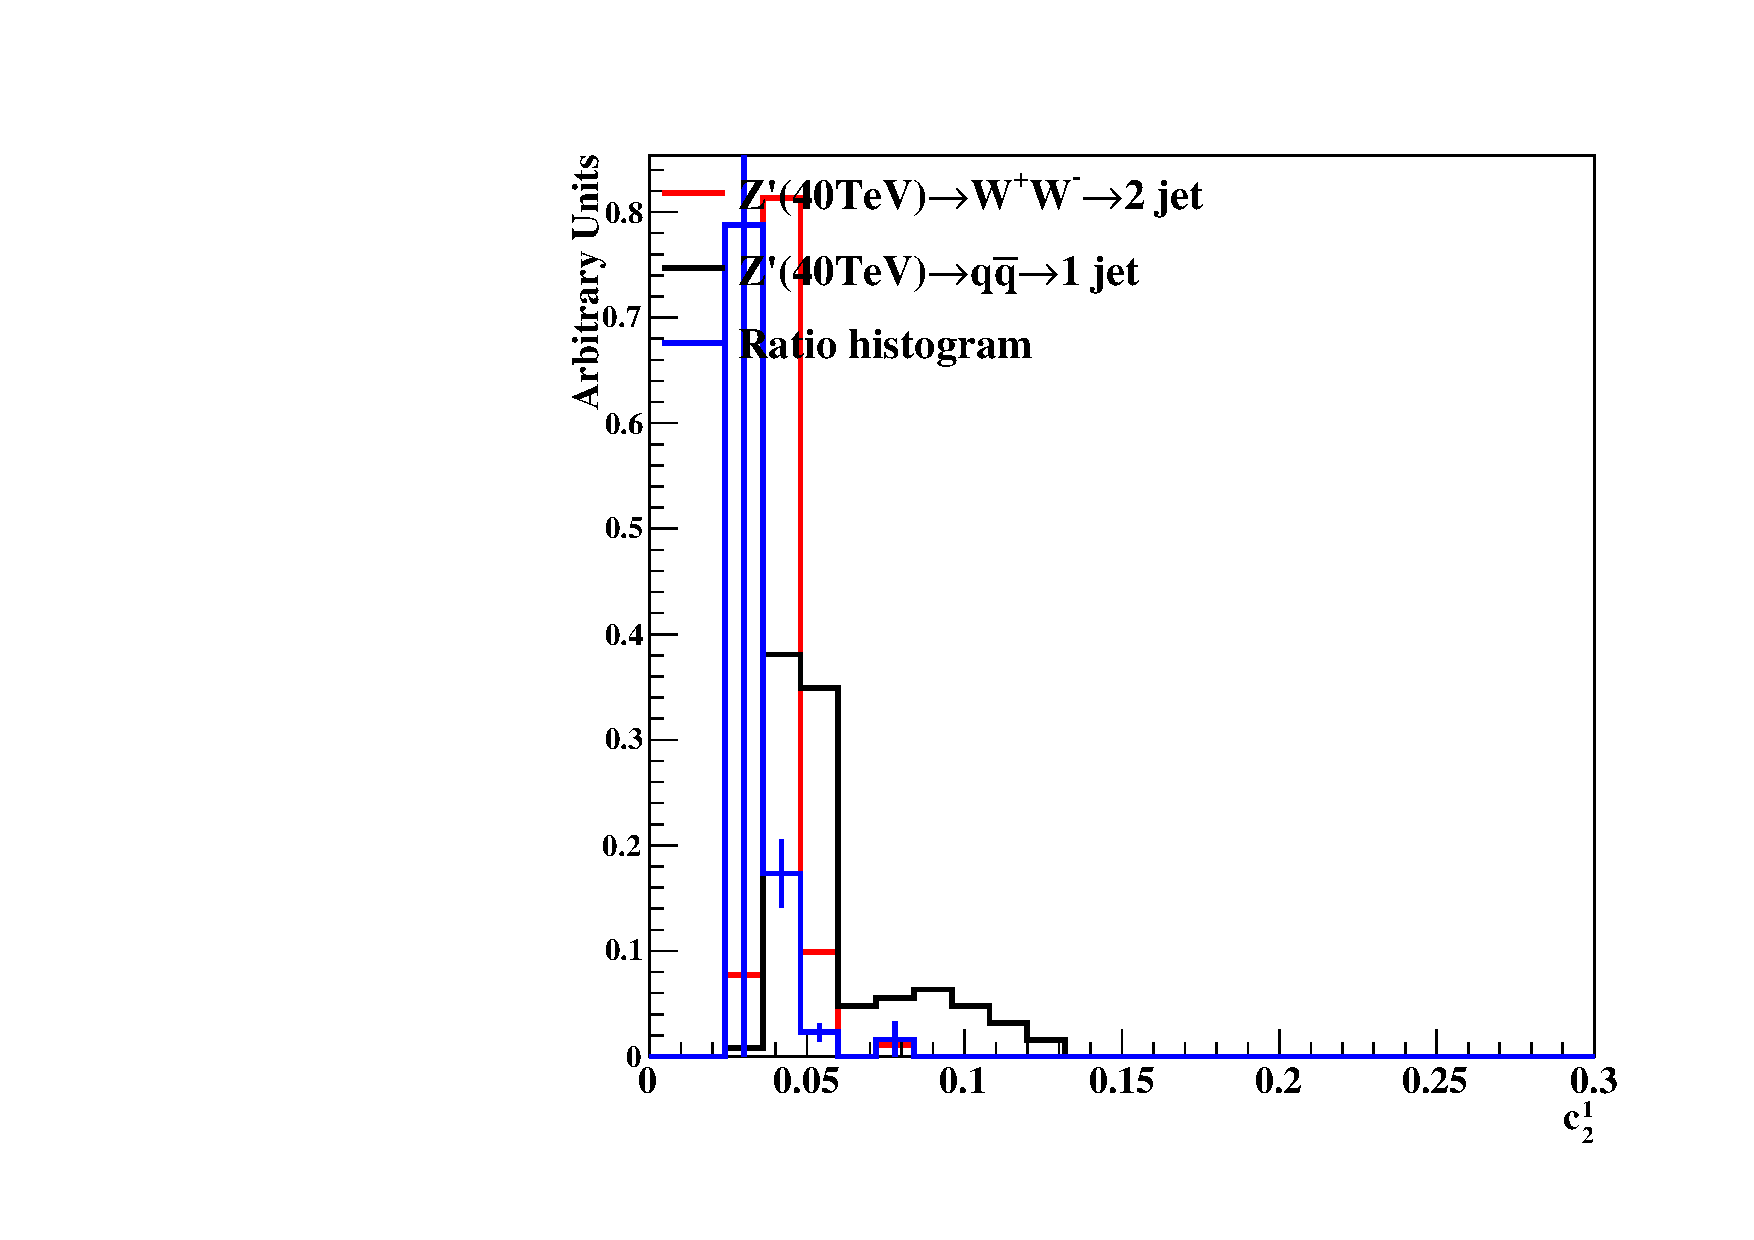
\includegraphics[width=0.22\textwidth]{figs/Rawhit_05GeV_009_c2b1_40tev_04_after_cut_25bins_Ratio.pdf}
   }
   \subfigure[5TeV at 1$\times$1(cm$\times$cm) in 0.5GeV] {
   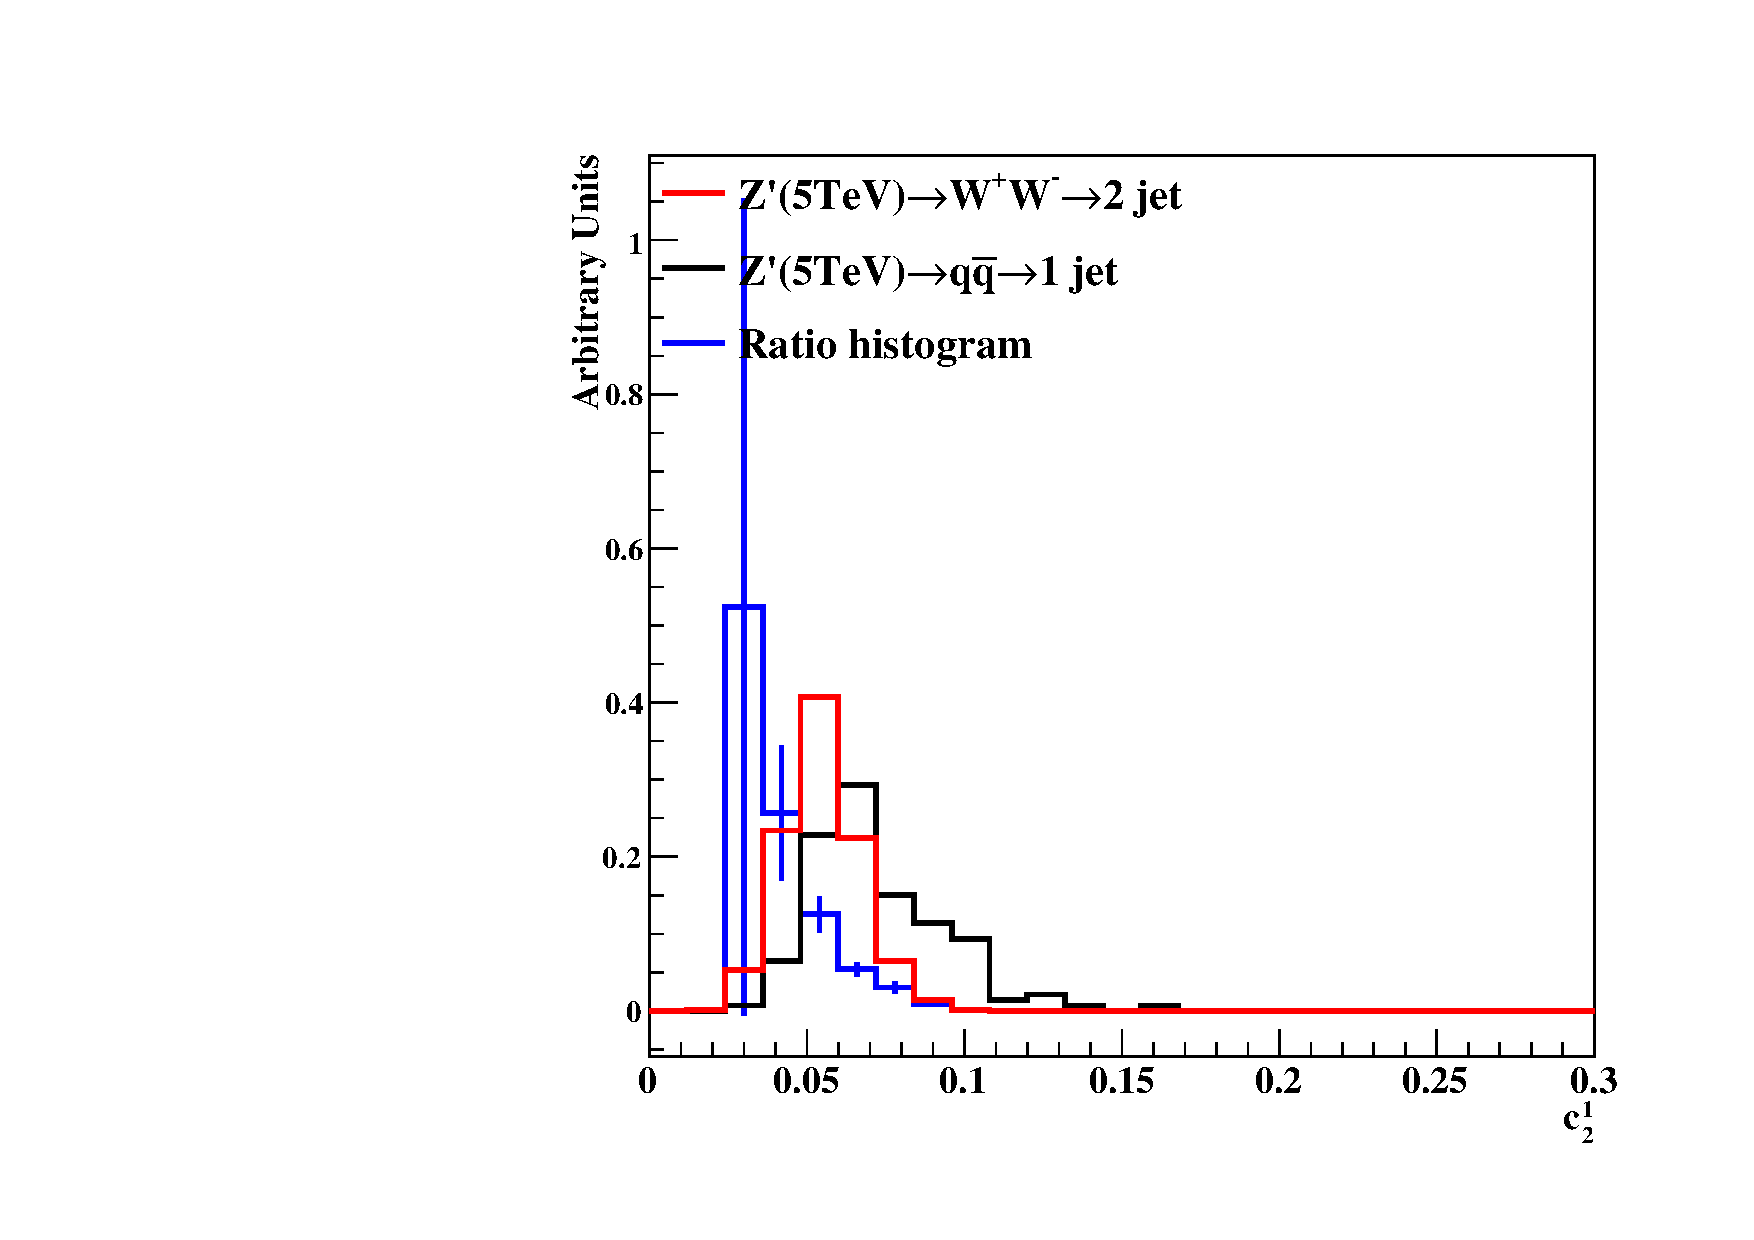
\includegraphics[width=0.22\textwidth]{figs/Rawhit_05GeV_012_c2b1_5tev_04_after_cut_25bins_Ratio.pdf}
   }
   \subfigure[10TeV at 1$\times$1(cm$\times$cm) in 0.5GeV] {
   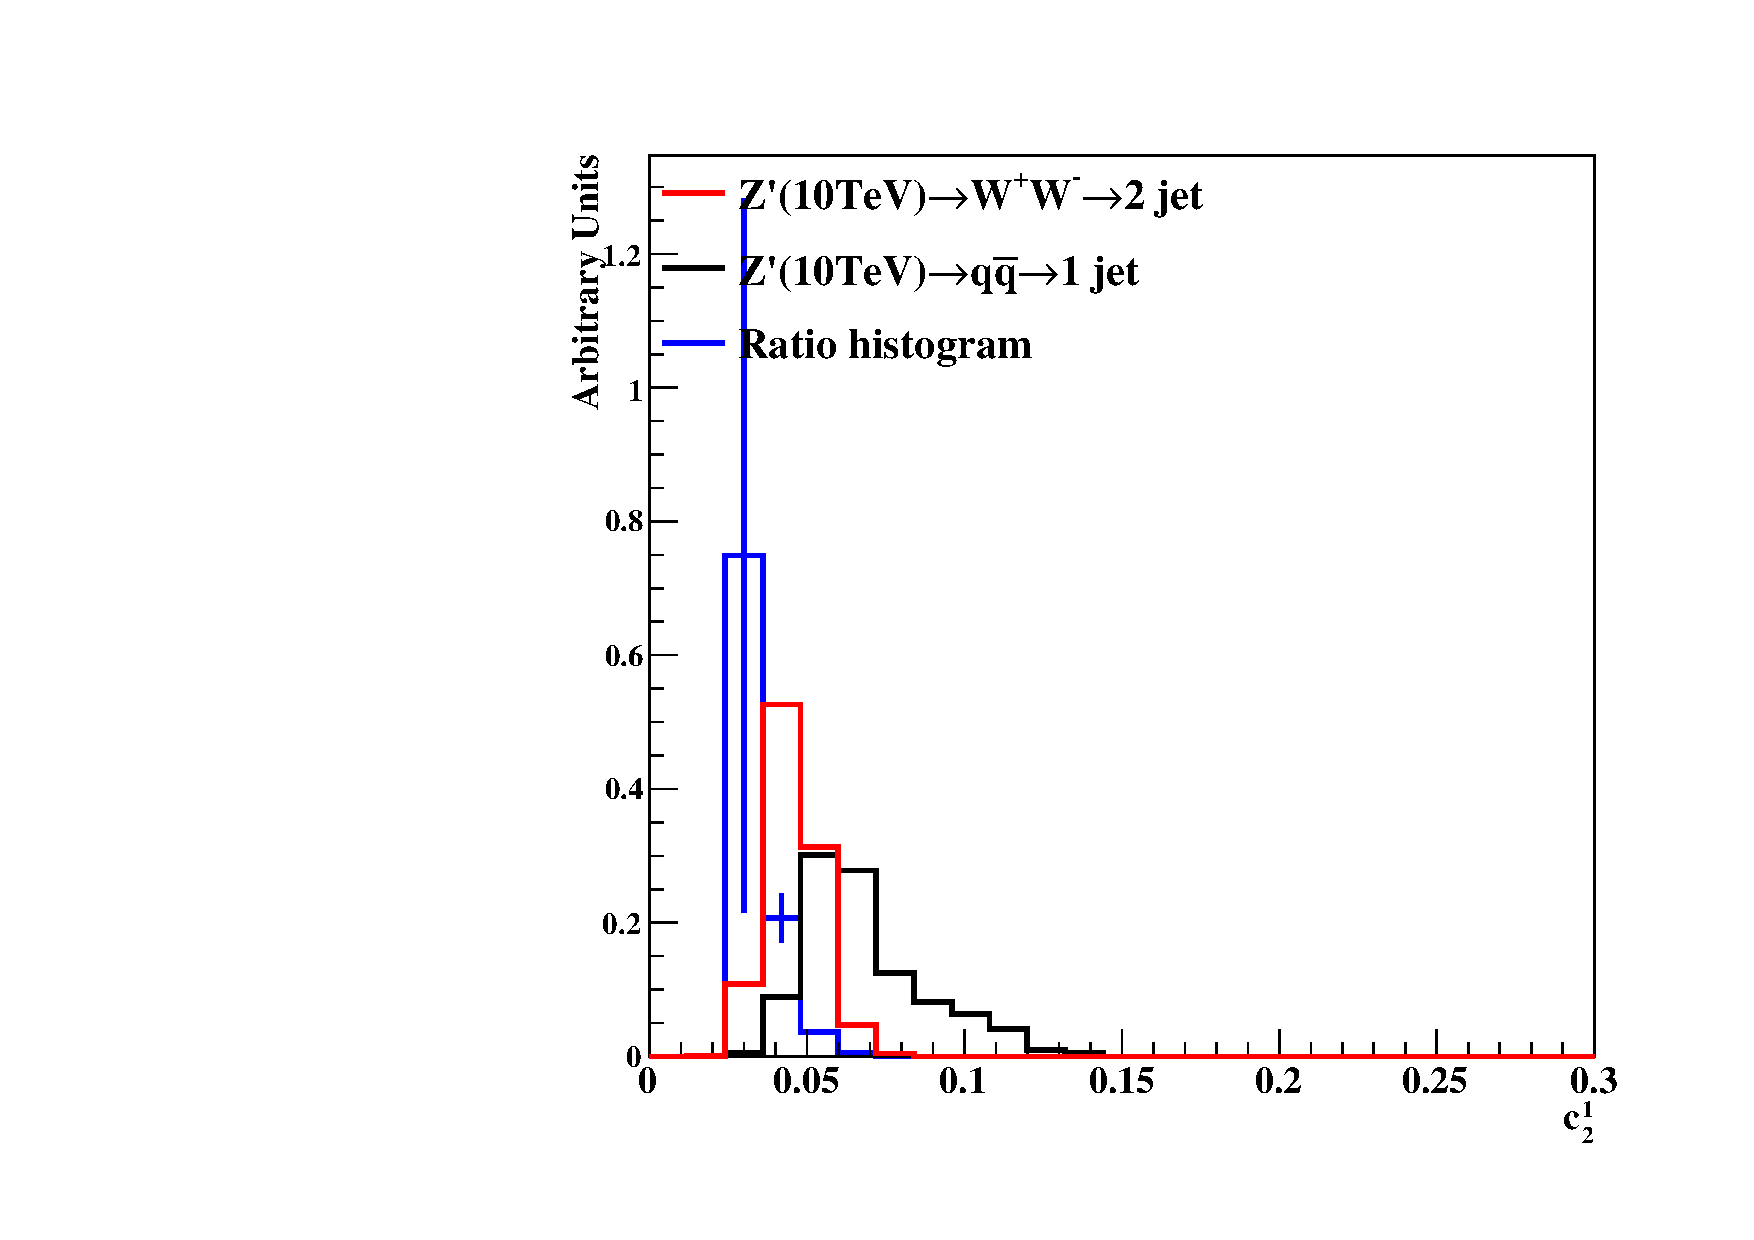
\includegraphics[width=0.22\textwidth]{figs/Rawhit_05GeV_012_c2b1_10tev_04_after_cut_25bins_Ratio.pdf}
   }
   \subfigure[20TeV at 1$\times$1(cm$\times$cm) in 0.5GeV] {
   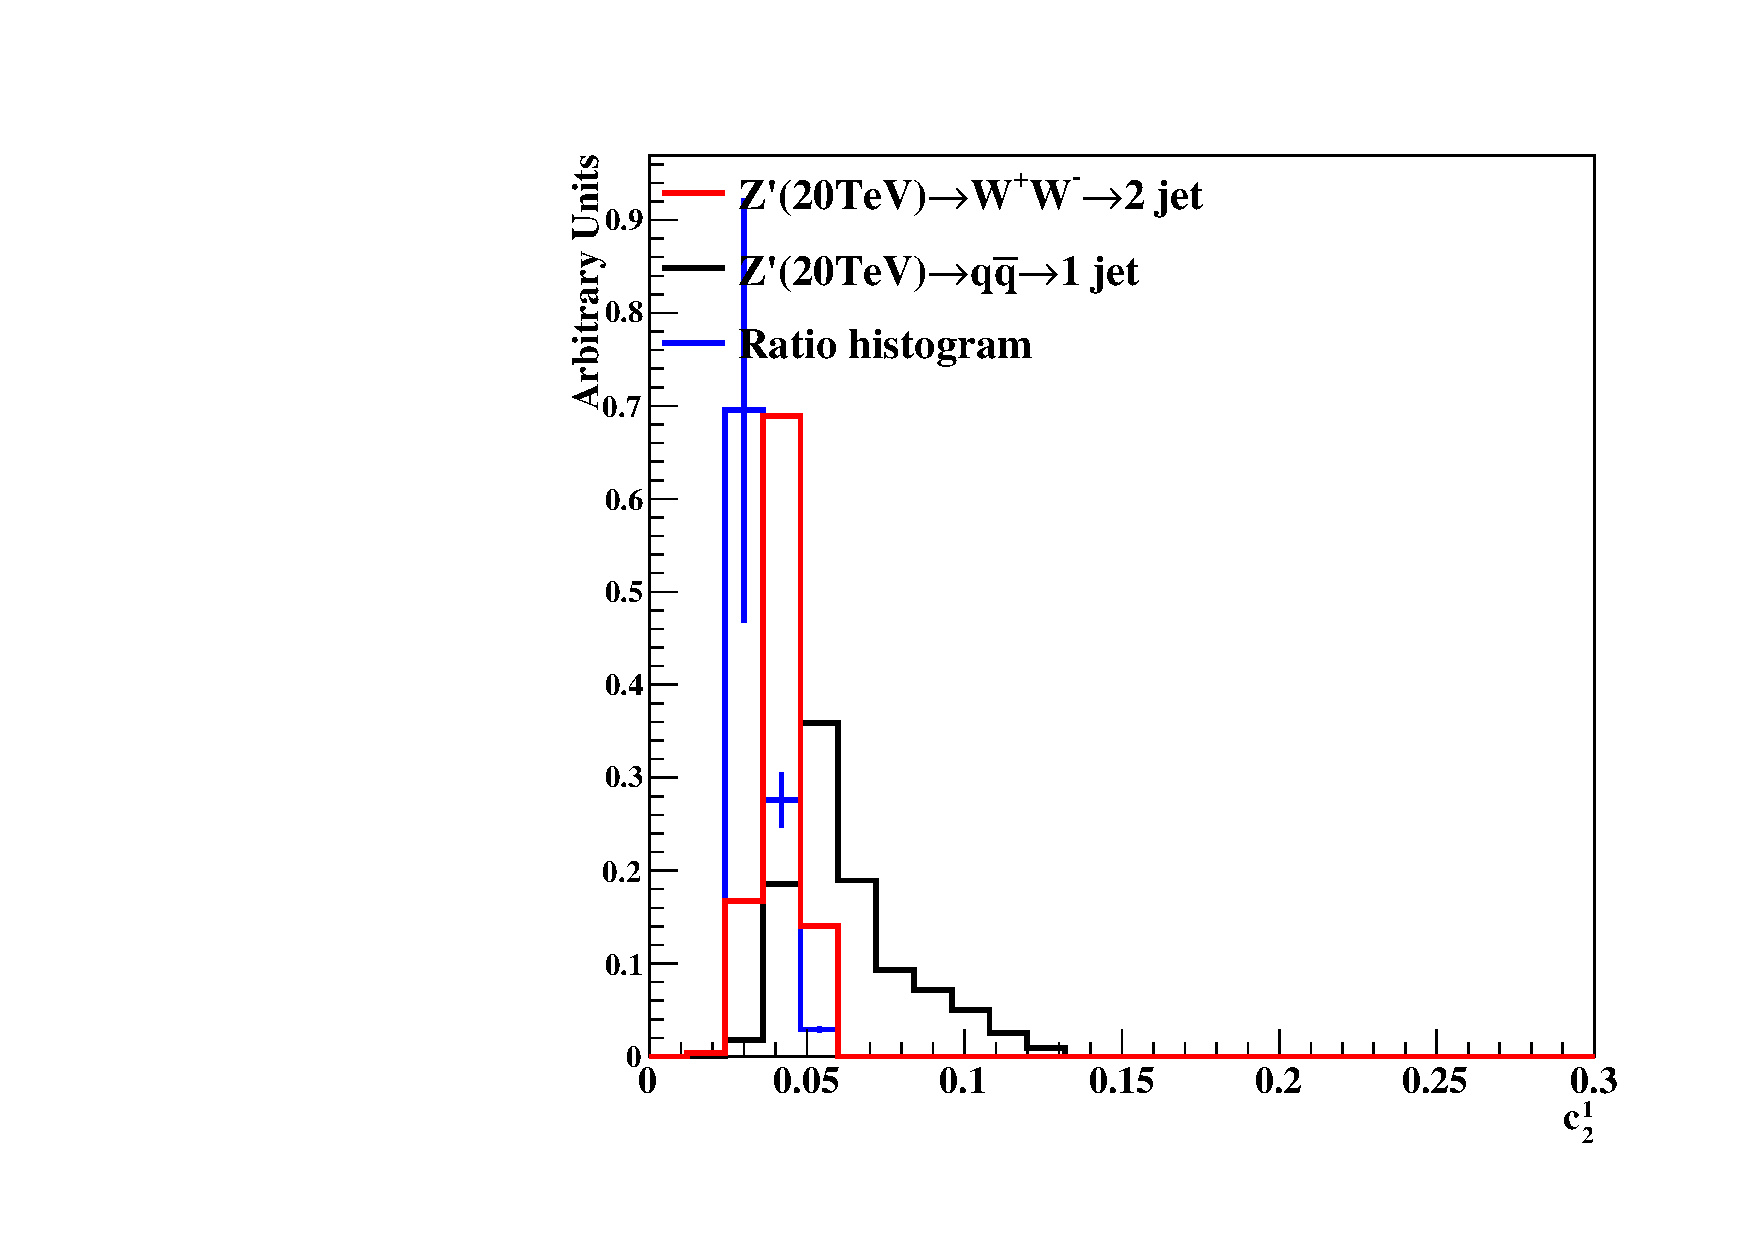
\includegraphics[width=0.22\textwidth]{figs/Rawhit_05GeV_012_c2b1_20tev_04_after_cut_25bins_Ratio.pdf}
   }
   \subfigure[40TeV at 1$\times$1(cm$\times$cm) in 0.5GeV] {
   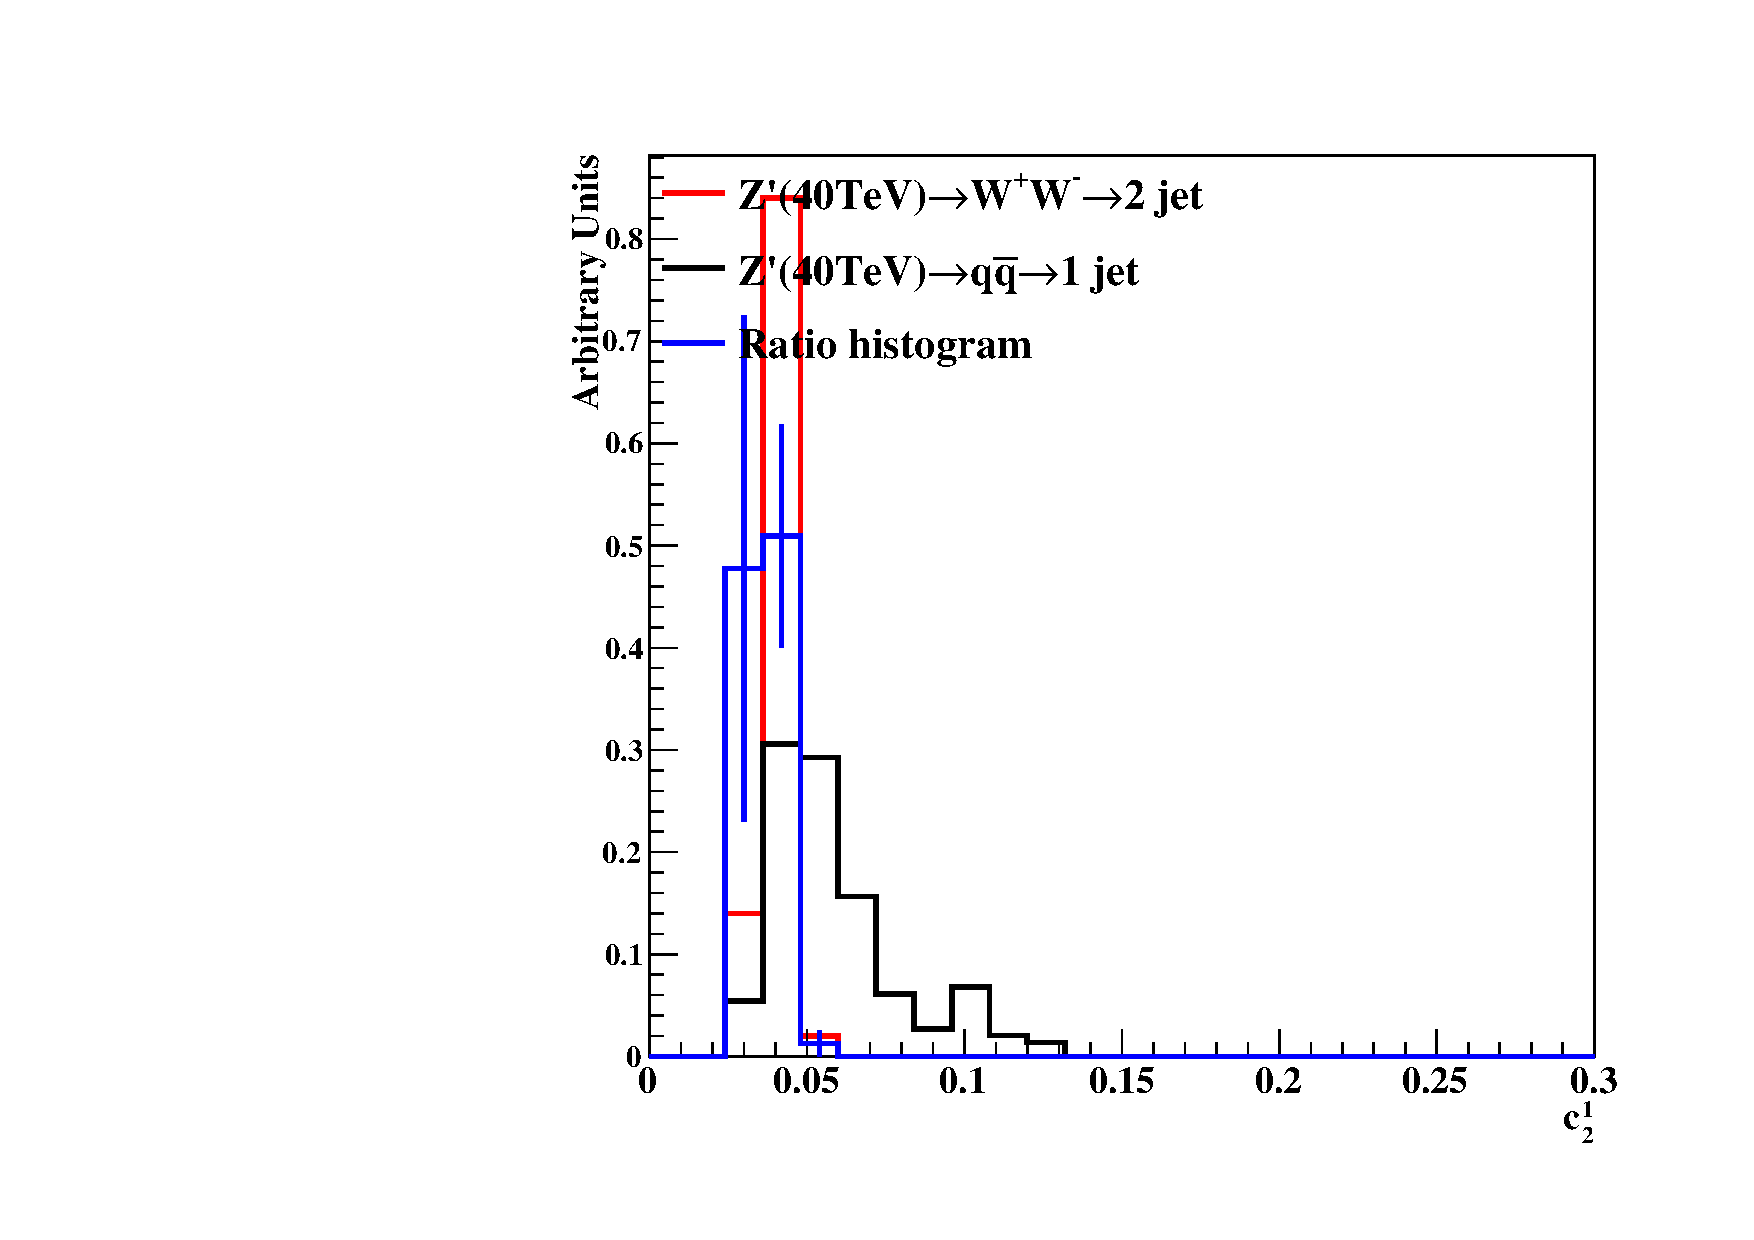
\includegraphics[width=0.22\textwidth]{figs/Rawhit_05GeV_012_c2b1_40tev_04_after_cut_25bins_Ratio.pdf}
   }\end{center}
\caption{Distributions of Mann-Whitney value U in 5, 10, 20, 40TeV energy collision for c2b1 in different detector sizes WithCut. Cell Size in 20$\times$20, 5$\times$5, and 1$\times$1(cm$\times$cm) are shown here.}
\label{fig:cluster_c2b1_tau32}
\end{figure}

\begin{figure}
\begin{center}
   \subfigure[5 TeV using Rawhit 0.5GeV cut method with New2 after cut Method] {
   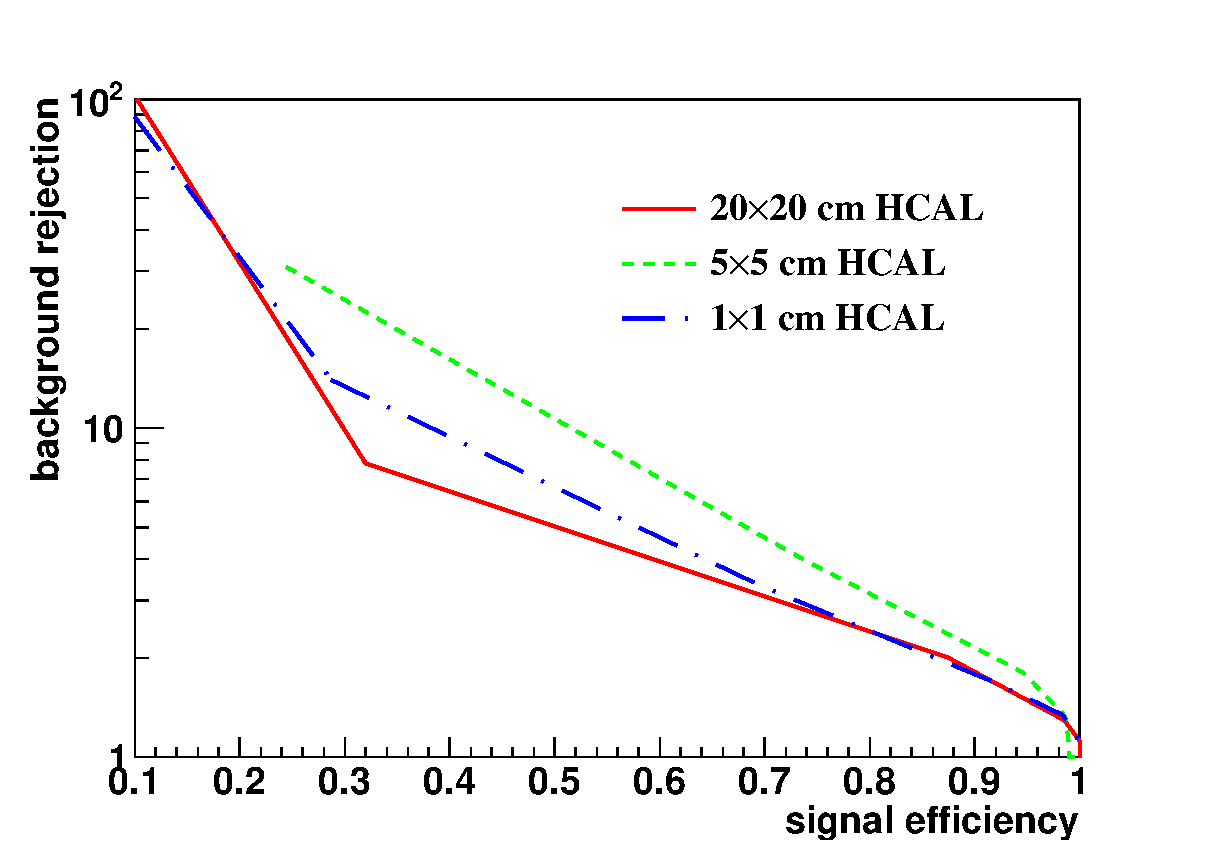
\includegraphics[width=0.43\textwidth]{figs/Rawhit_05GeV_c2b1_5tev_eff_1_New2_after_cut_25bins.eps}\hfill
   }
   \subfigure[10 TeV using Rawhit 0.5GeV cut method with New2 after cut Method] {
   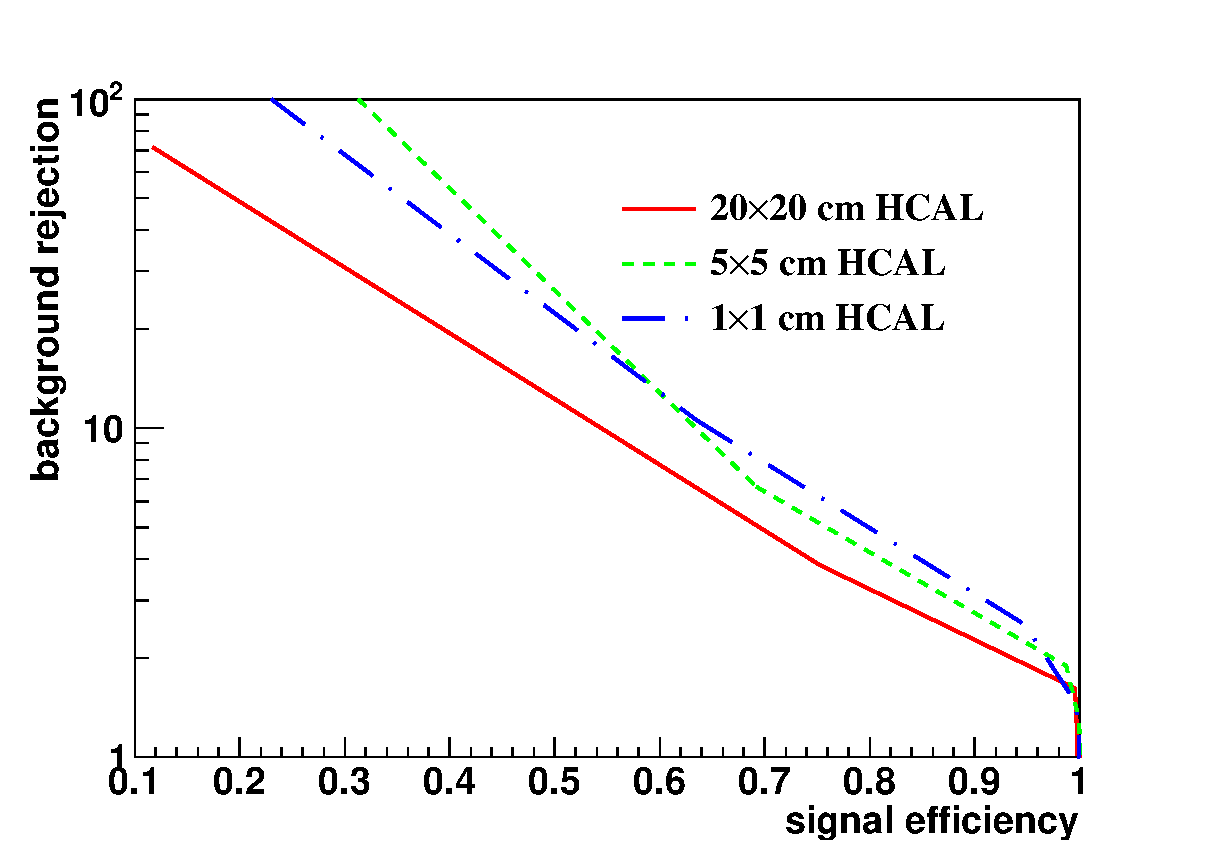
\includegraphics[width=0.43\textwidth]{figs/Rawhit_05GeV_c2b1_10tev_eff_1_New2_after_cut_25bins.eps}
   }
   \subfigure[20 TeV using Rawhit 0.5GeV cut method with New2 after cut Method] {
   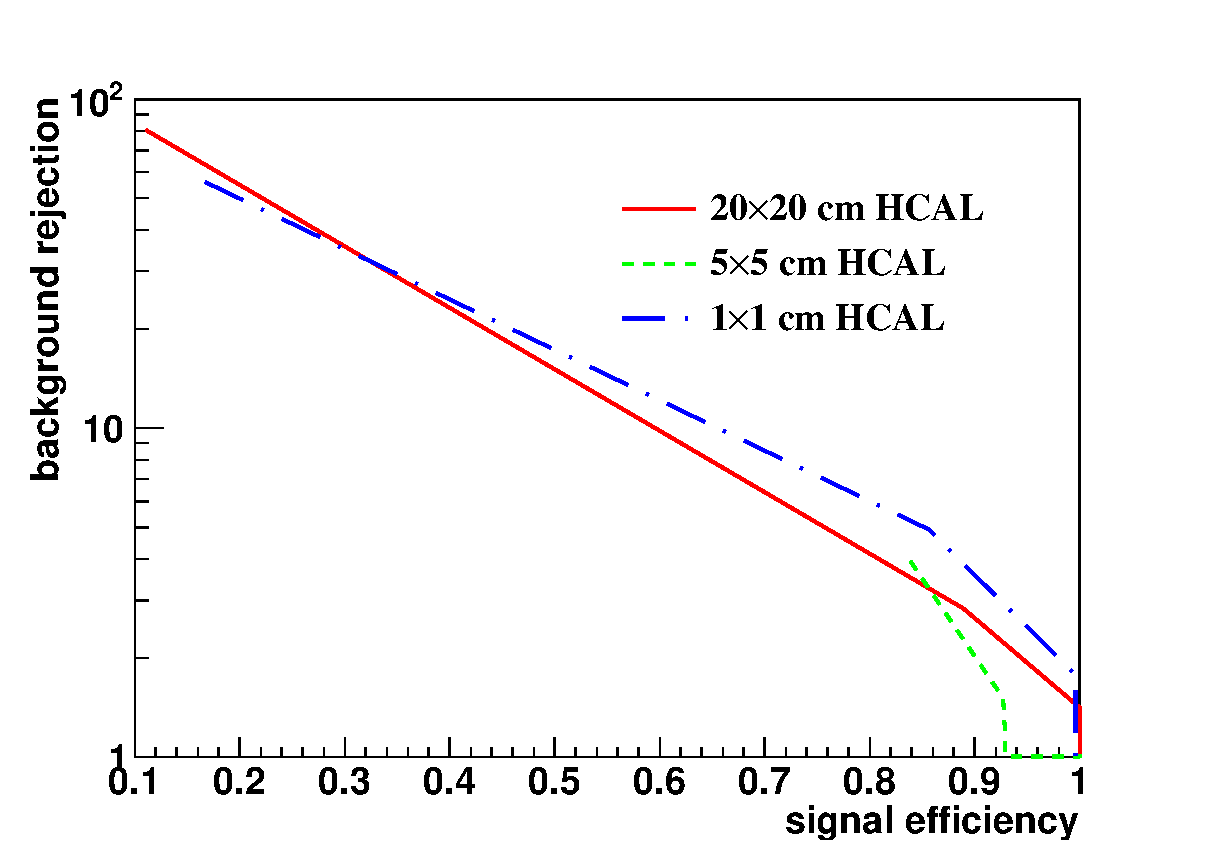
\includegraphics[width=0.43\textwidth]{figs/Rawhit_05GeV_c2b1_20tev_eff_1_New2_after_cut_25bins.eps}
   }
   \subfigure[40 TeV using Rawhit 0.5GeV cut method with New2 after cut Method] {
   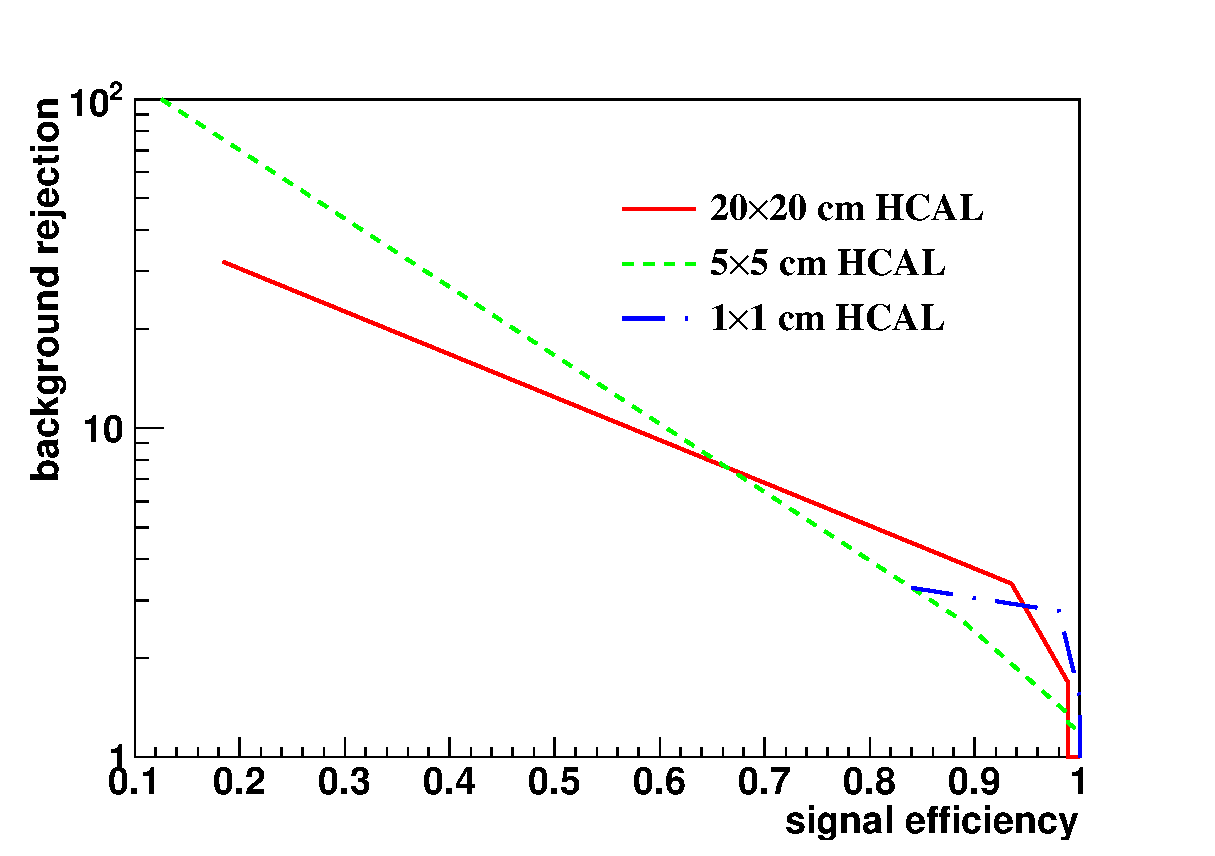
\includegraphics[width=0.43\textwidth]{figs/Rawhit_05GeV_c2b1_40tev_eff_1_New2_after_cut_25bins.eps}
   }
\end{center}
\caption{Signal efficiency versus background rejection rate using c2b1 WithCut.The energies of collision at (a)5, (b)10, (c)20, (d)40TeV are shown here. In each picture, the three ROC curves correspond to different detector sizes.}
\label{fig:cluster_c2b1}
\end{figure}

\iffalse
%25bins
\begin{figure}
\begin{center}
   \subfigure[5TeV at 20$\times$20(cm$\times$cm) in 0.25GeV] {
   \includegraphics[width=0.22\textwidth]{figs/Rawhit_025GeV_010_c2b1_5tev_04_Man.eps}\hfill
   }
   \subfigure[10TeV at 20$\times$20(cm$\times$cm) in 0.25GeV] {
   \includegraphics[width=0.22\textwidth]{figs/Rawhit_025GeV_010_c2b1_10tev_04_Man.eps}
   }
   \subfigure[20TeV at 20$\times$20(cm$\times$cm) in 0.25GeV] {
   \includegraphics[width=0.22\textwidth]{figs/Rawhit_025GeV_010_c2b1_20tev_04_Man.eps}
   }
   \subfigure[40TeV at 20$\times$20(cm$\times$cm) in 0.25GeV] {
   \includegraphics[width=0.22\textwidth]{figs/Rawhit_025GeV_010_c2b1_40tev_04_Man.eps}
   }
   \subfigure[5TeV at 5$\times$5(cm$\times$cm) in 0.25GeV] {
   \includegraphics[width=0.22\textwidth]{figs/Rawhit_025GeV_009_c2b1_5tev_04_Man.eps}
   }
   \subfigure[10TeV at 5$\times$5(cm$\times$cm) in 0.25GeV] {
   \includegraphics[width=0.22\textwidth]{figs/Rawhit_025GeV_009_c2b1_10tev_04_Man.eps}
   }
   \subfigure[20TeV at 5$\times$5(cm$\times$cm) in 0.25GeV] {
   \includegraphics[width=0.22\textwidth]{figs/Rawhit_025GeV_009_c2b1_20tev_04_Man.eps}
   }
   \subfigure[40TeV at 5$\times$5(cm$\times$cm) in 0.25GeV] {
   \includegraphics[width=0.22\textwidth]{figs/Rawhit_025GeV_009_c2b1_40tev_04_Man.eps}
   }
   \subfigure[5TeV at 1$\times$1(cm$\times$cm) in 0.25GeV] {
   \includegraphics[width=0.22\textwidth]{figs/Rawhit_025GeV_012_c2b1_5tev_04_Man.eps}
   }
   \subfigure[10TeV at 1$\times$1(cm$\times$cm) in 0.25GeV] {
   \includegraphics[width=0.22\textwidth]{figs/Rawhit_025GeV_012_c2b1_10tev_04_Man.eps}
   }
   \subfigure[20TeV at 1$\times$1(cm$\times$cm) in 0.25GeV] {
   \includegraphics[width=0.22\textwidth]{figs/Rawhit_025GeV_012_c2b1_20tev_04_Man.eps}
   }
   \subfigure[40TeV at 1$\times$1(cm$\times$cm) in 0.25GeV] {
   \includegraphics[width=0.22\textwidth]{figs/Rawhit_025GeV_012_c2b1_40tev_04_Man.eps}
   }\end{center}
\caption{Distributions of Mann-Whitney value U in 5, 10, 20, 40TeV energy collision for c2b1 in different detector sizes. Cell Size in 20$\times$20, 5$\times$5, and 1$\times$1(cm$\times$cm) are shown here.}
\label{fig:cluster_c2b1_tau32}
\end{figure}

\begin{figure}
\begin{center}
   \subfigure[5 TeV using Rawhit 0.25GeV cut method with New2 after cut Method] {
   \includegraphics[width=0.43\textwidth]{figs/Rawhit_025GeV_c2b1_5tev_eff_1_New2_no_cut_25bins.eps}\hfill
   }
   \subfigure[10 TeV using Rawhit 0.25GeV cut method with New2 after cut Method] {
   \includegraphics[width=0.43\textwidth]{figs/Rawhit_025GeV_c2b1_10tev_eff_1_New2_no_cut_25bins.eps}
   }
   \subfigure[20 TeV using Rawhit 0.25GeV cut method with New2 after cut Method] {
   \includegraphics[width=0.43\textwidth]{figs/Rawhit_025GeV_c2b1_20tev_eff_1_New2_no_cut_25bins.eps}
   }
   \subfigure[40 TeV using Rawhit 0.25GeV cut method with New2 after cut Method] {
   \includegraphics[width=0.43\textwidth]{figs/Rawhit_025GeV_c2b1_40tev_eff_1_New2_no_cut_25bins.eps}
   }
\end{center}
\caption{Signal efficiency versus background rejection rate using c2b1The energies of collision at (a)5, (b)10, (c)20, (d)40TeV are shown here. In each picture, the three ROC curves correspond to different detector sizes.}
\label{fig:cluster_c2b1}
\end{figure}
\fi

\iffalse
%25bins
\begin{figure}
\begin{center}
   \subfigure[5TeV at 20$\times$20(cm$\times$cm) in cluster] {
   \includegraphics[width=0.22\textwidth]{figs/Dis_cluster_010_tau21_5tev_04_Man.eps}\hfill
   }
   \subfigure[10TeV at 20$\times$20(cm$\times$cm) in cluster] {
   \includegraphics[width=0.22\textwidth]{figs/Dis_cluster_010_tau21_10tev_04_Man.eps}
   }
   \subfigure[20TeV at 20$\times$20(cm$\times$cm) in cluster] {
   \includegraphics[width=0.22\textwidth]{figs/Dis_cluster_010_tau21_20tev_04_Man.eps}
   }
   \subfigure[40TeV at 20$\times$20(cm$\times$cm) in cluster] {
   \includegraphics[width=0.22\textwidth]{figs/Dis_cluster_010_tau21_40tev_04_Man.eps}
   }
   \subfigure[5TeV at 5$\times$5(cm$\times$cm) in cluster] {
   \includegraphics[width=0.22\textwidth]{figs/Dis_cluster_009_tau21_5tev_04_Man.eps}
   }
   \subfigure[10TeV at 5$\times$5(cm$\times$cm) in cluster] {
   \includegraphics[width=0.22\textwidth]{figs/Dis_cluster_009_tau21_10tev_04_Man.eps}
   }
   \subfigure[20TeV at 5$\times$5(cm$\times$cm) in cluster] {
   \includegraphics[width=0.22\textwidth]{figs/Dis_cluster_009_tau21_20tev_04_Man.eps}
   }
   \subfigure[40TeV at 5$\times$5(cm$\times$cm) in cluster] {
   \includegraphics[width=0.22\textwidth]{figs/Dis_cluster_009_tau21_40tev_04_Man.eps}
   }
   \subfigure[5TeV at 1$\times$1(cm$\times$cm) in cluster] {
   \includegraphics[width=0.22\textwidth]{figs/Dis_cluster_012_tau21_5tev_04_Man.eps}
   }
   \subfigure[10TeV at 1$\times$1(cm$\times$cm) in cluster] {
   \includegraphics[width=0.22\textwidth]{figs/Dis_cluster_012_tau21_10tev_04_Man.eps}
   }
   \subfigure[20TeV at 1$\times$1(cm$\times$cm) in cluster] {
   \includegraphics[width=0.22\textwidth]{figs/Dis_cluster_012_tau21_20tev_04_Man.eps}
   }
   \subfigure[40TeV at 1$\times$1(cm$\times$cm) in cluster] {
   \includegraphics[width=0.22\textwidth]{figs/Dis_cluster_012_tau21_40tev_04_Man.eps}
   }
\end{center}
\caption{Distributions of Mann-Whitney value U in 5,10,20,40TeV energy collision for $\tau_{21}$  in different detector sizes. Cell Size in 20$\times$20, 5$\times$5, and 1$\times$1(cm$\times$cm) are shown here.}
\label{fig:cluster_tau21_tau32}
\end{figure}

\begin{figure}
\begin{center}
   \subfigure[5 TeV using cluster method with New2 after cut Method] {
   \includegraphics[width=0.43\textwidth]{figs/cluster_tau21_5tev_eff_1_New2_no_cut_25bins.eps}\hfill
   }
   \subfigure[10 TeV using cluster method with New2 after cut Method] {
   \includegraphics[width=0.43\textwidth]{figs/cluster_tau21_10tev_eff_1_New2_no_cut_25bins.eps}
   }
   \subfigure[20 TeV using cluster method with New2 after cut Method] {
   \includegraphics[width=0.43\textwidth]{figs/cluster_tau21_20tev_eff_1_New2_no_cut_25bins.eps}
   }
   \subfigure[40 TeV using cluster method with New2 after cut Method] {
   \includegraphics[width=0.43\textwidth]{figs/cluster_tau21_40tev_eff_1_New2_no_cut_25bins.eps}
   }
\end{center}
\caption{Signal efficiency versus background rejection rate using $\tau_{21}$.The energies of collision at (a)5, (b)10, (c)20, (d)40TeV are shown here. In each picture, the three ROC curves correspond to different detector sizes.}
\label{fig:cluster_tau21}
\end{figure}
\fi

%25bins
\begin{figure}
\begin{center}
   \subfigure[5TeV at 20$\times$20(cm$\times$cm) in 0.5GeV] {
   \includegraphics[width=0.22\textwidth]{figs/Rawhit_05GeV_010_tau21_5tev_04_no_cut_25bins_Ratio.pdf}\hfill
   }
   \subfigure[10TeV at 20$\times$20(cm$\times$cm) in 0.5GeV] {
   \includegraphics[width=0.22\textwidth]{figs/Rawhit_05GeV_010_tau21_10tev_04_no_cut_25bins_Ratio.pdf}
   }
   \subfigure[20TeV at 20$\times$20(cm$\times$cm) in 0.5GeV] {
   \includegraphics[width=0.22\textwidth]{figs/Rawhit_05GeV_010_tau21_20tev_04_no_cut_25bins_Ratio.pdf}
   }
   \subfigure[40TeV at 20$\times$20(cm$\times$cm) in 0.5GeV] {
   \includegraphics[width=0.22\textwidth]{figs/Rawhit_05GeV_010_tau21_40tev_04_no_cut_25bins_Ratio.pdf}
   }
   \subfigure[5TeV at 5$\times$5(cm$\times$cm) in 0.5GeV] {
   \includegraphics[width=0.22\textwidth]{figs/Rawhit_05GeV_009_tau21_5tev_04_no_cut_25bins_Ratio.pdf}
   }
   \subfigure[10TeV at 5$\times$5(cm$\times$cm) in 0.5GeV] {
   \includegraphics[width=0.22\textwidth]{figs/Rawhit_05GeV_009_tau21_10tev_04_no_cut_25bins_Ratio.pdf}
   }
   \subfigure[20TeV at 5$\times$5(cm$\times$cm) in 0.5GeV] {
   \includegraphics[width=0.22\textwidth]{figs/Rawhit_05GeV_009_tau21_20tev_04_no_cut_25bins_Ratio.pdf}
   }
   \subfigure[40TeV at 5$\times$5(cm$\times$cm) in 0.5GeV] {
   \includegraphics[width=0.22\textwidth]{figs/Rawhit_05GeV_009_tau21_40tev_04_no_cut_25bins_Ratio.pdf}
   }
   \subfigure[5TeV at 1$\times$1(cm$\times$cm) in 0.5GeV] {
   \includegraphics[width=0.22\textwidth]{figs/Rawhit_05GeV_012_tau21_5tev_04_no_cut_25bins_Ratio.pdf}
   }
   \subfigure[10TeV at 1$\times$1(cm$\times$cm) in 0.5GeV] {
   \includegraphics[width=0.22\textwidth]{figs/Rawhit_05GeV_012_tau21_10tev_04_no_cut_25bins_Ratio.pdf}
   }
   \subfigure[20TeV at 1$\times$1(cm$\times$cm) in 0.5GeV] {
   \includegraphics[width=0.22\textwidth]{figs/Rawhit_05GeV_012_tau21_20tev_04_no_cut_25bins_Ratio.pdf}
   }
   \subfigure[40TeV at 1$\times$1(cm$\times$cm) in 0.5GeV] {
   \includegraphics[width=0.22\textwidth]{figs/Rawhit_05GeV_012_tau21_40tev_04_no_cut_25bins_Ratio.pdf}
   }\end{center}
\caption{Distributions of Mann-Whitney value U in 5, 10, 20, 40TeV energy collision for $\tau_{21}$  in different detector sizes WithoutCut. Cell Size in 20$\times$20, 5$\times$5, and 1$\times$1(cm$\times$cm) are shown here.}
\label{fig:cluster_tau21_tau32}
\end{figure}

\begin{figure}
\begin{center}
   \subfigure[5 TeV using Rawhit 0.5GeV cut method with New2 no cut Method] {
   \includegraphics[width=0.43\textwidth]{figs/Rawhit_05GeV_tau21_5tev_eff_1_New2_no_cut_25bins.eps}\hfill
   }
   \subfigure[10 TeV using Rawhit 0.5GeV cut method with New2 no cut Method] {
   \includegraphics[width=0.43\textwidth]{figs/Rawhit_05GeV_tau21_10tev_eff_1_New2_no_cut_25bins.eps}
   }
   \subfigure[20 TeV using Rawhit 0.5GeV cut method with New2 no cut Method] {
   \includegraphics[width=0.43\textwidth]{figs/Rawhit_05GeV_tau21_20tev_eff_1_New2_no_cut_25bins.eps}
   }
   \subfigure[40 TeV using Rawhit 0.5GeV cut method with New2 no cut Method] {
   \includegraphics[width=0.43\textwidth]{figs/Rawhit_05GeV_tau21_40tev_eff_1_New2_no_cut_25bins.eps}
   }
\end{center}
\caption{Signal efficiency versus background rejection rate using $\tau_{21}$ WithoutCut.The energies of collision at (a)5, (b)10, (c)20, (d)40TeV are shown here. In each picture, the three ROC curves correspond to different detector sizes.}
\label{fig:cluster_tau21}
\end{figure}

%25bins
\begin{figure}
\begin{center}
   \subfigure[5TeV at 20$\times$20(cm$\times$cm) in 0.5GeV] {
   \includegraphics[width=0.22\textwidth]{figs/Rawhit_05GeV_010_tau21_5tev_04_after_cut_25bins_Ratio.pdf}\hfill
   }
   \subfigure[10TeV at 20$\times$20(cm$\times$cm) in 0.5GeV] {
   \includegraphics[width=0.22\textwidth]{figs/Rawhit_05GeV_010_tau21_10tev_04_after_cut_25bins_Ratio.pdf}
   }
   \subfigure[20TeV at 20$\times$20(cm$\times$cm) in 0.5GeV] {
   \includegraphics[width=0.22\textwidth]{figs/Rawhit_05GeV_010_tau21_20tev_04_after_cut_25bins_Ratio.pdf}
   }
   \subfigure[40TeV at 20$\times$20(cm$\times$cm) in 0.5GeV] {
   \includegraphics[width=0.22\textwidth]{figs/Rawhit_05GeV_010_tau21_40tev_04_after_cut_25bins_Ratio.pdf}
   }
   \subfigure[5TeV at 5$\times$5(cm$\times$cm) in 0.5GeV] {
   \includegraphics[width=0.22\textwidth]{figs/Rawhit_05GeV_009_tau21_5tev_04_after_cut_25bins_Ratio.pdf}
   }
   \subfigure[10TeV at 5$\times$5(cm$\times$cm) in 0.5GeV] {
   \includegraphics[width=0.22\textwidth]{figs/Rawhit_05GeV_009_tau21_10tev_04_after_cut_25bins_Ratio.pdf}
   }
   \subfigure[20TeV at 5$\times$5(cm$\times$cm) in 0.5GeV] {
   \includegraphics[width=0.22\textwidth]{figs/Rawhit_05GeV_009_tau21_20tev_04_after_cut_25bins_Ratio.pdf}
   }
   \subfigure[40TeV at 5$\times$5(cm$\times$cm) in 0.5GeV] {
   \includegraphics[width=0.22\textwidth]{figs/Rawhit_05GeV_009_tau21_40tev_04_after_cut_25bins_Ratio.pdf}
   }
   \subfigure[5TeV at 1$\times$1(cm$\times$cm) in 0.5GeV] {
   \includegraphics[width=0.22\textwidth]{figs/Rawhit_05GeV_012_tau21_5tev_04_after_cut_25bins_Ratio.pdf}
   }
   \subfigure[10TeV at 1$\times$1(cm$\times$cm) in 0.5GeV] {
   \includegraphics[width=0.22\textwidth]{figs/Rawhit_05GeV_012_tau21_10tev_04_after_cut_25bins_Ratio.pdf}
   }
   \subfigure[20TeV at 1$\times$1(cm$\times$cm) in 0.5GeV] {
   \includegraphics[width=0.22\textwidth]{figs/Rawhit_05GeV_012_tau21_20tev_04_after_cut_25bins_Ratio.pdf}
   }
   \subfigure[40TeV at 1$\times$1(cm$\times$cm) in 0.5GeV] {
   \includegraphics[width=0.22\textwidth]{figs/Rawhit_05GeV_012_tau21_40tev_04_after_cut_25bins_Ratio.pdf}
   }\end{center}
\caption{Distributions of Mann-Whitney value U in 5, 10, 20, 40TeV energy collision for $\tau_{21}$  in different detector sizes WithCut. Cell Size in 20$\times$20, 5$\times$5, and 1$\times$1(cm$\times$cm) are shown here.}
\label{fig:cluster_tau21_tau32}
\end{figure}
\begin{figure}
\begin{center}
   \subfigure[5 TeV using Rawhit 0.5GeV cut method with New2 after cut Method] {
   \includegraphics[width=0.43\textwidth]{figs/Rawhit_05GeV_tau21_5tev_eff_1_New2_after_cut_25bins.eps}\hfill
   }
   \subfigure[10 TeV using Rawhit 0.5GeV cut method with New2 after cut Method] {
   \includegraphics[width=0.43\textwidth]{figs/Rawhit_05GeV_tau21_10tev_eff_1_New2_after_cut_25bins.eps}
   }
   \subfigure[20 TeV using Rawhit 0.5GeV cut method with New2 after cut Method] {
   \includegraphics[width=0.43\textwidth]{figs/Rawhit_05GeV_tau21_20tev_eff_1_New2_after_cut_25bins.eps}
   }
   \subfigure[40 TeV using Rawhit 0.5GeV cut method with New2 after cut Method] {
   \includegraphics[width=0.43\textwidth]{figs/Rawhit_05GeV_tau21_40tev_eff_1_New2_after_cut_25bins.eps}
   }
\end{center}
\caption{Signal efficiency versus background rejection rate using $\tau_{21}$ WithCut.The energies of collision at (a)5, (b)10, (c)20, (d)40TeV are shown here. In each picture, the three ROC curves correspond to different detector sizes.}
\label{fig:cluster_tau21}
\end{figure}

\iffalse
%25bins
\begin{figure}
\begin{center}
   \subfigure[5TeV at 20$\times$20(cm$\times$cm) in 0.25GeV] {
   \includegraphics[width=0.22\textwidth]{figs/Rawhit_025GeV_010_tau21_5tev_04_Man.eps}\hfill
   }
   \subfigure[10TeV at 20$\times$20(cm$\times$cm) in 0.25GeV] {
   \includegraphics[width=0.22\textwidth]{figs/Rawhit_025GeV_010_tau21_10tev_04_Man.eps}
   }
   \subfigure[20TeV at 20$\times$20(cm$\times$cm) in 0.25GeV] {
   \includegraphics[width=0.22\textwidth]{figs/Rawhit_025GeV_010_tau21_20tev_04_Man.eps}
   }
   \subfigure[40TeV at 20$\times$20(cm$\times$cm) in 0.25GeV] {
   \includegraphics[width=0.22\textwidth]{figs/Rawhit_025GeV_010_tau21_40tev_04_Man.eps}
   }
   \subfigure[5TeV at 5$\times$5(cm$\times$cm) in 0.25GeV] {
   \includegraphics[width=0.22\textwidth]{figs/Rawhit_025GeV_009_tau21_5tev_04_Man.eps}
   }
   \subfigure[10TeV at 5$\times$5(cm$\times$cm) in 0.25GeV] {
   \includegraphics[width=0.22\textwidth]{figs/Rawhit_025GeV_009_tau21_10tev_04_Man.eps}
   }
   \subfigure[20TeV at 5$\times$5(cm$\times$cm) in 0.25GeV] {
   \includegraphics[width=0.22\textwidth]{figs/Rawhit_025GeV_009_tau21_20tev_04_Man.eps}
   }
   \subfigure[40TeV at 5$\times$5(cm$\times$cm) in 0.25GeV] {
   \includegraphics[width=0.22\textwidth]{figs/Rawhit_025GeV_009_tau21_40tev_04_Man.eps}
   }
   \subfigure[5TeV at 1$\times$1(cm$\times$cm) in 0.25GeV] {
   \includegraphics[width=0.22\textwidth]{figs/Rawhit_025GeV_012_tau21_5tev_04_Man.eps}
   }
   \subfigure[10TeV at 1$\times$1(cm$\times$cm) in 0.25GeV] {
   \includegraphics[width=0.22\textwidth]{figs/Rawhit_025GeV_012_tau21_10tev_04_Man.eps}
   }
   \subfigure[20TeV at 1$\times$1(cm$\times$cm) in 0.25GeV] {
   \includegraphics[width=0.22\textwidth]{figs/Rawhit_025GeV_012_tau21_20tev_04_Man.eps}
   }
   \subfigure[40TeV at 1$\times$1(cm$\times$cm) in 0.25GeV] {
   \includegraphics[width=0.22\textwidth]{figs/Rawhit_025GeV_012_tau21_40tev_04_Man.eps}
   }\end{center}
\caption{Distributions of Mann-Whitney value U in 5, 10, 20, 40TeV energy collision for $\tau_{21}$  in different detector sizes. Cell Size in 20$\times$20, 5$\times$5, and 1$\times$1(cm$\times$cm) are shown here.}
\label{fig:cluster_tau21_tau32}
\end{figure}

\begin{figure}
\begin{center}
   \subfigure[5 TeV using Rawhit 0.25GeV cut method with New2 after cut Method] {
   \includegraphics[width=0.43\textwidth]{figs/Rawhit_025GeV_tau21_5tev_eff_1_New2_no_cut_25bins.eps}\hfill
   }
   \subfigure[10 TeV using Rawhit 0.25GeV cut method with New2 after cut Method] {
   \includegraphics[width=0.43\textwidth]{figs/Rawhit_025GeV_tau21_10tev_eff_1_New2_no_cut_25bins.eps}
   }
   \subfigure[20 TeV using Rawhit 0.25GeV cut method with New2 after cut Method] {
   \includegraphics[width=0.43\textwidth]{figs/Rawhit_025GeV_tau21_20tev_eff_1_New2_no_cut_25bins.eps}
   }
   \subfigure[40 TeV using Rawhit 0.25GeV cut method with New2 after cut Method] {
   \includegraphics[width=0.43\textwidth]{figs/Rawhit_025GeV_tau21_40tev_eff_1_New2_no_cut_25bins.eps}
   }
\end{center}
\caption{Signal efficiency versus background rejection rate using $\tau_{21}$.The energies of collision at (a)5, (b)10, (c)20, (d)40TeV are shown here. In each picture, the three ROC curves correspond to different detector sizes.}
\label{fig:cluster_tau21}
\end{figure}

%25bins
\begin{figure}
\begin{center}
   \subfigure[5TeV at 20$\times$20(cm$\times$cm) in cluster] {
   \includegraphics[width=0.22\textwidth]{figs/Dis_cluster_010_tau32_5tev_04_no_cut_25bins_Ratio.pdf}\hfill
   }
   \subfigure[10TeV at 20$\times$20(cm$\times$cm) in cluster] {
   \includegraphics[width=0.22\textwidth]{figs/Dis_cluster_010_tau32_10tev_04_no_cut_25bins_Ratio.pdf}
   }
   \subfigure[20TeV at 20$\times$20(cm$\times$cm) in cluster] {
   \includegraphics[width=0.22\textwidth]{figs/Dis_cluster_010_tau32_20tev_04_no_cut_25bins_Ratio.pdf}
   }
   \subfigure[40TeV at 20$\times$20(cm$\times$cm) in cluster] {
   \includegraphics[width=0.22\textwidth]{figs/Dis_cluster_010_tau32_40tev_04_no_cut_25bins_Ratio.pdf}
   }
   \subfigure[5TeV at 5$\times$5(cm$\times$cm) in cluster] {
   \includegraphics[width=0.22\textwidth]{figs/Dis_cluster_009_tau32_5tev_04_no_cut_25bins_Ratio.pdf}
   }
   \subfigure[10TeV at 5$\times$5(cm$\times$cm) in cluster] {
   \includegraphics[width=0.22\textwidth]{figs/Dis_cluster_009_tau32_10tev_04_no_cut_25bins_Ratio.pdf}
   }
   \subfigure[20TeV at 5$\times$5(cm$\times$cm) in cluster] {
   \includegraphics[width=0.22\textwidth]{figs/Dis_cluster_009_tau32_20tev_04_no_cut_25bins_Ratio.pdf}
   }
   \subfigure[40TeV at 5$\times$5(cm$\times$cm) in cluster] {
   \includegraphics[width=0.22\textwidth]{figs/Dis_cluster_009_tau32_40tev_04_no_cut_25bins_Ratio.pdf}
   }
   \subfigure[5TeV at 1$\times$1(cm$\times$cm) in cluster] {
   \includegraphics[width=0.22\textwidth]{figs/Dis_cluster_012_tau32_5tev_04_no_cut_25bins_Ratio.pdf}
   }
   \subfigure[10TeV at 1$\times$1(cm$\times$cm) in cluster] {
   \includegraphics[width=0.22\textwidth]{figs/Dis_cluster_012_tau32_10tev_04_no_cut_25bins_Ratio.pdf}
   }
   \subfigure[20TeV at 1$\times$1(cm$\times$cm) in cluster] {
   \includegraphics[width=0.22\textwidth]{figs/Dis_cluster_012_tau32_20tev_04_no_cut_25bins_Ratio.pdf}
   }
   \subfigure[40TeV at 1$\times$1(cm$\times$cm) in cluster] {
   \includegraphics[width=0.22\textwidth]{figs/Dis_cluster_012_tau32_40tev_04_no_cut_25bins_Ratio.pdf}
   }
\end{center}
\caption{Distributions of Mann-Whitney value U in 5,10,20,40TeV energy collision for $\tau_{32}$  in different detector sizes. Cell Size in 20$\times$20, 5$\times$5, and 1$\times$1(cm$\times$cm) are shown here.}
\label{fig:cluster_tau32_tau32}
\end{figure}
\begin{figure}
\begin{center}
   \subfigure[5 TeV using cluster method with New2 after cut Method] {
   \includegraphics[width=0.43\textwidth]{figs/cluster_tau32_5tev_eff_1_New2_no_cut_25bins.eps}\hfill
   }
   \subfigure[10 TeV using cluster method with New2 after cut Method] {
   \includegraphics[width=0.43\textwidth]{figs/cluster_tau32_10tev_eff_1_New2_no_cut_25bins.eps}
   }
   \subfigure[20 TeV using cluster method with New2 after cut Method] {
   \includegraphics[width=0.43\textwidth]{figs/cluster_tau32_20tev_eff_1_New2_no_cut_25bins.eps}
   }
   \subfigure[40 TeV using cluster method with New2 after cut Method] {
   \includegraphics[width=0.43\textwidth]{figs/cluster_tau32_40tev_eff_1_New2_no_cut_25bins.eps}
   }
\end{center}
\caption{Signal efficiency versus background rejection rate using $\tau_{32}$ .The energies of collision at (a)5, (b)10, (c)20, (d)40TeV are shown here. In each picture, the three ROC curves correspond to different detector sizes.}
\label{fig:cluster_tau32}
\end{figure}
\fi

%25bins
\begin{figure}
\begin{center}
   \subfigure[5TeV at 20$\times$20(cm$\times$cm) in 0.5GeV] {
   \includegraphics[width=0.22\textwidth]{figs/Rawhit_05GeV_010_tau32_5tev_04_no_cut_25bins_Ratio.pdf}\hfill
   }
   \subfigure[10TeV at 20$\times$20(cm$\times$cm) in 0.5GeV] {
   \includegraphics[width=0.22\textwidth]{figs/Rawhit_05GeV_010_tau32_10tev_04_no_cut_25bins_Ratio.pdf}
   }
   \subfigure[20TeV at 20$\times$20(cm$\times$cm) in 0.5GeV] {
   \includegraphics[width=0.22\textwidth]{figs/Rawhit_05GeV_010_tau32_20tev_04_no_cut_25bins_Ratio.pdf}
   }
   \subfigure[40TeV at 20$\times$20(cm$\times$cm) in 0.5GeV] {
   \includegraphics[width=0.22\textwidth]{figs/Rawhit_05GeV_010_tau32_40tev_04_no_cut_25bins_Ratio.pdf}
   }
   \subfigure[5TeV at 5$\times$5(cm$\times$cm) in 0.5GeV] {
   \includegraphics[width=0.22\textwidth]{figs/Rawhit_05GeV_009_tau32_5tev_04_no_cut_25bins_Ratio.pdf}
   }
   \subfigure[10TeV at 5$\times$5(cm$\times$cm) in 0.5GeV] {
   \includegraphics[width=0.22\textwidth]{figs/Rawhit_05GeV_009_tau32_10tev_04_no_cut_25bins_Ratio.pdf}
   }
   \subfigure[20TeV at 5$\times$5(cm$\times$cm) in 0.5GeV] {
   \includegraphics[width=0.22\textwidth]{figs/Rawhit_05GeV_009_tau32_20tev_04_no_cut_25bins_Ratio.pdf}
   }
   \subfigure[40TeV at 5$\times$5(cm$\times$cm) in 0.5GeV] {
   \includegraphics[width=0.22\textwidth]{figs/Rawhit_05GeV_009_tau32_40tev_04_no_cut_25bins_Ratio.pdf}
   }
   \subfigure[5TeV at 1$\times$1(cm$\times$cm) in 0.5GeV] {
   \includegraphics[width=0.22\textwidth]{figs/Rawhit_05GeV_012_tau32_5tev_04_no_cut_25bins_Ratio.pdf}
   }
   \subfigure[10TeV at 1$\times$1(cm$\times$cm) in 0.5GeV] {
   \includegraphics[width=0.22\textwidth]{figs/Rawhit_05GeV_012_tau32_10tev_04_no_cut_25bins_Ratio.pdf}
   }
   \subfigure[20TeV at 1$\times$1(cm$\times$cm) in 0.5GeV] {
   \includegraphics[width=0.22\textwidth]{figs/Rawhit_05GeV_012_tau32_20tev_04_no_cut_25bins_Ratio.pdf}
   }
   \subfigure[40TeV at 1$\times$1(cm$\times$cm) in 0.5GeV] {
   \includegraphics[width=0.22\textwidth]{figs/Rawhit_05GeV_012_tau32_40tev_04_no_cut_25bins_Ratio.pdf}
   }\end{center}
\caption{Distributions of Mann-Whitney value U in 5, 10, 20, 40TeV energy collision for $\tau_{32}$  in different detector sizes WithoutCut. Cell Size in 20$\times$20, 5$\times$5, and 1$\times$1(cm$\times$cm) are shown here.}
\label{fig:cluster_tau32_tau32}
\end{figure}

\begin{figure}
\begin{center}
   \subfigure[5 TeV using Rawhit 0.5GeV cut method with New2 no Method] {
   \includegraphics[width=0.43\textwidth]{figs/Rawhit_05GeV_tau32_5tev_eff_1_New2_no_cut_25bins.eps}\hfill
   }
   \subfigure[10 TeV using Rawhit 0.5GeV cut method with New2 no cut Method] {
   \includegraphics[width=0.43\textwidth]{figs/Rawhit_05GeV_tau32_10tev_eff_1_New2_no_cut_25bins.eps}
   }
   \subfigure[20 TeV using Rawhit 0.5GeV cut method with New2 no cut Method] {
   \includegraphics[width=0.43\textwidth]{figs/Rawhit_05GeV_tau32_20tev_eff_1_New2_no_cut_25bins.eps}
   }
   \subfigure[40 TeV using Rawhit 0.5GeV cut method with New2 no cut Method] {
   \includegraphics[width=0.43\textwidth]{figs/Rawhit_05GeV_tau32_40tev_eff_1_New2_no_cut_25bins.eps}
   }
\end{center}
\caption{Signal efficiency versus background rejection rate using $\tau_{32}$ WithoutCut.The energies of collision at (a)5, (b)10, (c)20, (d)40TeV are shown here. In each picture, the three ROC curves correspond to different detector sizes.}
\label{fig:cluster_tau32}
\end{figure}

%25bins
\begin{figure}
\begin{center}
   \subfigure[5TeV at 20$\times$20(cm$\times$cm) in 0.5GeV] {
   \includegraphics[width=0.22\textwidth]{figs/Rawhit_05GeV_010_tau32_5tev_04_after_cut_25bins_Ratio.pdf}\hfill
   }
   \subfigure[10TeV at 20$\times$20(cm$\times$cm) in 0.5GeV] {
   \includegraphics[width=0.22\textwidth]{figs/Rawhit_05GeV_010_tau32_10tev_04_after_cut_25bins_Ratio.pdf}
   }
   \subfigure[20TeV at 20$\times$20(cm$\times$cm) in 0.5GeV] {
   \includegraphics[width=0.22\textwidth]{figs/Rawhit_05GeV_010_tau32_20tev_04_after_cut_25bins_Ratio.pdf}
   }
   \subfigure[40TeV at 20$\times$20(cm$\times$cm) in 0.5GeV] {
   \includegraphics[width=0.22\textwidth]{figs/Rawhit_05GeV_010_tau32_40tev_04_after_cut_25bins_Ratio.pdf}
   }
   \subfigure[5TeV at 5$\times$5(cm$\times$cm) in 0.5GeV] {
   \includegraphics[width=0.22\textwidth]{figs/Rawhit_05GeV_009_tau32_5tev_04_after_cut_25bins_Ratio.pdf}
   }
   \subfigure[10TeV at 5$\times$5(cm$\times$cm) in 0.5GeV] {
   \includegraphics[width=0.22\textwidth]{figs/Rawhit_05GeV_009_tau32_10tev_04_after_cut_25bins_Ratio.pdf}
   }
   \subfigure[20TeV at 5$\times$5(cm$\times$cm) in 0.5GeV] {
   \includegraphics[width=0.22\textwidth]{figs/Rawhit_05GeV_009_tau32_20tev_04_after_cut_25bins_Ratio.pdf}
   }
   \subfigure[40TeV at 5$\times$5(cm$\times$cm) in 0.5GeV] {
   \includegraphics[width=0.22\textwidth]{figs/Rawhit_05GeV_009_tau32_40tev_04_after_cut_25bins_Ratio.pdf}
   }
   \subfigure[5TeV at 1$\times$1(cm$\times$cm) in 0.5GeV] {
   \includegraphics[width=0.22\textwidth]{figs/Rawhit_05GeV_012_tau32_5tev_04_after_cut_25bins_Ratio.pdf}
   }
   \subfigure[10TeV at 1$\times$1(cm$\times$cm) in 0.5GeV] {
   \includegraphics[width=0.22\textwidth]{figs/Rawhit_05GeV_012_tau32_10tev_04_after_cut_25bins_Ratio.pdf}
   }
   \subfigure[20TeV at 1$\times$1(cm$\times$cm) in 0.5GeV] {
   \includegraphics[width=0.22\textwidth]{figs/Rawhit_05GeV_012_tau32_20tev_04_after_cut_25bins_Ratio.pdf}
   }
   \subfigure[40TeV at 1$\times$1(cm$\times$cm) in 0.5GeV] {
   \includegraphics[width=0.22\textwidth]{figs/Rawhit_05GeV_012_tau32_40tev_04_after_cut_25bins_Ratio.pdf}
   }\end{center}
\caption{Distributions of Mann-Whitney value U in 5, 10, 20, 40TeV energy collision for $\tau_{32}$  in different detector sizes WithCut. Cell Size in 20$\times$20, 5$\times$5, and 1$\times$1(cm$\times$cm) are shown here.}
\label{fig:cluster_tau32_tau32}
\end{figure}

\begin{figure}
\begin{center}
   \subfigure[5 TeV using Rawhit 0.5GeV cut method with New2 after cut Method] {
   \includegraphics[width=0.43\textwidth]{figs/Rawhit_05GeV_tau32_5tev_eff_1_New2_after_cut_25bins.eps}\hfill
   }
   \subfigure[10 TeV using Rawhit 0.5GeV cut method with New2 after cut Method] {
   \includegraphics[width=0.43\textwidth]{figs/Rawhit_05GeV_tau32_10tev_eff_1_New2_after_cut_25bins.eps}
   }
   \subfigure[20 TeV using Rawhit 0.5GeV cut method with New2 after cut Method] {
   \includegraphics[width=0.43\textwidth]{figs/Rawhit_05GeV_tau32_20tev_eff_1_New2_after_cut_25bins.eps}
   }
   \subfigure[40 TeV using Rawhit 0.5GeV cut method with New2 after cut Method] {
   \includegraphics[width=0.43\textwidth]{figs/Rawhit_05GeV_tau32_40tev_eff_1_New2_after_cut_25bins.eps}
   }
\end{center}
\caption{Signal efficiency versus background rejection rate using $\tau_{32}$ WithCut.The energies of collision at (a)5, (b)10, (c)20, (d)40TeV are shown here. In each picture, the three ROC curves correspond to different detector sizes.}
\label{fig:cluster_tau32}
\end{figure}

\iffalse
%25bins
\begin{figure}
\begin{center}
   \subfigure[5TeV at 20$\times$20(cm$\times$cm) in 0.25GeV] {
   \includegraphics[width=0.22\textwidth]{figs/Rawhit_025GeV_010_tau32_5tev_04_Man.eps}\hfill
   }
   \subfigure[10TeV at 20$\times$20(cm$\times$cm) in 0.25GeV] {
   \includegraphics[width=0.22\textwidth]{figs/Rawhit_025GeV_010_tau32_10tev_04_Man.eps}
   }
   \subfigure[20TeV at 20$\times$20(cm$\times$cm) in 0.25GeV] {
   \includegraphics[width=0.22\textwidth]{figs/Rawhit_025GeV_010_tau32_20tev_04_Man.eps}
   }
   \subfigure[40TeV at 20$\times$20(cm$\times$cm) in 0.25GeV] {
   \includegraphics[width=0.22\textwidth]{figs/Rawhit_025GeV_010_tau32_40tev_04_Man.eps}
   }
   \subfigure[5TeV at 5$\times$5(cm$\times$cm) in 0.25GeV] {
   \includegraphics[width=0.22\textwidth]{figs/Rawhit_025GeV_009_tau32_5tev_04_Man.eps}
   }
   \subfigure[10TeV at 5$\times$5(cm$\times$cm) in 0.25GeV] {
   \includegraphics[width=0.22\textwidth]{figs/Rawhit_025GeV_009_tau32_10tev_04_Man.eps}
   }
   \subfigure[20TeV at 5$\times$5(cm$\times$cm) in 0.25GeV] {
   \includegraphics[width=0.22\textwidth]{figs/Rawhit_025GeV_009_tau32_20tev_04_Man.eps}
   }
   \subfigure[40TeV at 5$\times$5(cm$\times$cm) in 0.25GeV] {
   \includegraphics[width=0.22\textwidth]{figs/Rawhit_025GeV_009_tau32_40tev_04_Man.eps}
   }
   \subfigure[5TeV at 1$\times$1(cm$\times$cm) in 0.25GeV] {
   \includegraphics[width=0.22\textwidth]{figs/Rawhit_025GeV_012_tau32_5tev_04_Man.eps}
   }
   \subfigure[10TeV at 1$\times$1(cm$\times$cm) in 0.25GeV] {
   \includegraphics[width=0.22\textwidth]{figs/Rawhit_025GeV_012_tau32_10tev_04_Man.eps}
   }
   \subfigure[20TeV at 1$\times$1(cm$\times$cm) in 0.25GeV] {
   \includegraphics[width=0.22\textwidth]{figs/Rawhit_025GeV_012_tau32_20tev_04_Man.eps}
   }
   \subfigure[40TeV at 1$\times$1(cm$\times$cm) in 0.25GeV] {
   \includegraphics[width=0.22\textwidth]{figs/Rawhit_025GeV_012_tau32_40tev_04_Man.eps}
   }\end{center}
\caption{Distributions of Mann-Whitney value U in 5, 10, 20, 40TeV energy collision for $\tau_{32}$  in different detector sizes. Cell Size in 20$\times$20, 5$\times$5, and 1$\times$1(cm$\times$cm) are shown here.}
\label{fig:cluster_tau32_tau32}
\end{figure}

\begin{figure}
\begin{center}
   \subfigure[5 TeV using Rawhit 0.25GeV cut method with New2 after cut Method] {
   \includegraphics[width=0.43\textwidth]{figs/Rawhit_025GeV_tau32_5tev_eff_1_New2_no_cut_25bins.eps}\hfill
   }
   \subfigure[10 TeV using Rawhit 0.25GeV cut method with New2 after cut Method] {
   \includegraphics[width=0.43\textwidth]{figs/Rawhit_025GeV_tau32_10tev_eff_1_New2_no_cut_25bins.eps}
   }
   \subfigure[20 TeV using Rawhit 0.25GeV cut method with New2 after cut Method] {
   \includegraphics[width=0.43\textwidth]{figs/Rawhit_025GeV_tau32_20tev_eff_1_New2_no_cut_25bins.eps}
   }
   \subfigure[40 TeV using Rawhit 0.25GeV cut method with New2 after cut Method] {
   \includegraphics[width=0.43\textwidth]{figs/Rawhit_025GeV_tau32_40tev_eff_1_New2_no_cut_25bins.eps}
   }
\end{center}
\caption{Signal efficiency versus background rejection rate using $\tau_{32}$.The energies of collision at (a)5, (b)10, (c)20, (d)40TeV are shown here. In each picture, the three ROC curves correspond to different detector sizes.}
\label{fig:cluster_tau32}
\end{figure}
\fi

%25bins
%\begin{figure}
%\begin{center}
 %  \subfigure[5 TeV rawhit cut 0.5GeV compare with cluster]{
 %  \includegraphics[width=0.43\textwidth]{figs/Rawhit_025GeV_cluster_tau32_5tev_04_eff_log.eps}\hfill
  % }
  % \subfigure[10 TeV rawhit cut 0.5GeV compare with cluster] {
  % \includegraphics[width=0.43\textwidth]{figs/Rawhit_025GeV_cluster_tau32_10tev_04_eff_log.eps}
  % }
   %\subfigure[20 TeV rawhit cut 0.5GeV compare with cluster] {
   %\includegraphics[width=0.43\textwidth]{figs/Rawhit_025GeV_cluster_tau32_20tev_04_eff_log.eps}
  % }
   %\subfigure[40 TeV rawhit cut 0.5GeV compare with cluster] {
   %\includegraphics[width=0.43\textwidth]{figs/Rawhit_025GeV_cluster_tau32_40tev_04_eff_log.eps}
  % }
%\end{center}
%\caption{Signal efficiency versus background rejection rate using $\tau_{32}$.The energies of collision at (a)5, (b)10, (c)20, (d)40TeV are shown here. In each picture, the six ROC curves correspond to different detector sizes in different cut.}
%\label{fig:rawhit_0.5GeV_0.25GeV_tau32}
%\end{figure}

%25bins
\begin{figure}
\begin{center}
   \subfigure[$\tau_{21}$ in cluster] {
   \includegraphics[width=0.43\textwidth]{figs/cluster_tau21_summary_U.eps}\hfill
   }
   \subfigure[$\tau_{32}$ in cluster] {
   \includegraphics[width=0.43\textwidth]{figs/cluster_tau32_summary_U.eps}
   }
   \subfigure[$c_2^{(1)}$ in cluster] {
   \includegraphics[width=0.43\textwidth]{figs/cluster_c2b1_summary_U.eps}
   }
\end{center}
\caption{The Mann-Whitney U values for $\tau_{21}$,$\tau_{32}$ and $c_2^{(1)}$ reconstructed from calorimeter clusters at different collision energies correspond to different detector sizes in cluster. The energies of collision at 5, 10, 20, 40, 20, 40TeV are shown in each figure.}
\label{fig:cluster_U_summary}
\end{figure}


%25bins
\begin{figure}
\begin{center}
   \subfigure[$\tau_{21}$ rawhit cut at 0.5GeV] {
   \includegraphics[width=0.43\textwidth]{figs/Rawhit_05GeV_tau21_summary_U.eps}\hfill
   }
   \subfigure[$\tau_{32}$ rawhit cut at 0.5GeV] {
   \includegraphics[width=0.43\textwidth]{figs/Rawhit_05GeV_tau32_summary_U.eps}
   }
   \subfigure[$c_2^{(1)}$ rawhit cut at 0.5GeV] {
   \includegraphics[width=0.43\textwidth]{figs/Rawhit_05GeV_c2b1_summary_U.eps}
   }
\end{center}
\caption{The Mann-Whitney U values for $\tau_{21}$,$\tau_{32}$ and $c_2^{(1)}$ reconstructed from calorimeter hit at 05GeV cut at different collision energies correspond to different detector sizes in rawhit cut at 05GeV. The energies of collision at 5, 10, 20, 40, 20, 40TeV are shown in each figure.}
\label{fig:raw_U_summary}
\end{figure}

%25bins
\begin{figure}
\begin{center}
   \subfigure[$\tau_{21}$ rawhit cut at 0.25GeV] {
   \includegraphics[width=0.43\textwidth]{figs/Rawhit_025GeV_tau21_summary_U.eps}\hfill
   }
   \subfigure[$\tau_{32}$ rawhit cut at 0.25GeV] {
   \includegraphics[width=0.43\textwidth]{figs/Rawhit_025GeV_tau32_summary_U.eps}
   }
   \subfigure[$c_2^{(1)}$ rawhit cut at 0.25GeV] {
   \includegraphics[width=0.43\textwidth]{figs/Rawhit_025GeV_c2b1_summary_U.eps}
   }
\end{center}
\caption{The Mann-Whitney U values for $\tau_{21}$,$\tau_{32}$ and $c_2^{(1)}$ reconstructed from calorimeter hit at 0.25GeV cut at different collision energies correspond to different detector sizes in cluster. The energies of collision at 5, 10, 20, 40, 20, 40TeV are shown in each figure.}
\label{fig:cluster_U_summary}
\end{figure}
\end{document}



